*** messages surrounded by three * are notes to the reviewer, if you'd like to ctrl-f for them ***

\section{Fuel Isotopic Compositions}

***Figures in general need to be resized and possibly split into more separate figures than what i'm using right now.  if you have any recommendations, they'd be super helpful.  Also, I've had trouble overriding latex's figure placement rules, so some of them aren't where I intend them to be.  I'm using [h!] in all of them, which *should* place the figure approximately where I place it in the text, and ignore latex's internal figure placement rules.  This is not producing the desired effect :( ***



The isotopic compositions used in the Sangamon20 full-core models are generated using an infinite cubic lattice of pebbles, which use explicitly modeled TRISO particles.  The fuel is exclusively fresh at the first depletion time step, and goes through six burnup cycles, each lasting six months.
\begin{figure}[H]
\centering
%
\begin{subfigure}{0.4\textwidth}
  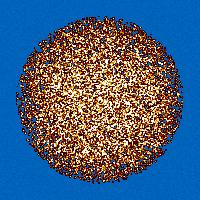
\includegraphics[width=0.95\linewidth]{figures/burn-20-bstep0}
  \caption{Fresh}
  \label{fig:bstep0}
\end{subfigure}%
%
\begin{subfigure}{0.4\textwidth}
  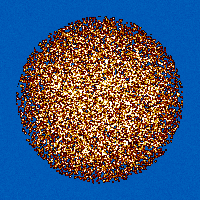
\includegraphics[width=0.95\linewidth]{figures/burn-20-bstep1}
  \caption{One Pass}
  \label{fig:bstep1}
\end{subfigure}%

\caption{Mesh Figures For Single Pebble Burnup}
\end{figure}

\begin{figure}[H]\ContinuedFloat
\centering

\begin{subfigure}{0.4\textwidth}
  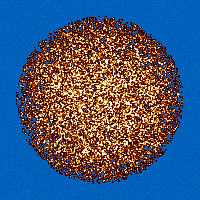
\includegraphics[width=0.95\linewidth]{figures/burn-20-bstep2}
  \caption{Two Passes}
  \label{fig:bstep2}
\end{subfigure}%
%
\begin{subfigure}{0.4\textwidth}
  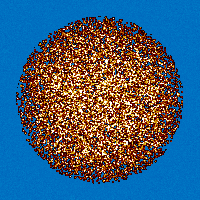
\includegraphics[width=0.95\linewidth]{figures/burn-20-bstep3}
  \caption{Three Passes}
  \label{fig:bstep3}
\end{subfigure}%

\begin{subfigure}{0.4\textwidth}
  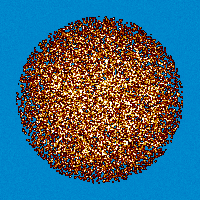
\includegraphics[width=0.95\linewidth]{figures/burn-20-bstep4}
  \caption{Four Passes}
  \label{fig:bstep4}
\end{subfigure}%
%
\begin{subfigure}{0.4\textwidth}
  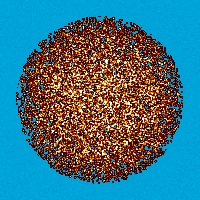
\includegraphics[width=0.95\linewidth]{figures/burn-20-bstep5}
  \caption{Five Passes}
  \label{fig:bstep5}
\end{subfigure}%

\begin{subfigure}{0.4\textwidth}
  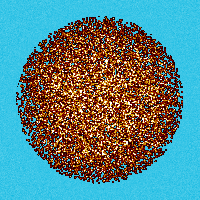
\includegraphics[width=0.95\linewidth]{figures/burn-20-bstep6}
  \caption{Six Passes}
  \label{fig:bstep6}
\end{subfigure}%
%
\caption{Mesh Figures For Single Pebble Burnup(cont.)}
\label{fig:burn-meshes}
\end{figure}
Figure \ref{fig:burn-meshes} provides the evolution of the fission rate (hot color map) and thermal flux (cold color map) over the 7 stages of burnup.  The maximum cutoff for thermal flux is 0.625 eV in these figures.  As one might expect, the fission rate decreases over subsequent depletion steps, and thermal flux decreases.
\begin{figure}[H]
\centering
%
\begin{subfigure}{0.8\textwidth}
  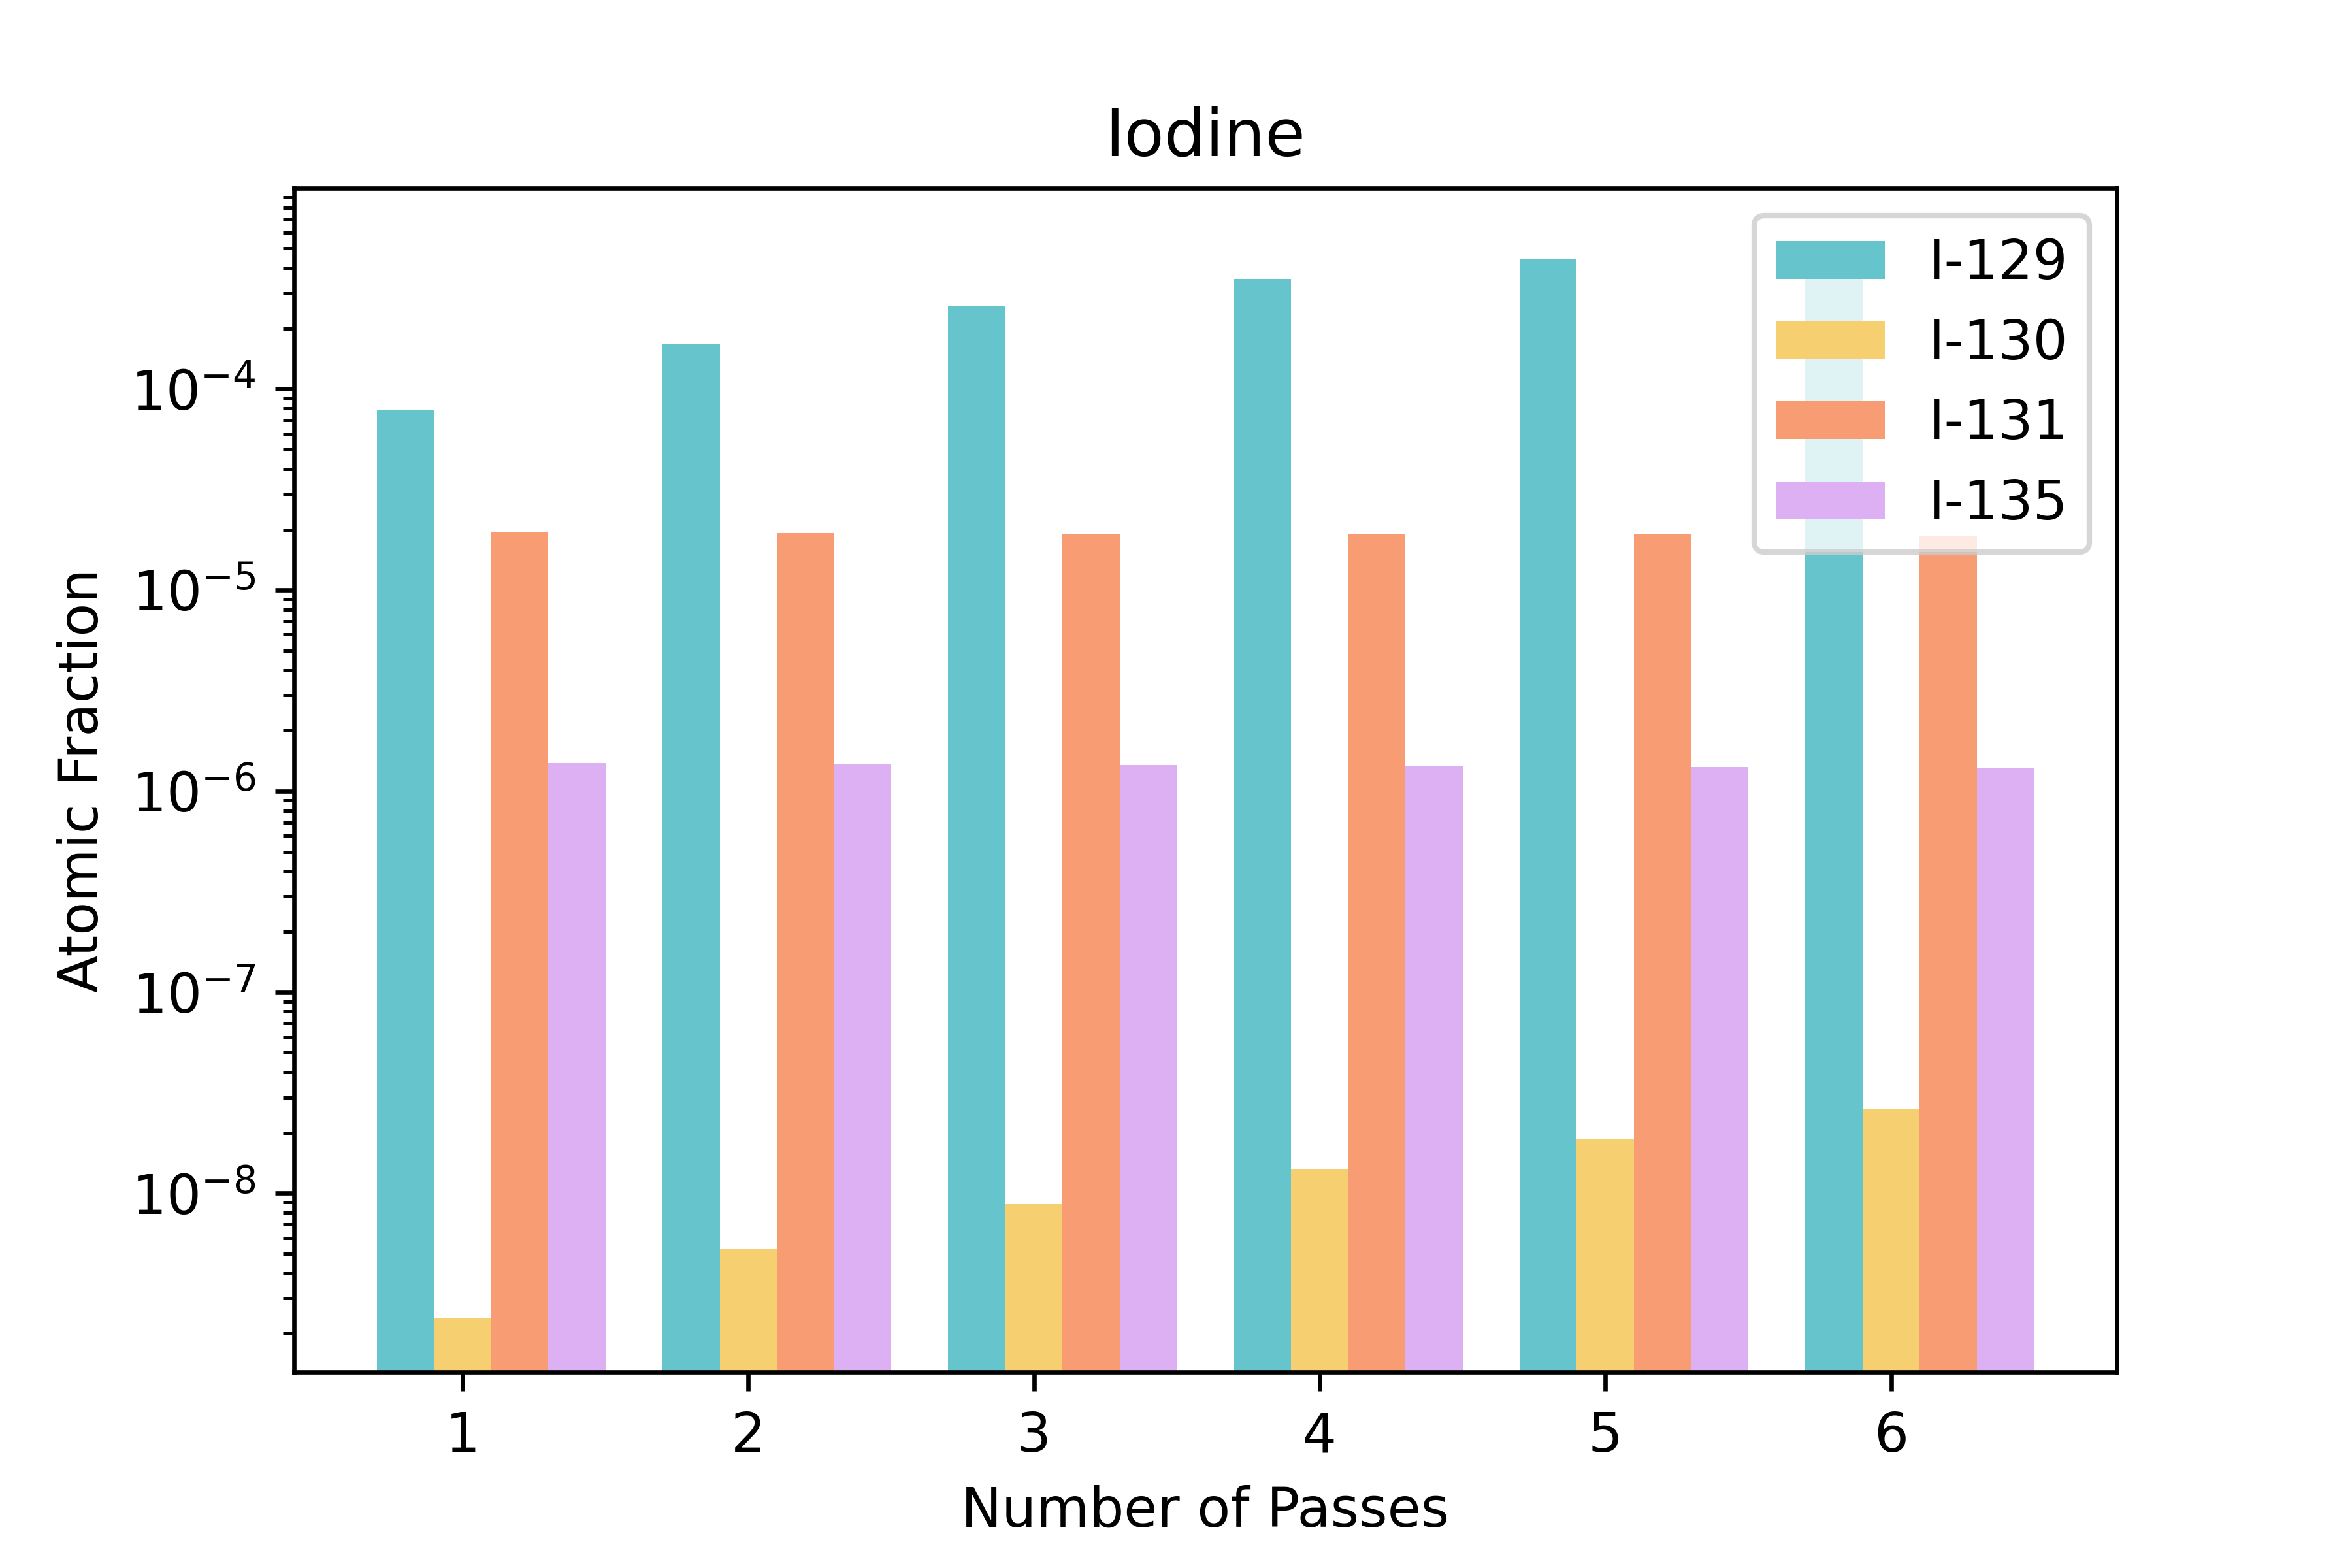
\includegraphics[width=\linewidth]{figures/compositions/iodine}
  \caption{Iodine isotope buildup over six burnup stages}
  \label{fig:i}
\end{subfigure}%

\begin{subfigure}{0.8\textwidth}
  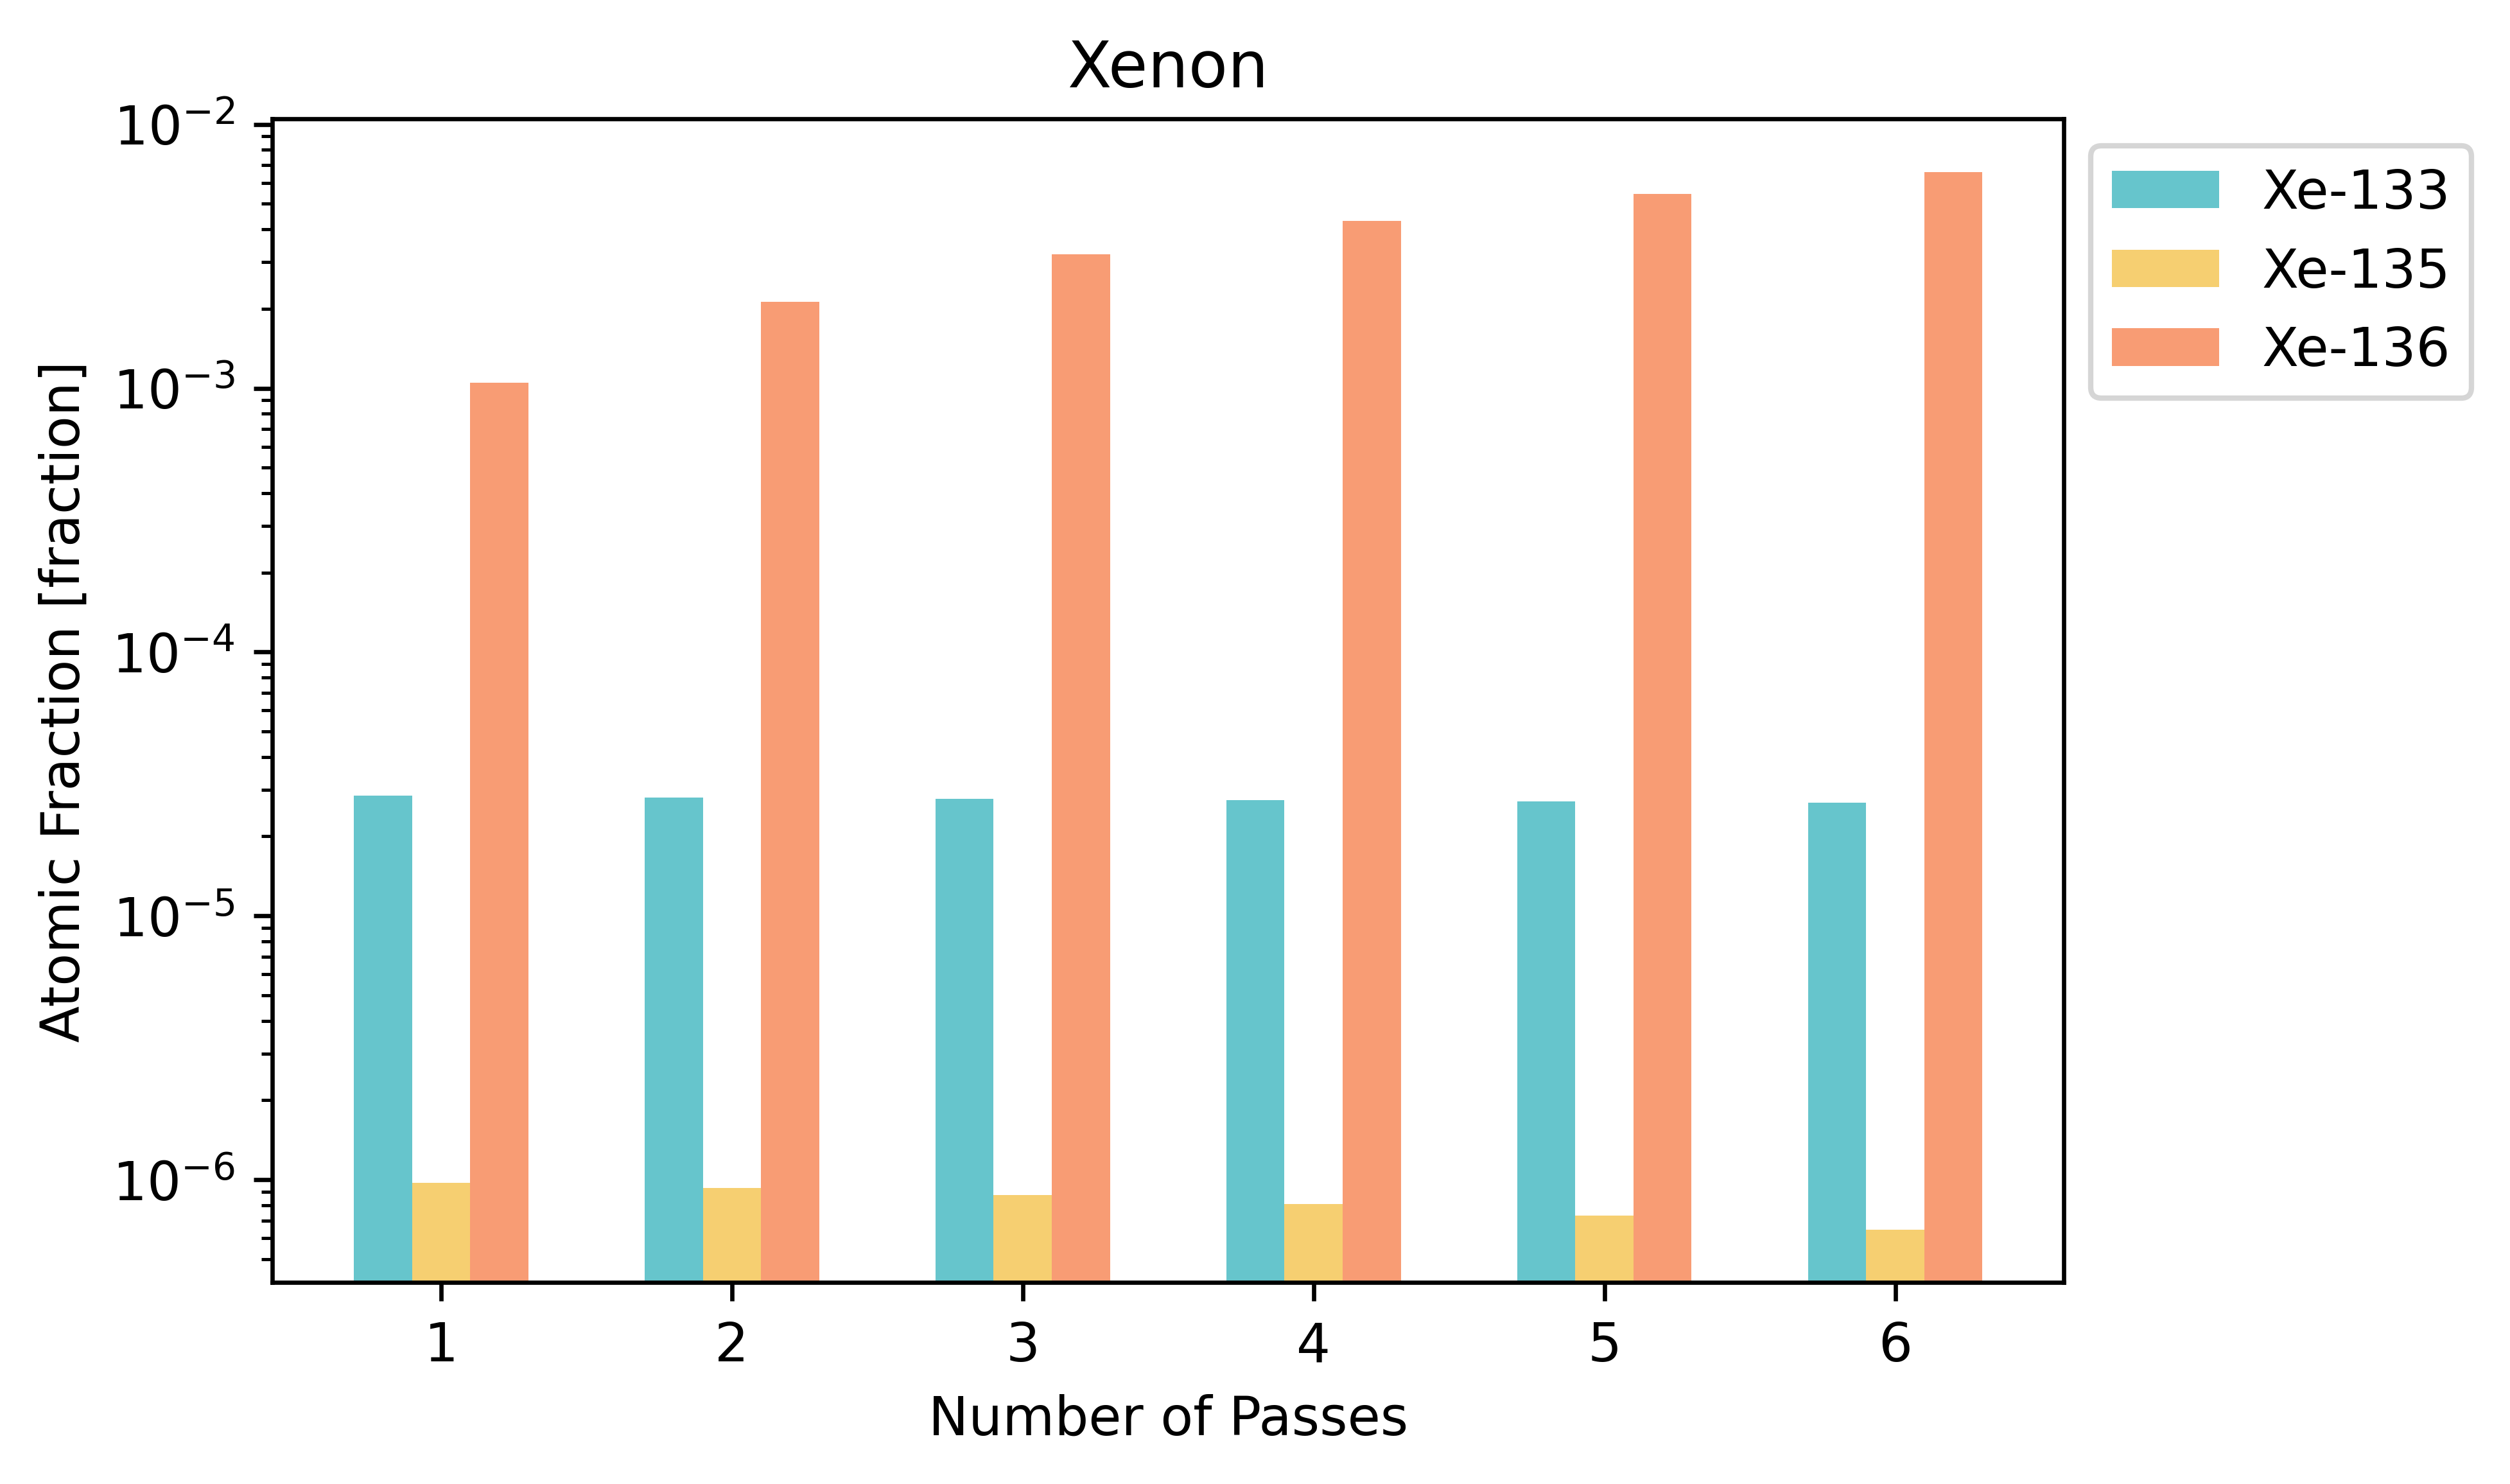
\includegraphics[width=\linewidth]{figures/compositions/xenon}
  \caption{Xenon isotope buildup over six burnup stages}
  \label{fig:xe}
\end{subfigure}%

\caption[Evolution of Safety Relevant Isotopic Concentrations in Pebbles of Sangamon20 over Six Six-Month Passes]{Evolution of Safety Relevant Isotopic Concentrations in Pebbles of Sangamon20 over Six Six-Month Passes (measured in atomic fraction)}
\end{figure}

\begin{figure}[H]\ContinuedFloat
\centering

\begin{subfigure}{0.8\textwidth}
  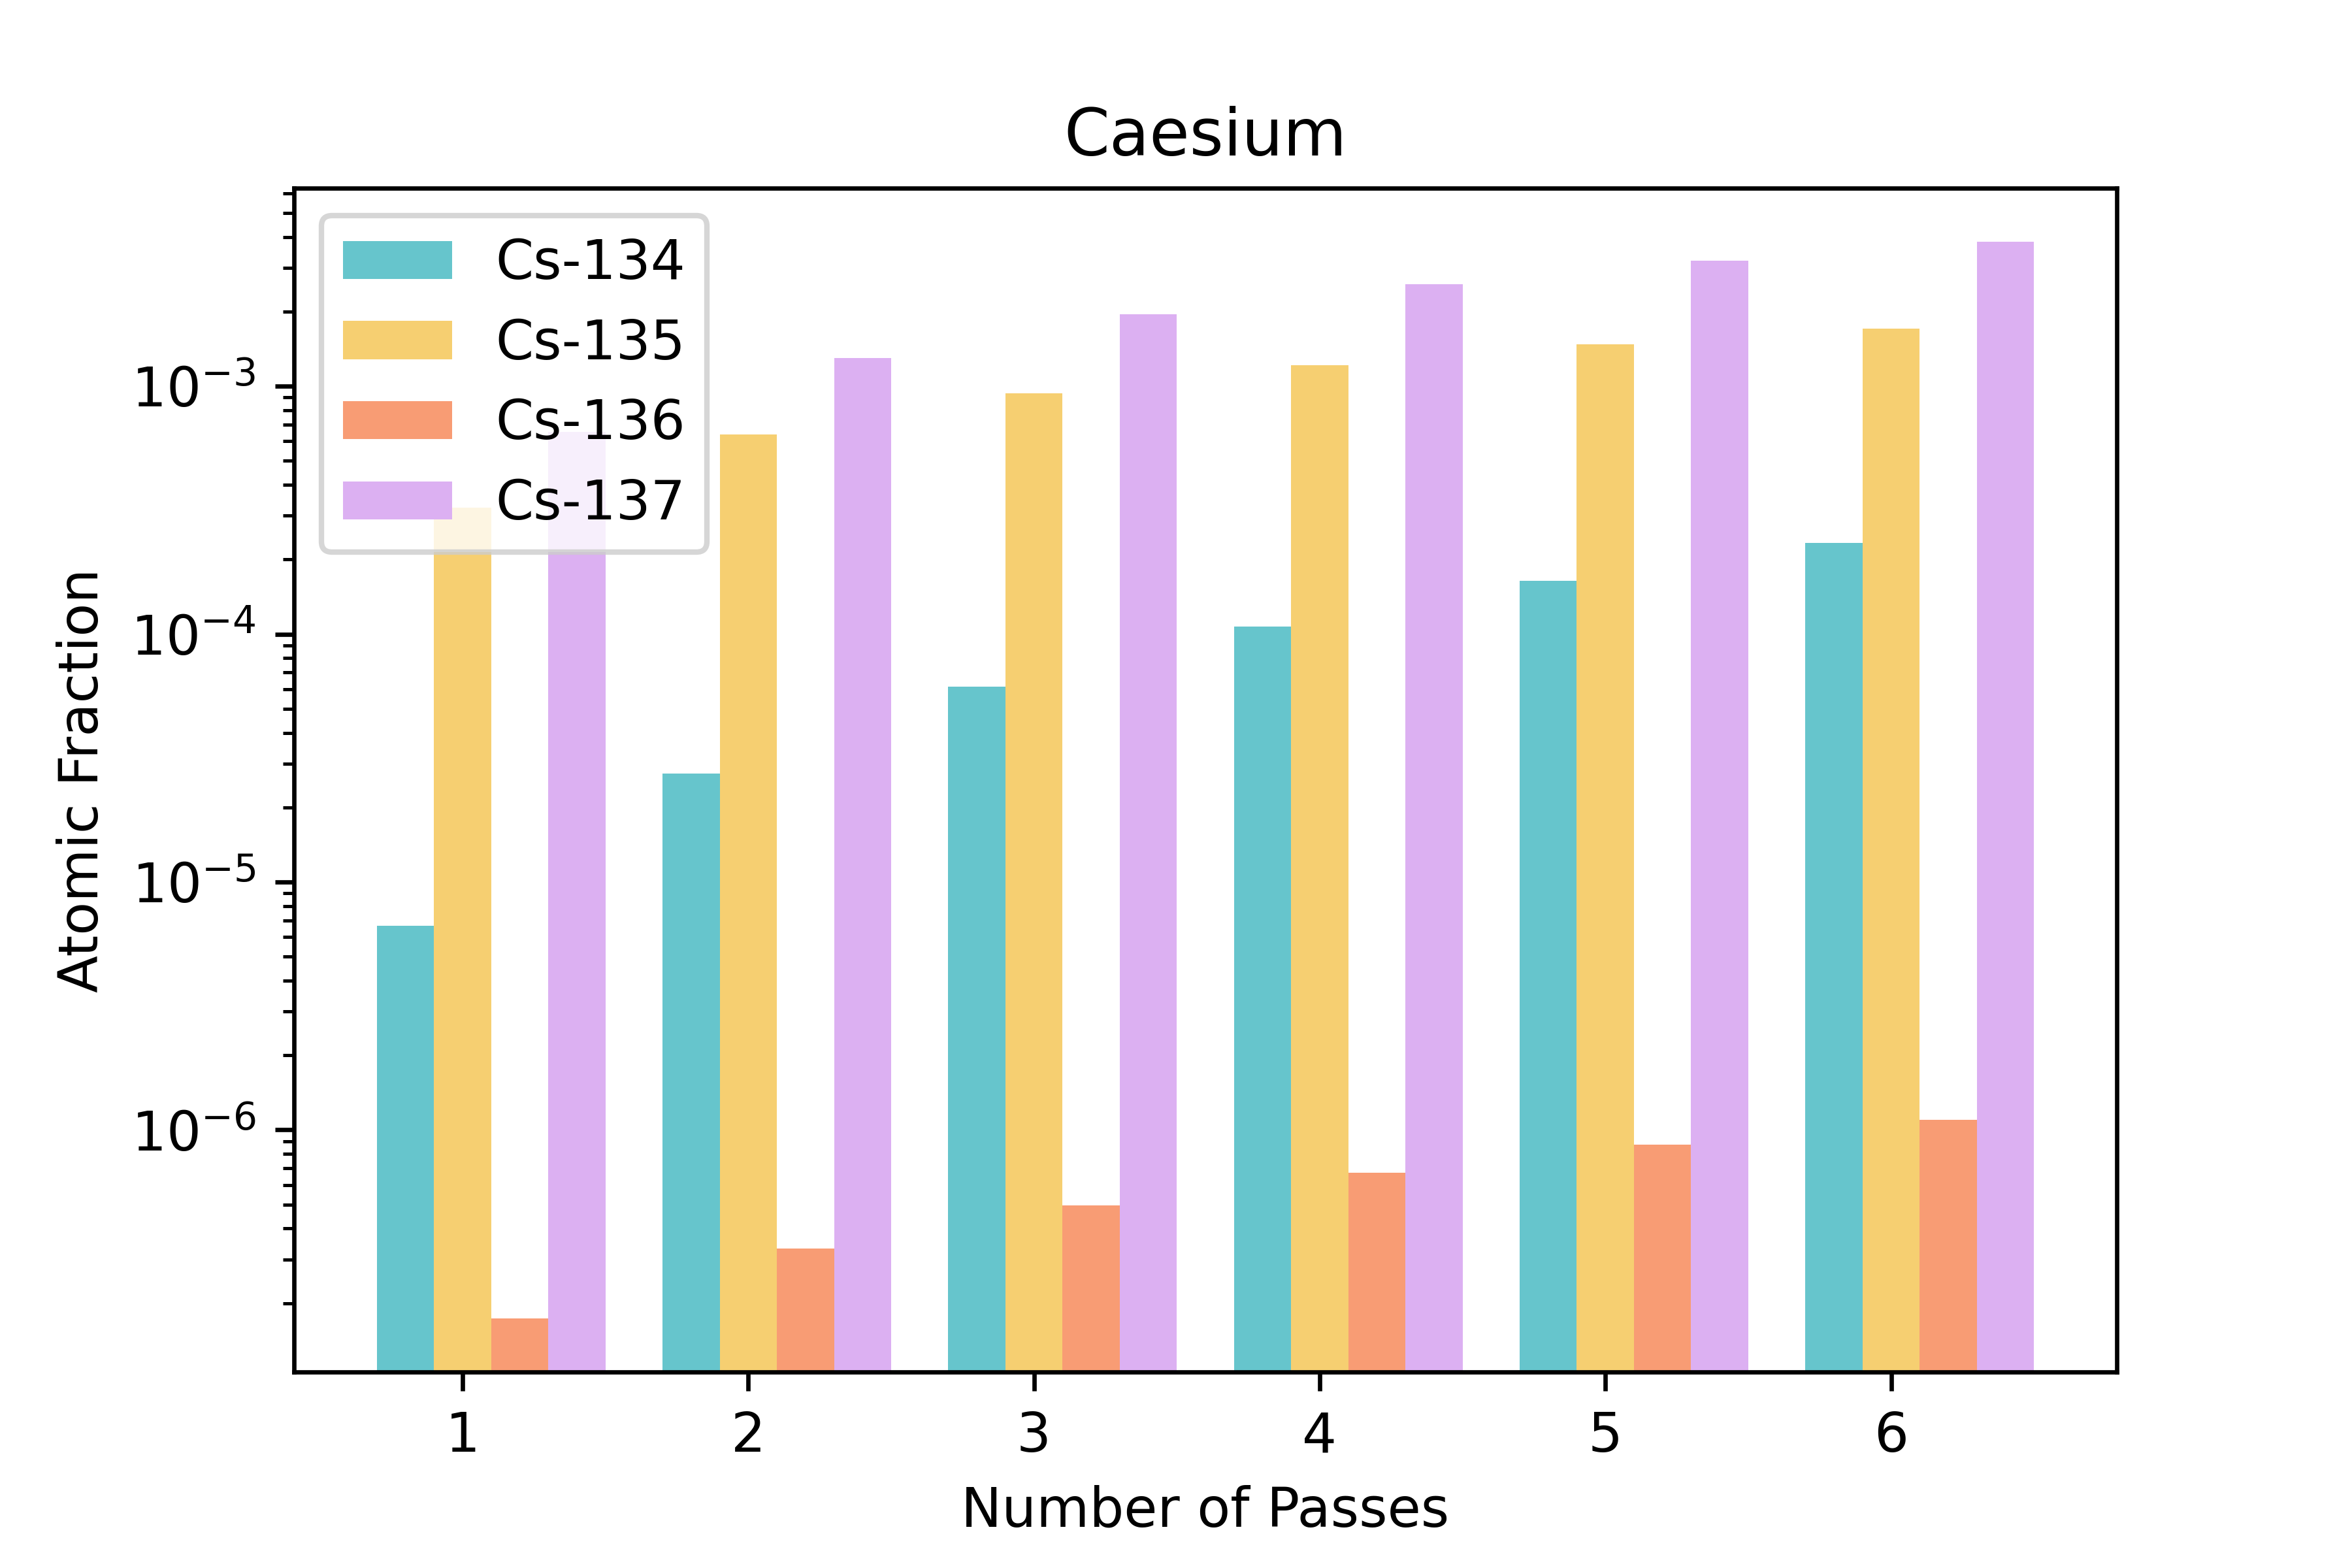
\includegraphics[width=\linewidth]{figures/compositions/caesium}
  \caption{Cesium isotope buildup over six burnup stages}
  \label{fig:cs}
\end{subfigure}%


\begin{subfigure}{0.8\textwidth}
  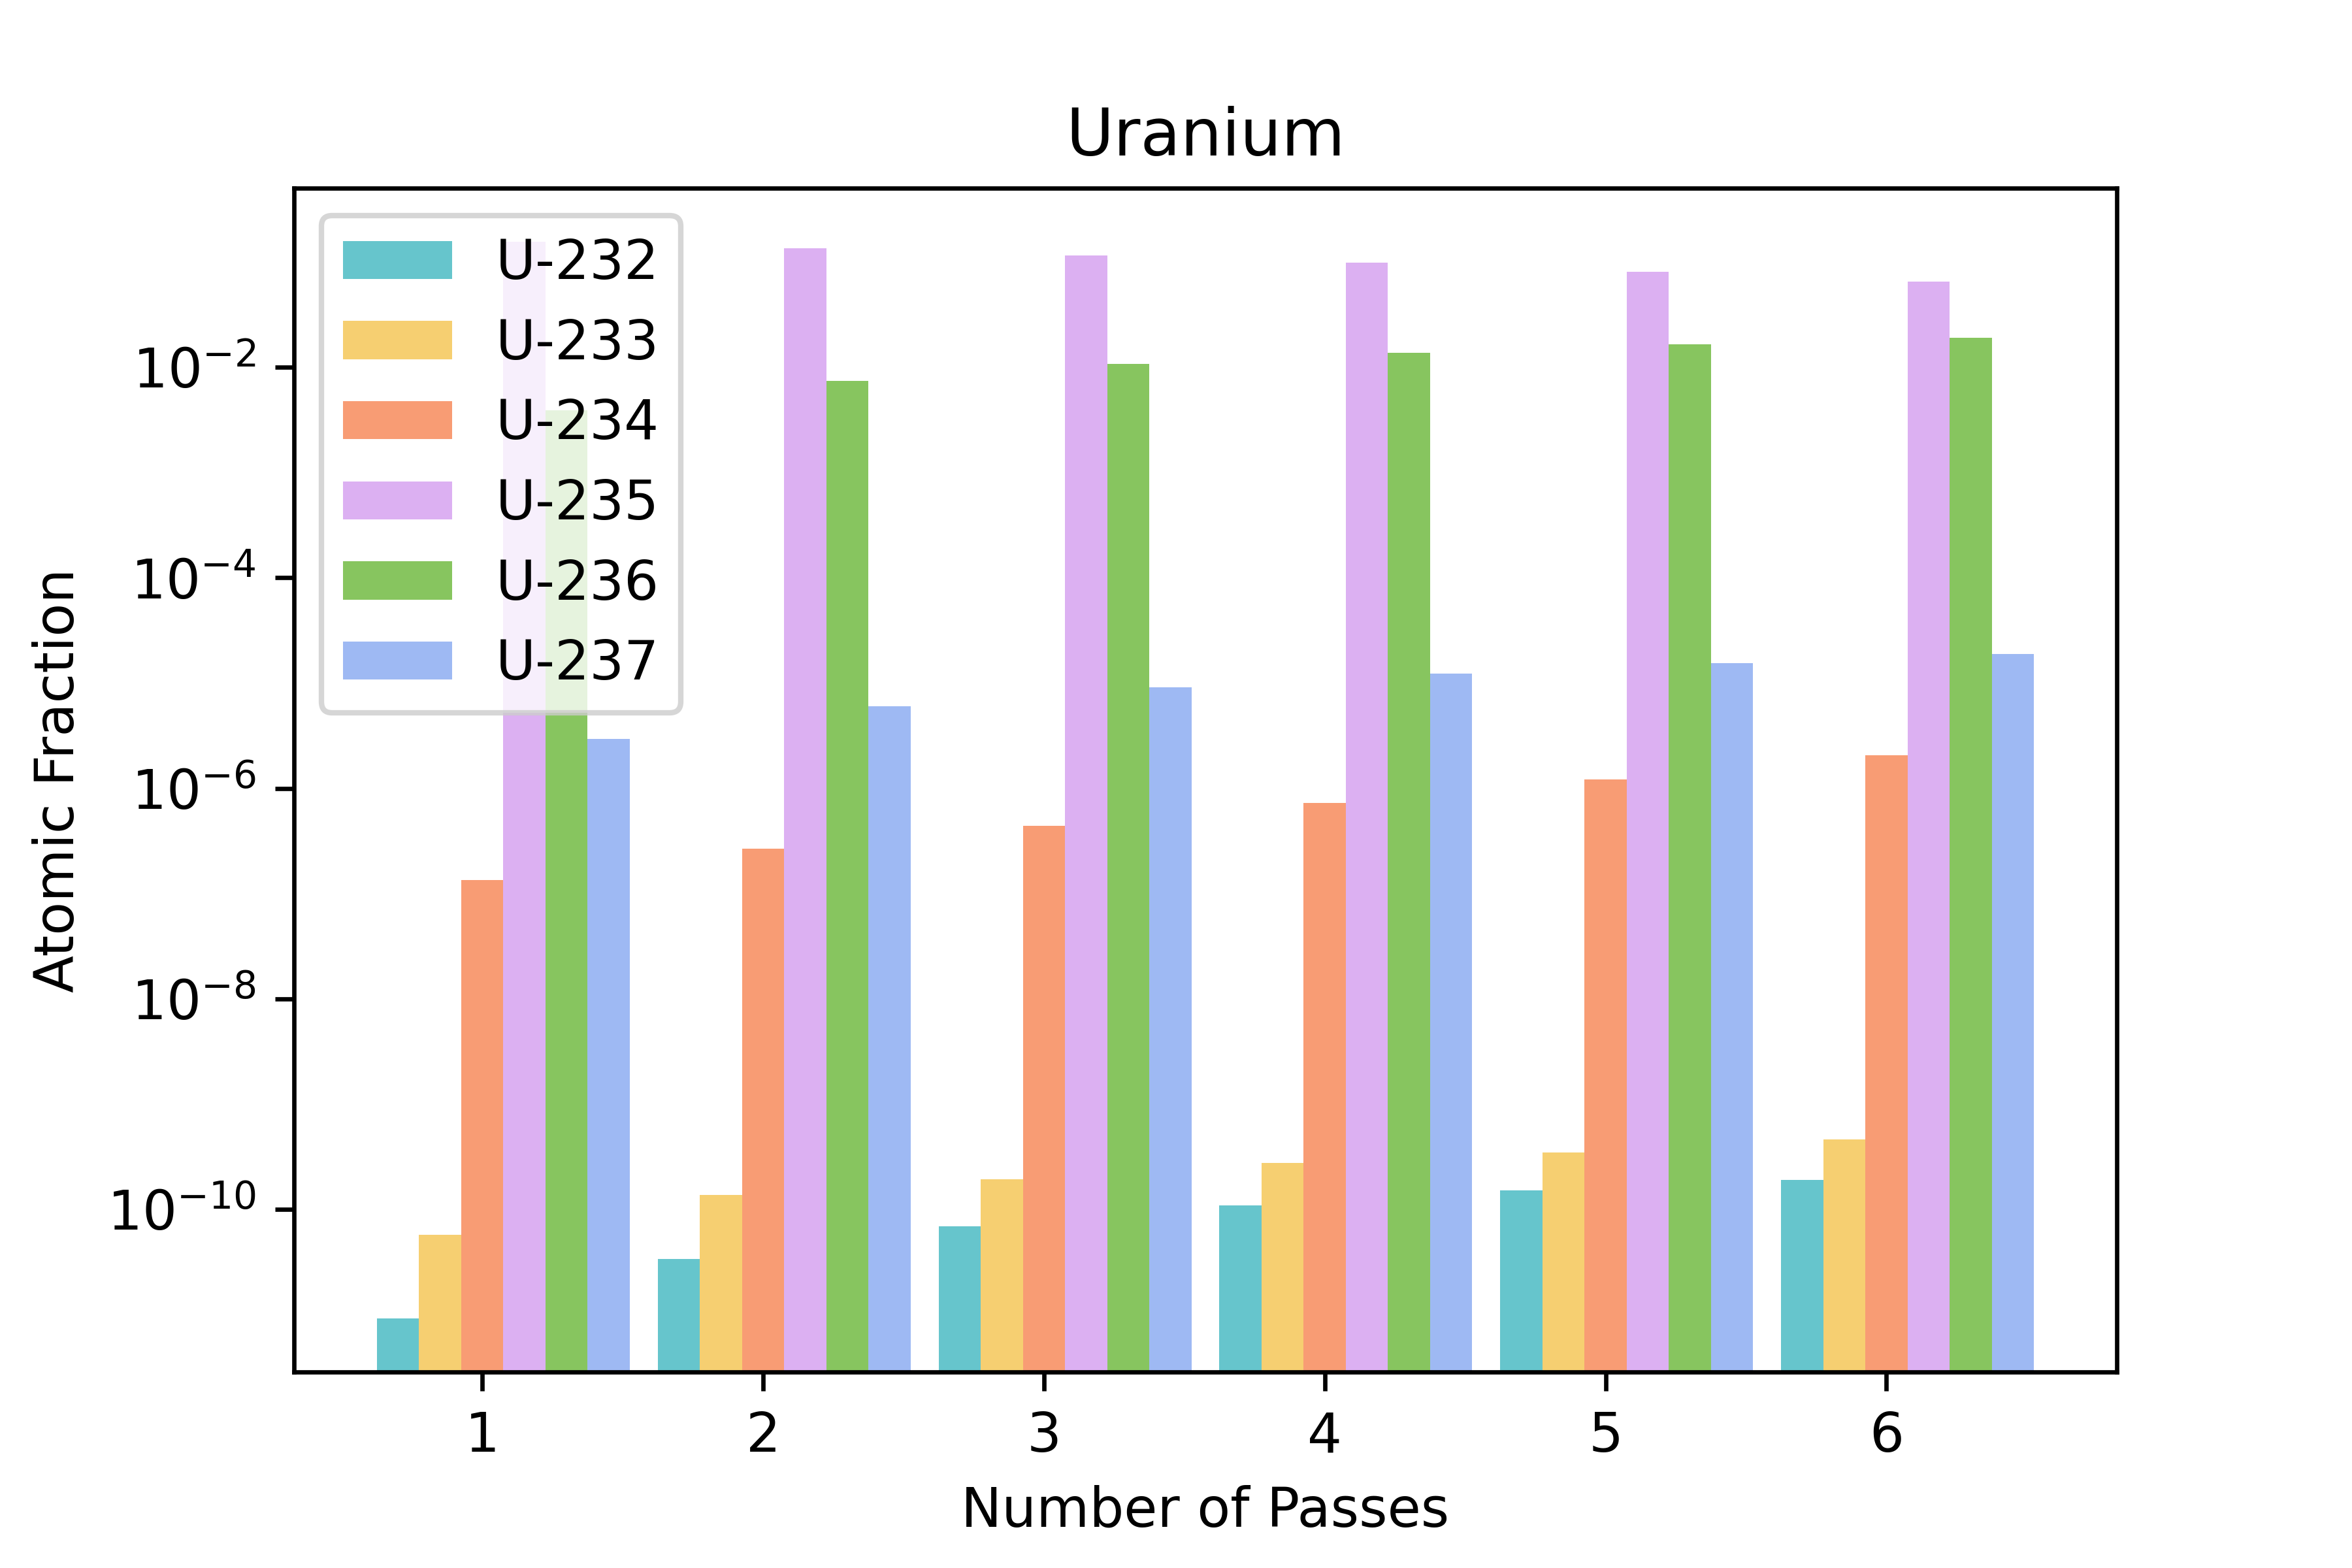
\includegraphics[width=\linewidth]{figures/compositions/uranium}
  \caption{Uranium isotope buildup over six burnup stages}
  \label{fig:u}
\end{subfigure}%

\caption[]{(cont.)}
\end{figure}

\begin{figure}[H]\ContinuedFloat
\centering

\begin{subfigure}{0.8\textwidth}
  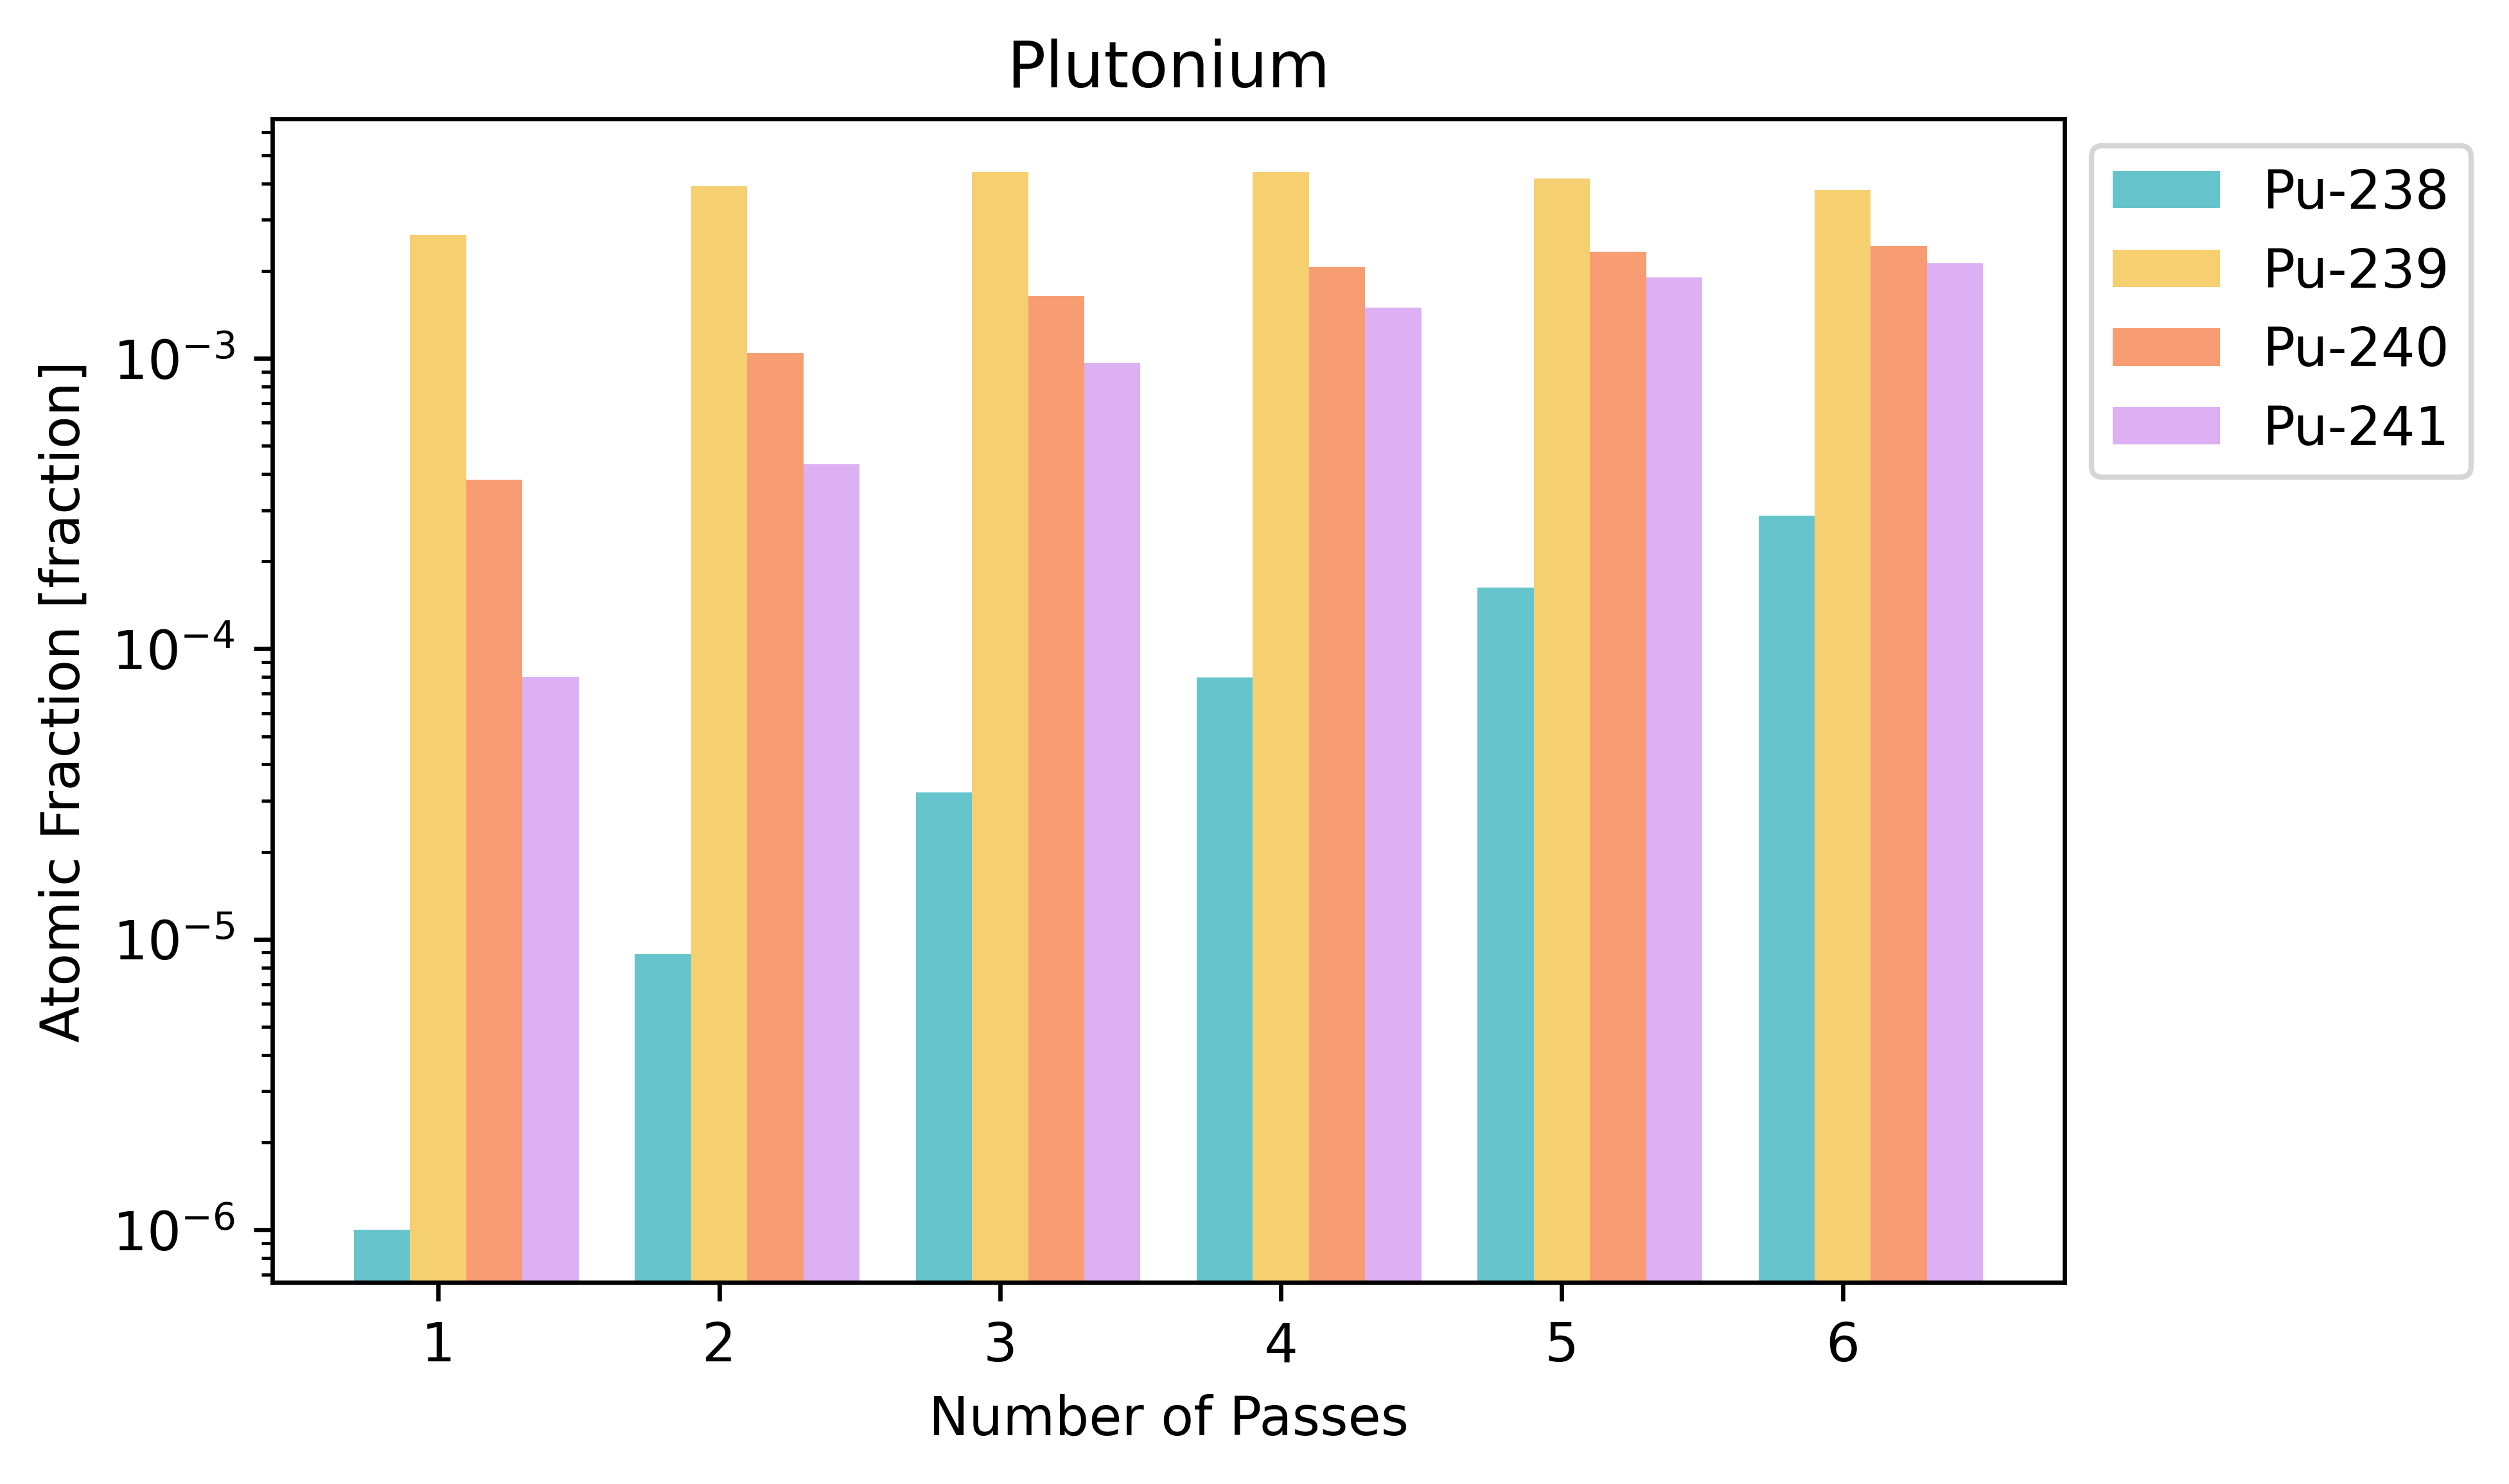
\includegraphics[width=\linewidth]{figures/compositions/plutonium}
  \caption{Plutonium isotope buildup over six burnup stages}
  \label{fig:pu}
\end{subfigure}%

\caption[]{(cont.)}
\label{fig:comps}
\end{figure}

***these definitely need to be resized, but I didn't want to take up too much space.  Should I try to fit 2 figures side by side, or should I do them one at a time?***

The full isotopic inventory tracked in the Sangamon20 reactor models extends far beyond those supplied in \ref{fig:comps}.  For a full list, see ***ref zenodo comps*** for the compositions alone, or ***ref phlox zenodo*** for a complete input file and associated output.  The isotopes selected for \ref{fig:comps} are chosen as they are commonly of interest in reactor physics or safety analysis, and any stable isotopes have been omitted from \ref{fig:comps}.

The inventory of uranium is, of course, quite large, rivaled only by the xenon content.  All isotopes of uranium steadily increase over time with the exception of U-235, which is lost as it undergoes fission, ending at 0.0647 by atomic fraction in the sixth pass.  U-232, while accounting for the smallest fraction of uranium content, also sees the most dramatic increase over time, increasing by two orders of magnitude between its first (9.28E-12) and sixth (1.9E-10) cycle.  While the atomic fraction doesn't reach an equilibrium, the rate at which it increase each cycle is steady by the third pass, increasing by 4.02E-11,4.2E-11, and 3.9E-11 from the third to fourth, fourth to fifth, and fifth to sixth pass, respectively.  Plutonium content is also fairly high, with Pu-239 peaking at 0.00439.  However, unlike many other isotopes which peak in the sixth cycle, Pu-239 crests in the third and fourth passes, only to decrease from 0.00439 in the fourth pass to 0.00380 in the sixth.  Pu-238, meanwhile is the least abundant, but does experience the most dramatic increase over time, especially between the first and second passes.



Xe-133 seems to be steady around its initial value of 2.86E-05 atomic fraction, decreasing only to 2.68E-05 by the sixth pass.  Xe-135 decreases a bit more dramatically, going from an inital 9.7E-07 after its first six months, to  6.46E-07 after thirty-six months.  Xe-136 is both the greatest contributor to xenon content in the fuel, and the only isotope reported in \ref{fig:xe} to increase, owing to its long half life.  Each cycle, Xe-136 content increases by ~0.0011, beginning at a concentration of 0.00105 in the first cycle and ending at 0.0066 after the sixth.  Isotopes of iodine form a smaller portion of FPs than xenon or caesium, but is still of a relatively high magnitude, and is of concern due to its high mobility in water and uptake in the thyroid.  I-129 is the most abundant isotope of iodine reported here, and increases for the entirety of the pebble's life, beginning at 7.38E-05 and peaking at 0.000538 at its discharge burnup.  I-130 and I-135 are both relatively stable, most likely due to their short half-lives.  I-130 is the least abundant, but increases over time.  Caesium has a concentration similar to xenon's, if a bit smaller.  Unsurprisingly, Cs-135 and Cs-137, which both have half-lives longer than a pebble's stint in the reactor, are in greatest abundance, and increase over time.

Of the elements reported here, radium and thorium are in lowest abundance.  Ra-225 only appears in trace amounts (less than or equal to 9.99E-20) for the first three passes.  Ra-224 far outweighs the other reported isotopes of radium, with an atomic fraction of 7.46E-15 after thirty-six months - two orders of magnitude higher than all other isotopes of radium combined at this depletion step.  Thorium has the second-least abundant atomic fractions, with fertile Th-232 being the most abundant, at 8.8E-10 in the sixth pass.

\section{Full-Core Control Model}

Figure \ref{fig:control} shows a cross section of the core geometry at the origin in the xy and xz planes (a and c, respectively) and provides a mesh of the fission rate and thermal flux in the xy and xz planes (b and d, respectively).  Both of these are integrated to produce a 2D image.
\begin{figure}[h!]
\centering
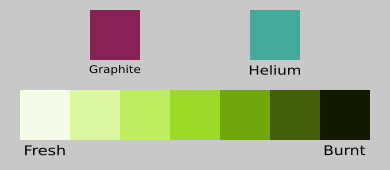
\includegraphics[width=0.6\linewidth]{figures/geom-legend}
\caption{Legend for Geometry Figures}
\label{fig:geom-legend}
\end{figure}

Figure \ref{fig:geom-legend} is accurate for all cross sections of reactor geometry.  In homogenized models, the shades of green represent the material blend forming the center of the pebble, at a given burnup.  For heterogenized models, these same shades represent the TRISO particle kernel at a particular burnup.

\begin{figure}[H]
\centering

\begin{subfigure}{0.45\textwidth}
  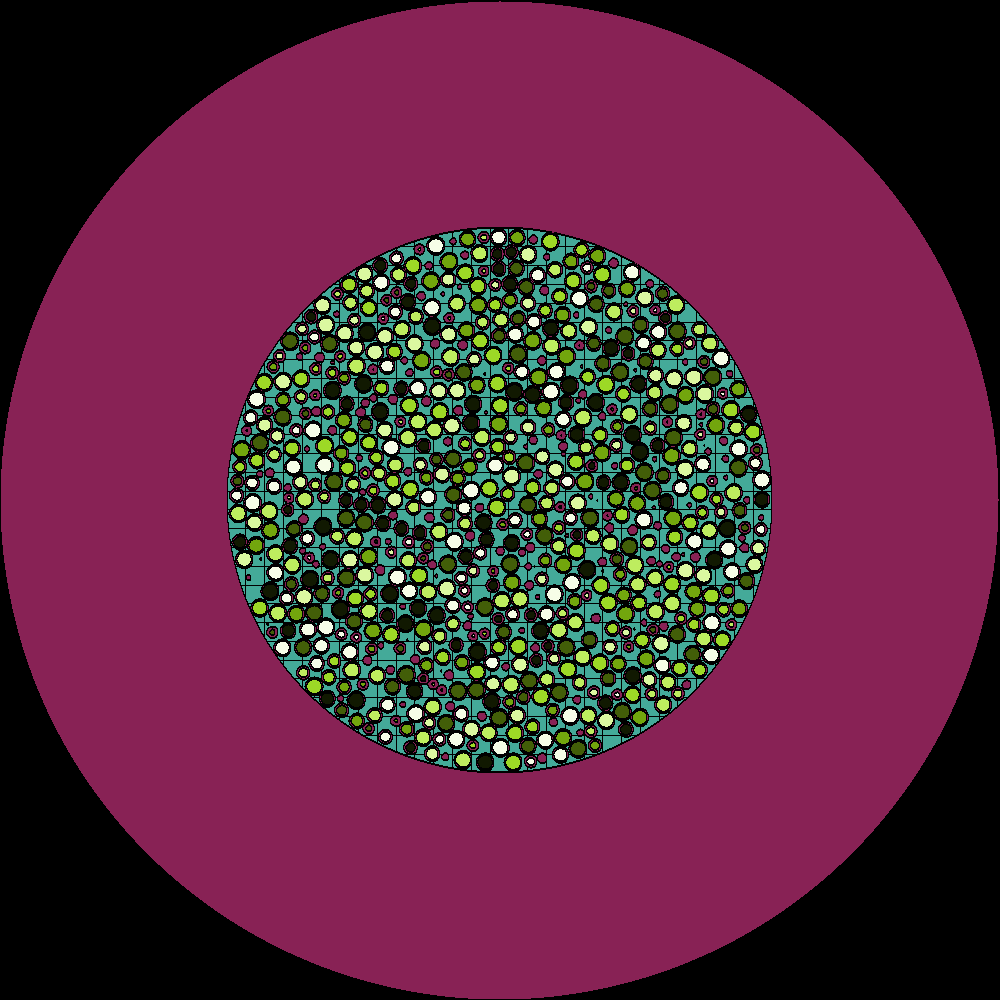
\includegraphics[width=0.95\linewidth]{figures/control/control-r}
  \caption{Radial Cross Section at y=0}
  \label{fig:controla}
\end{subfigure}%
%
\begin{subfigure}{0.45\textwidth}
  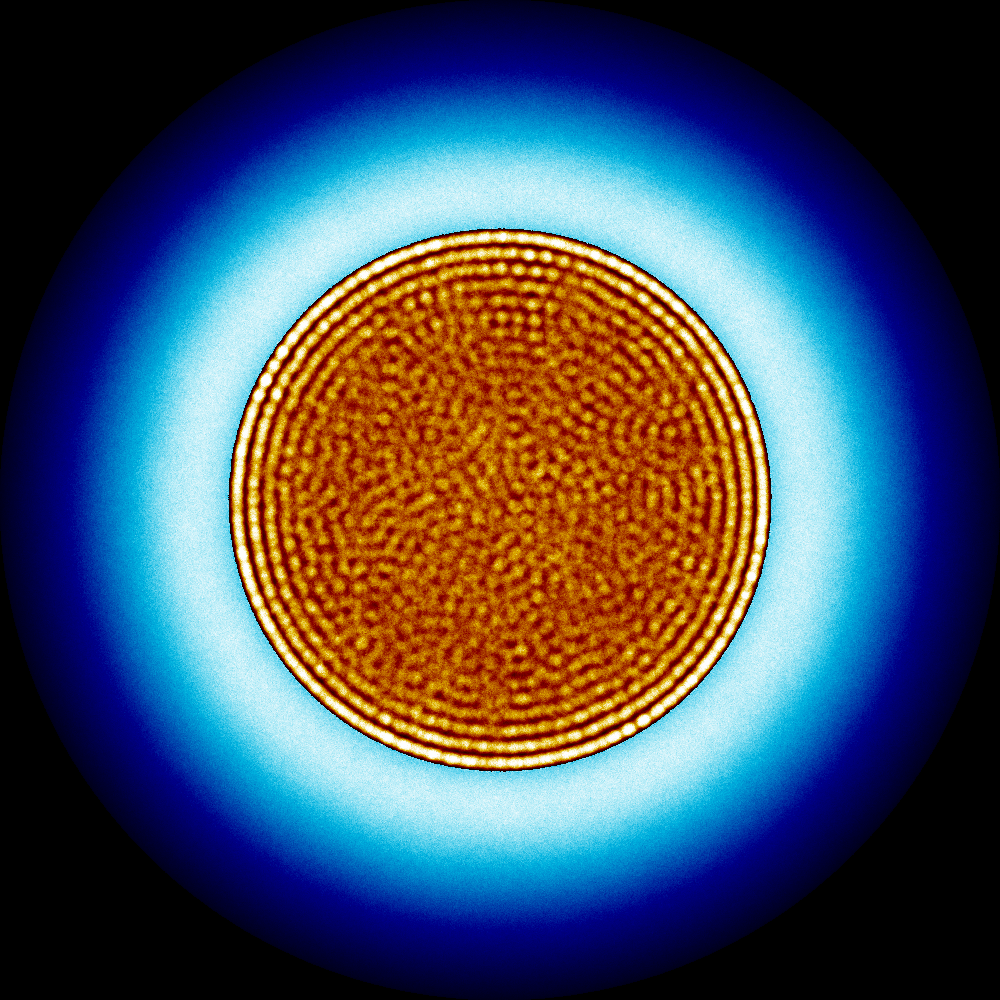
\includegraphics[width=0.95\linewidth]{figures/control/control-rm}
  \caption{Radial Mesh}
  \label{fig:controlb}
\end{subfigure}

\begin{subfigure}{0.45\textwidth}
  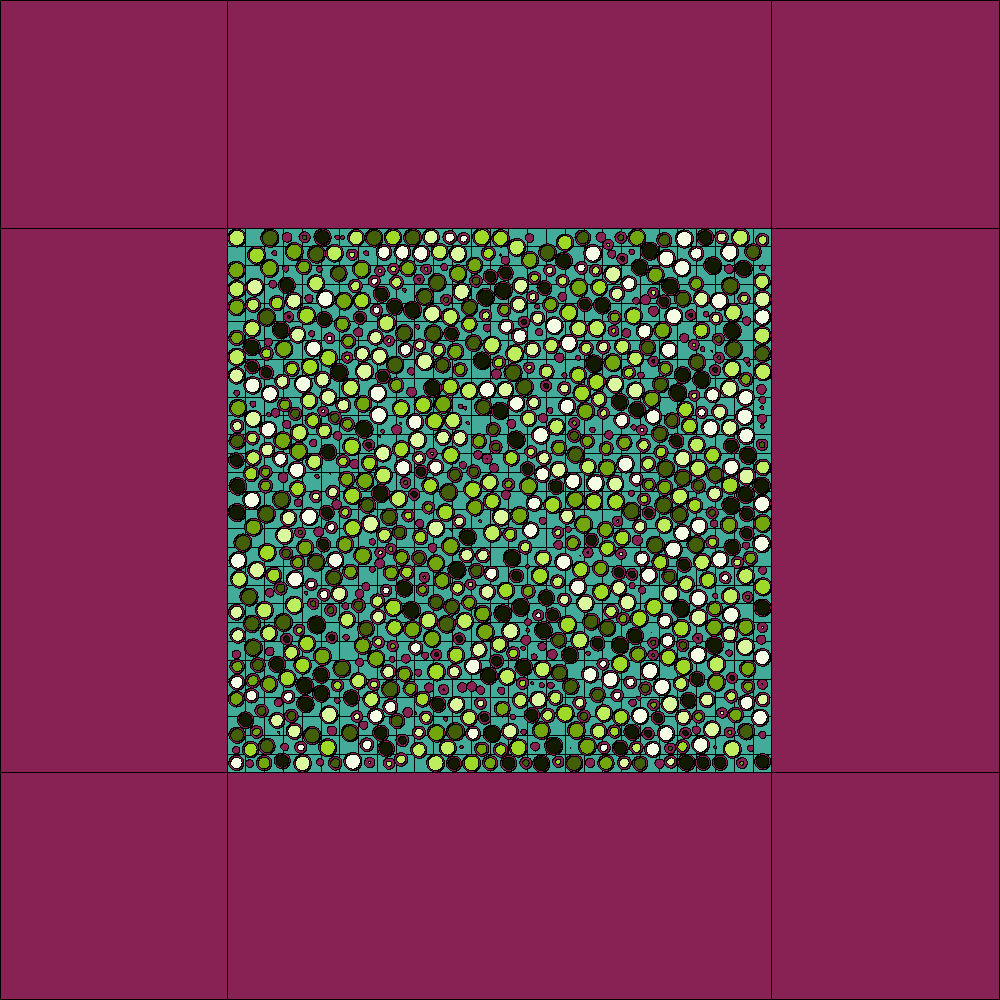
\includegraphics[width=0.95\linewidth]{figures/control/control-v}
  \caption{Axial Cross Section at z=0 }
  \label{fig:controlc}
\end{subfigure}
%
\begin{subfigure}{0.45\textwidth}
  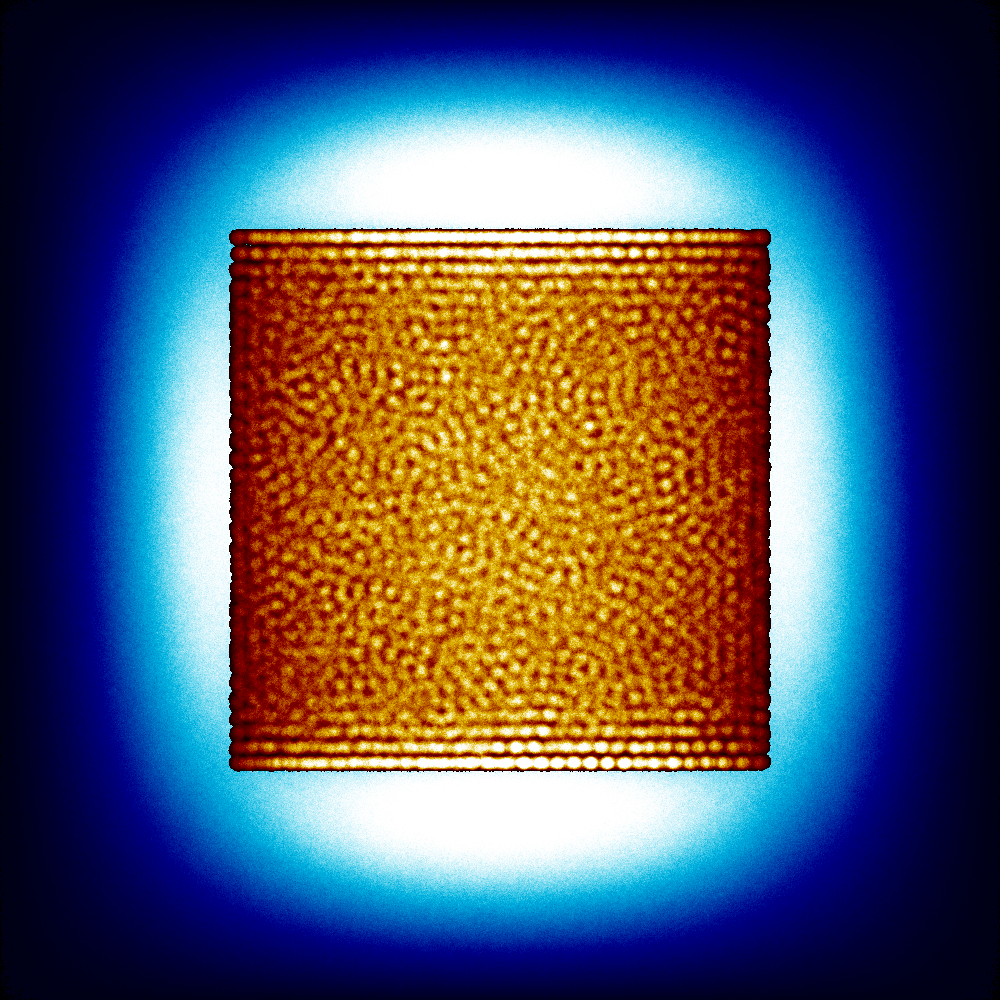
\includegraphics[width=0.95\linewidth]{figures/control/control-vm}
  \caption{Axial Mesh}
  \label{fig:controld}
\end{subfigure}
%
\begin{subfigure}{\textwidth}
\centering
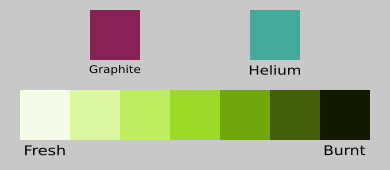
\includegraphics[width=0.6\linewidth]{figures/geom-legend}
\caption{Legend for \ref{fig:controla} and \ref{fig:controlc}}
\label{fig:geom-legend1}
\end{subfigure}

\caption{Geometry Cross Sections (left) and Thermal Flux(cold color map) and Fission Rate (hot color map) Meshes (right) for the Control Model of Sangamon20}
\label{fig:controlmain}
\end{figure}


The mesh in  \ref{fig:controlb} shows bands of concentric rings around the outer edges of the active core.  These bands would suggest that the outermost regions of the core are regions of high fission activity, relative to the center, which is at odds with what most would expect from the neutronics behavior in a cylindrical reactor.  Certainly, the pebbles are physically forming rings at the outer edges, and their placement becomes more haphazard toward the center.  However, the author asserts that the high intensities seen in this outer region in the mesh figures are not indicative of a total flux profile showing the same.  Remember that this image is generated by integrating over the z direction to produce a 2D plot of the xy plane.  For a cylinder, the distance in z each point integrates over is the same - the height of the reactor.  However, points at the outermost regions are integrating in a volume that is composed more of pebbles - and therefore fissile material - than the center, where there is more space filled with coolant.

In figure \ref{fig:controld}  we can see a similar banding effect on the top and bottom edge of the core region, but not on the sides.  There are no hotspots on the edges because \ref{fig:controld} is in the xz plane, and integrates over y.  However, for a cylinder, the distance integrated over is not the same at all points.  At the centerline, the distance is simply the diameter.  However, as you move towards the edge, the distance integrated over approaches zero.

\begin{figure}[H]
\centering

\begin{subfigure}{0.9\textwidth}
  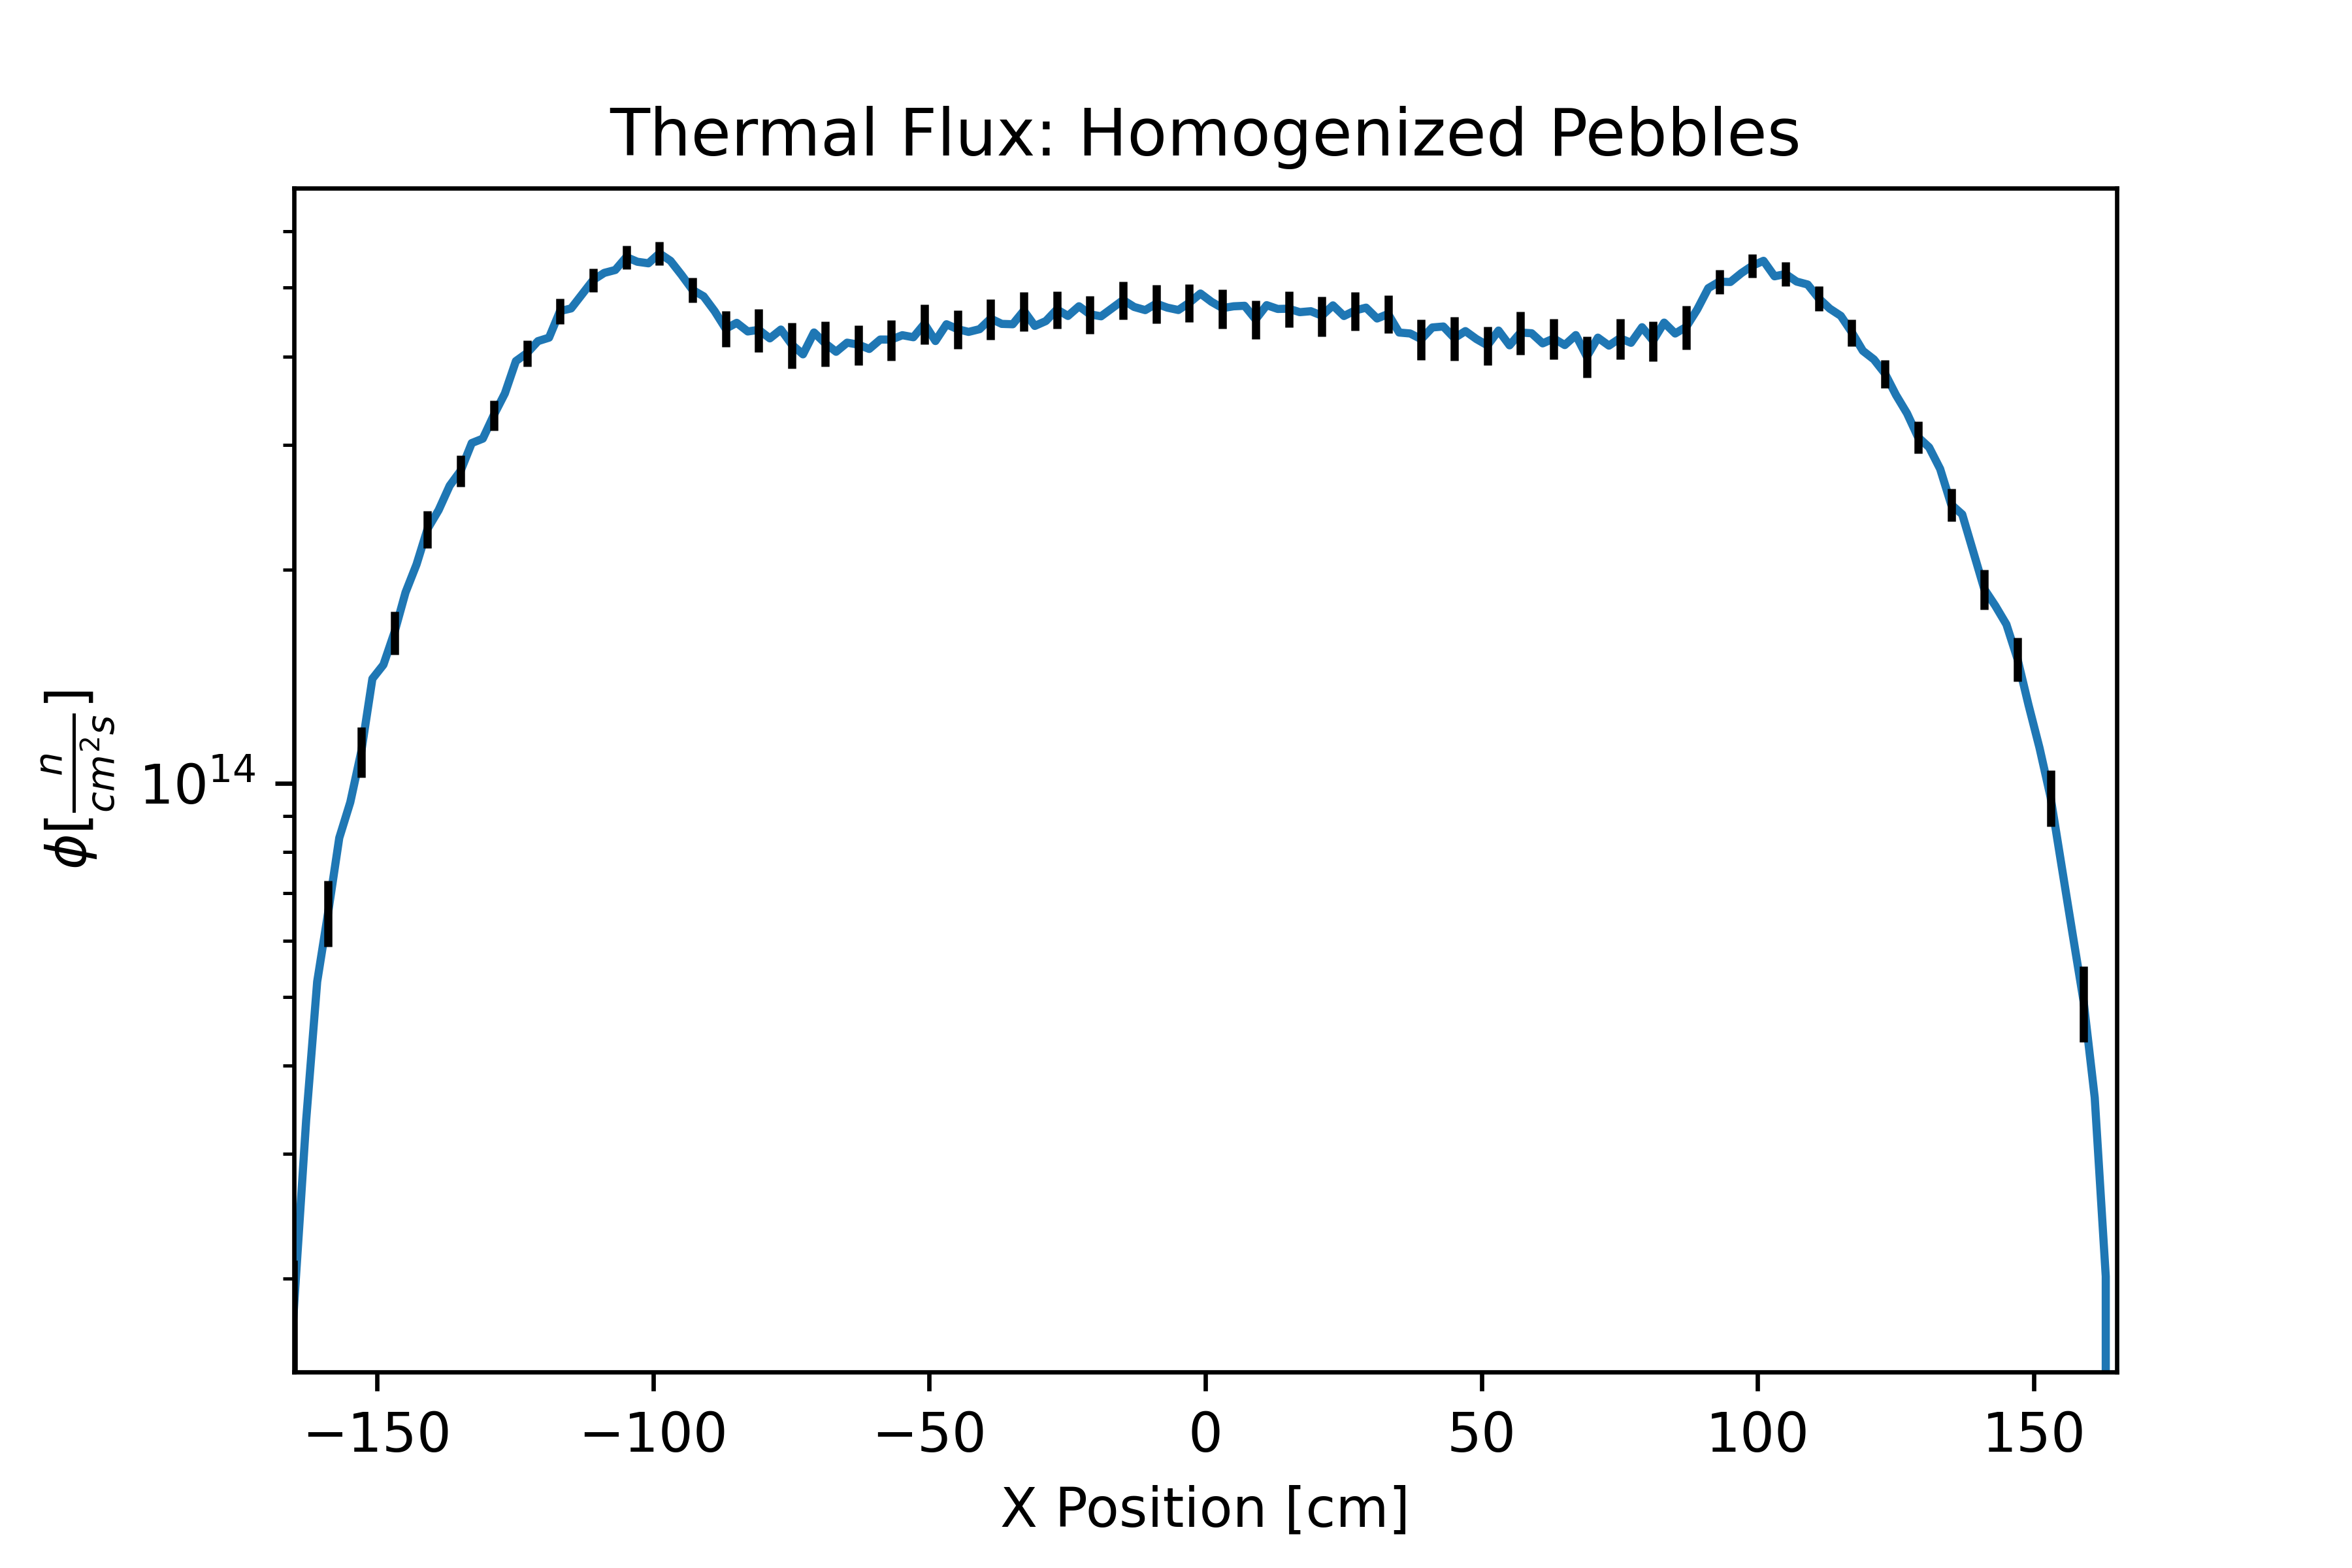
\includegraphics[width=0.95\linewidth]{figures/therm_flux_homog.png}
  \caption{Thermal Flux}
  \label{fig:hom-det-xy-therm}
\end{subfigure}%

\caption{Radial Thermal and Fast Flux Profiles}
\end{figure}

\begin{figure}[H]\ContinuedFloat
\centering

\begin{subfigure}{0.9\textwidth}
  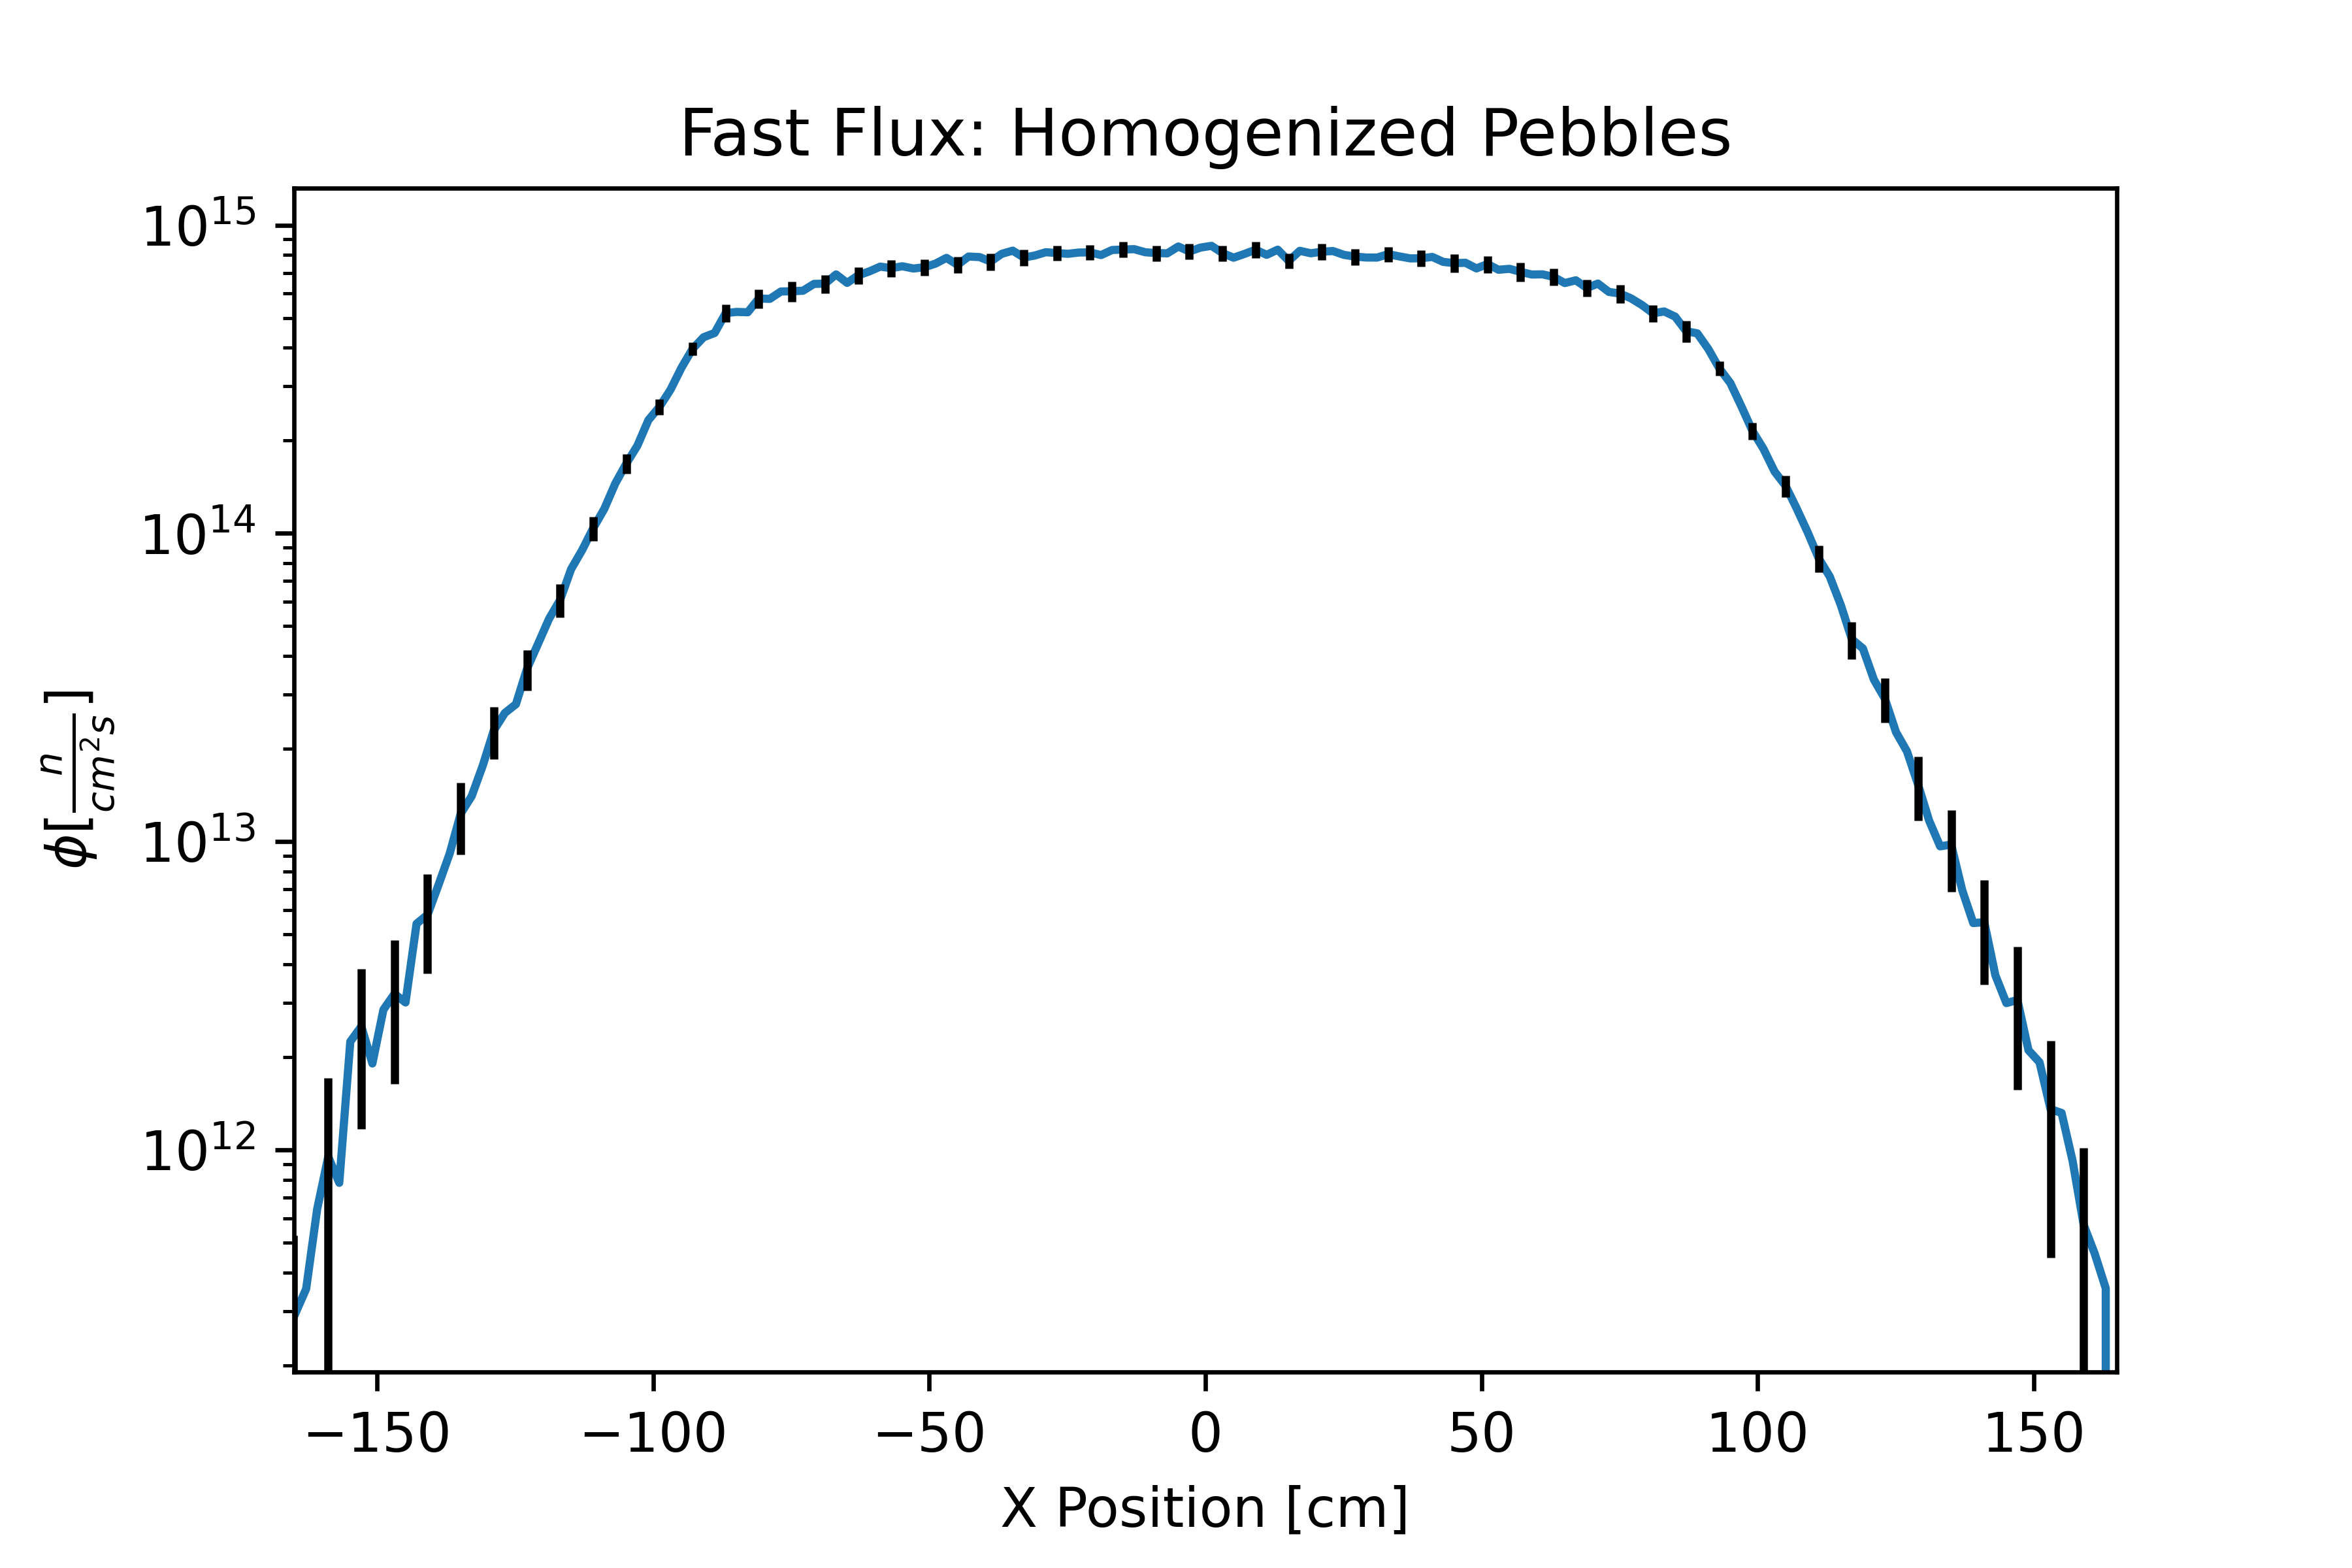
\includegraphics[width=0.95\linewidth]{figures/fast_flux_homog.png}
  \caption{Fast Flux}
  \label{fig:hom-det-xy-fast}
\end{subfigure}

%
\caption{Radial Thermal and Fast Flux Profiles (cont.)}
\label{fig:hom-det-xy}
\end{figure}
\begin{figure}[h!]
\centering

\begin{subfigure}{0.6\textwidth}
  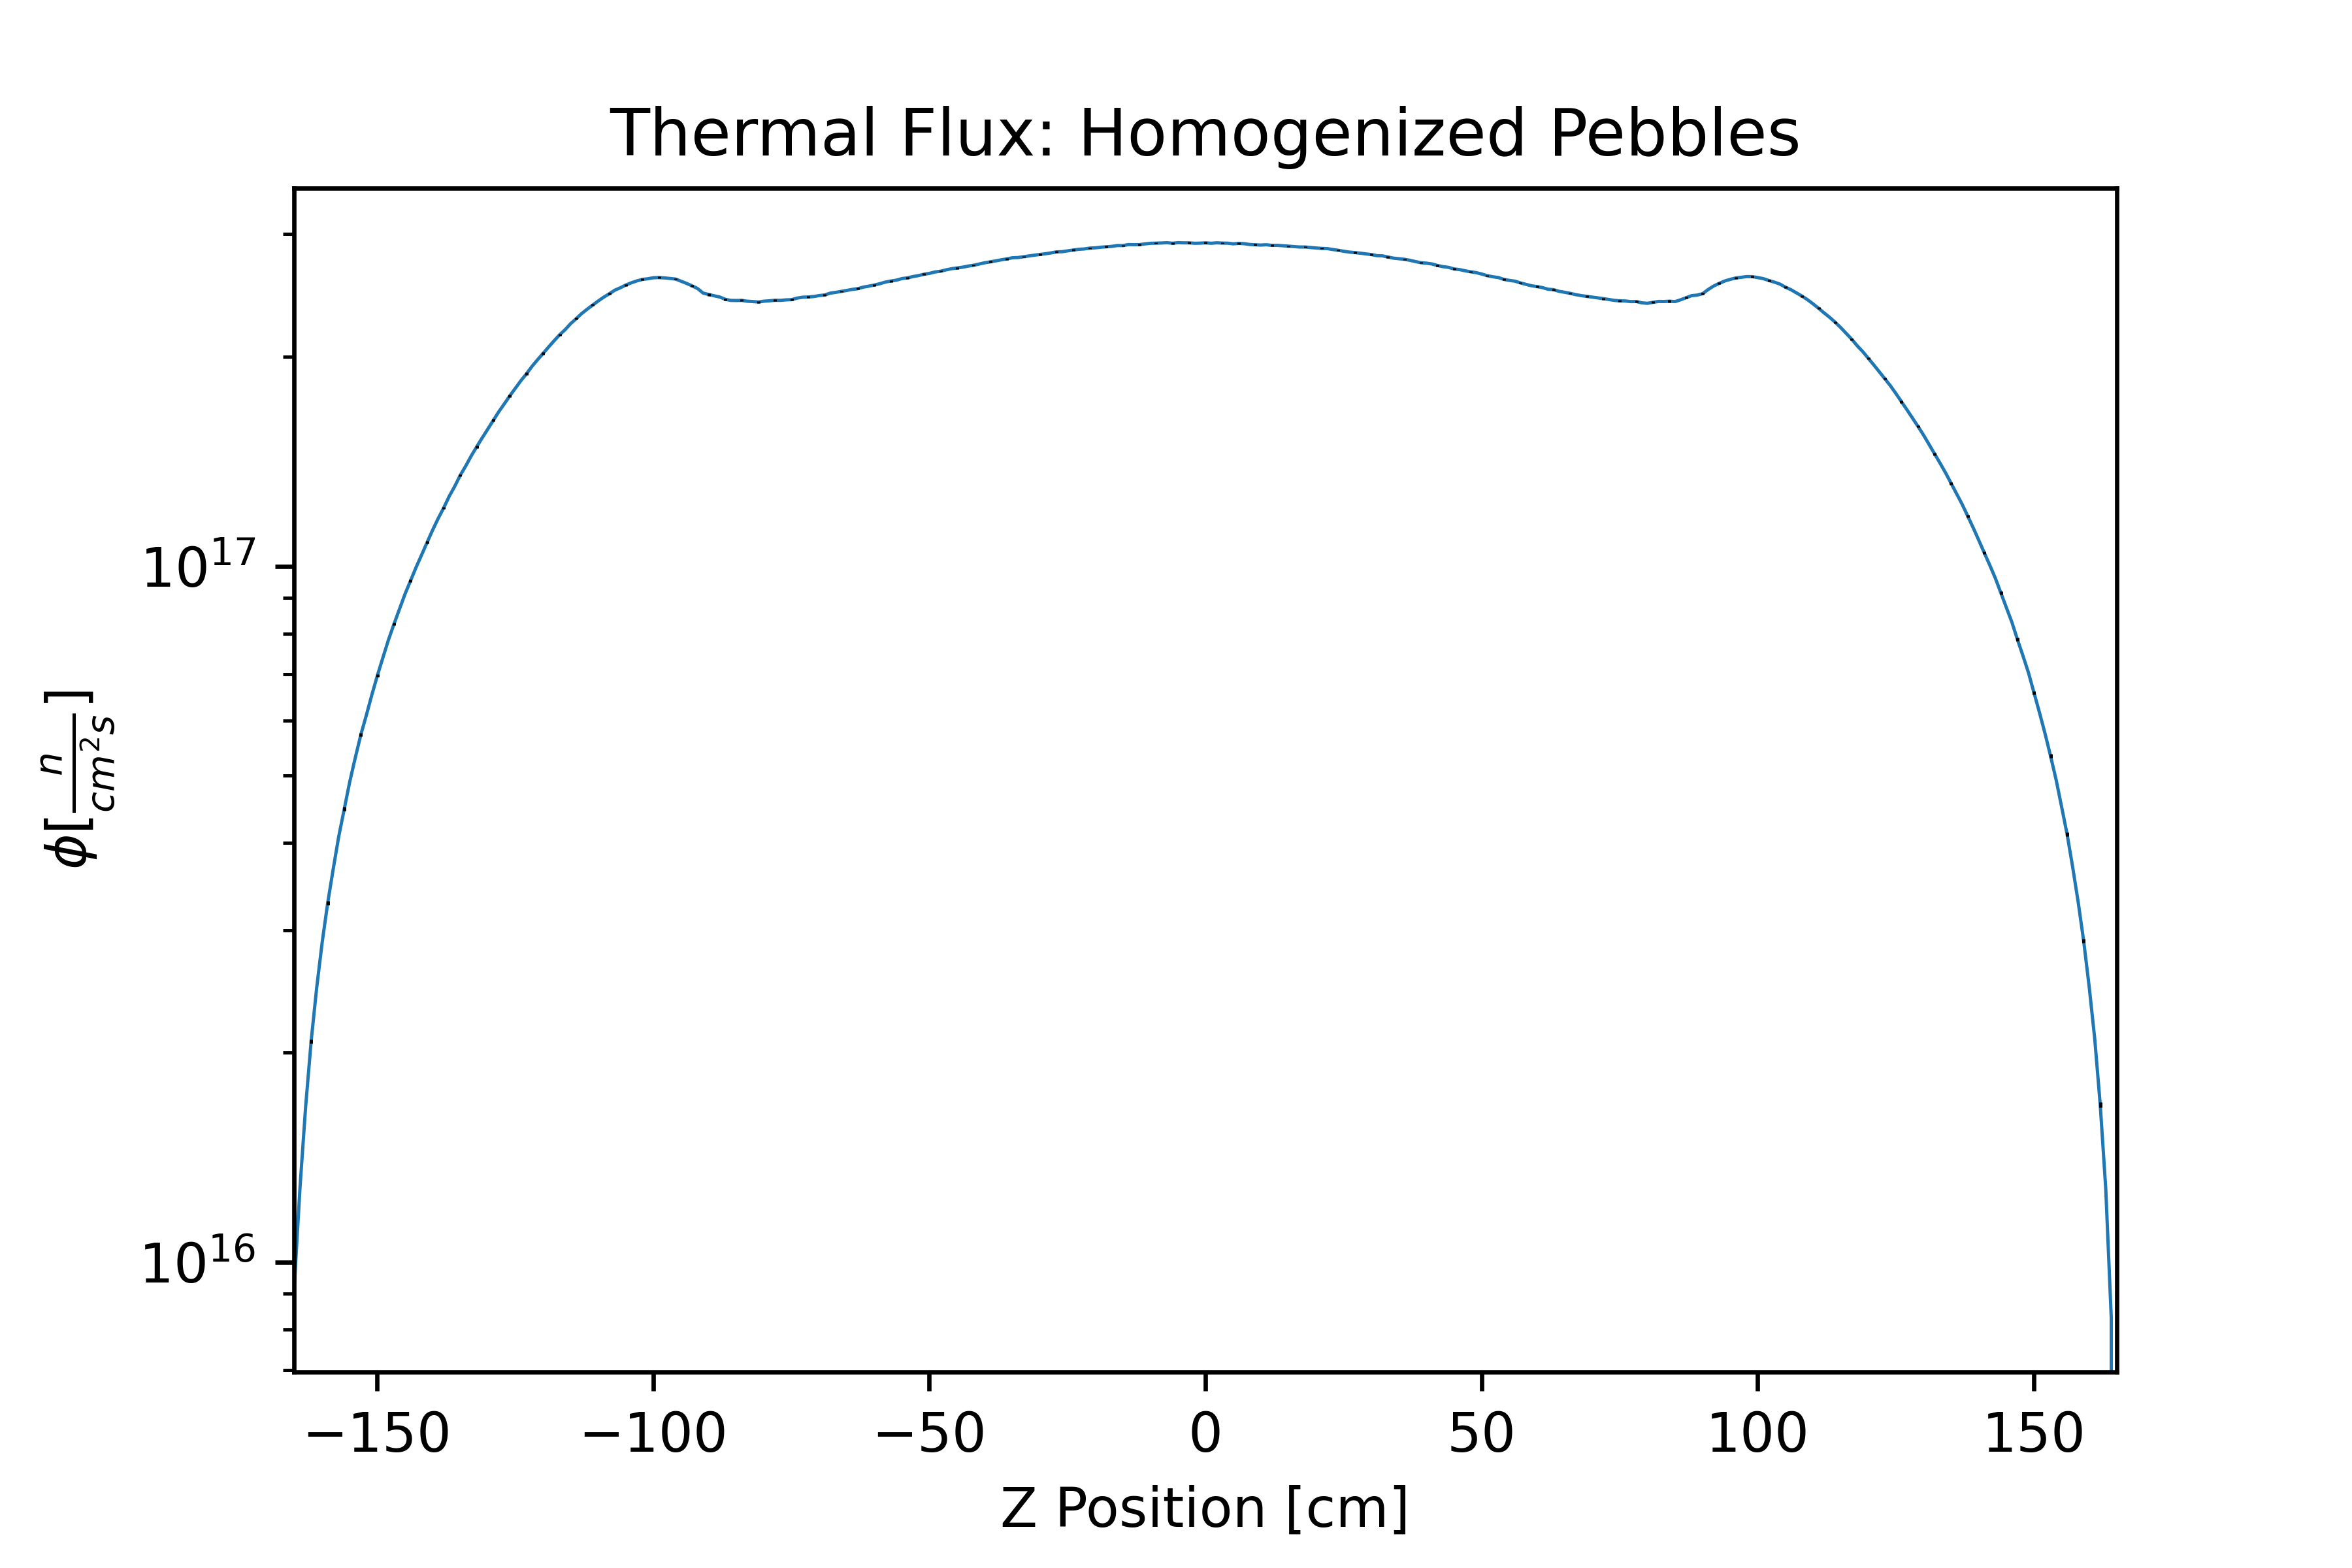
\includegraphics[width=0.95\linewidth]{figures/therm_flux_homog_z.png}
  \caption{Thermal Flux}
  \label{fig:hom-det-z-therm}
\end{subfigure}%
%
\begin{subfigure}{0.6\textwidth}
  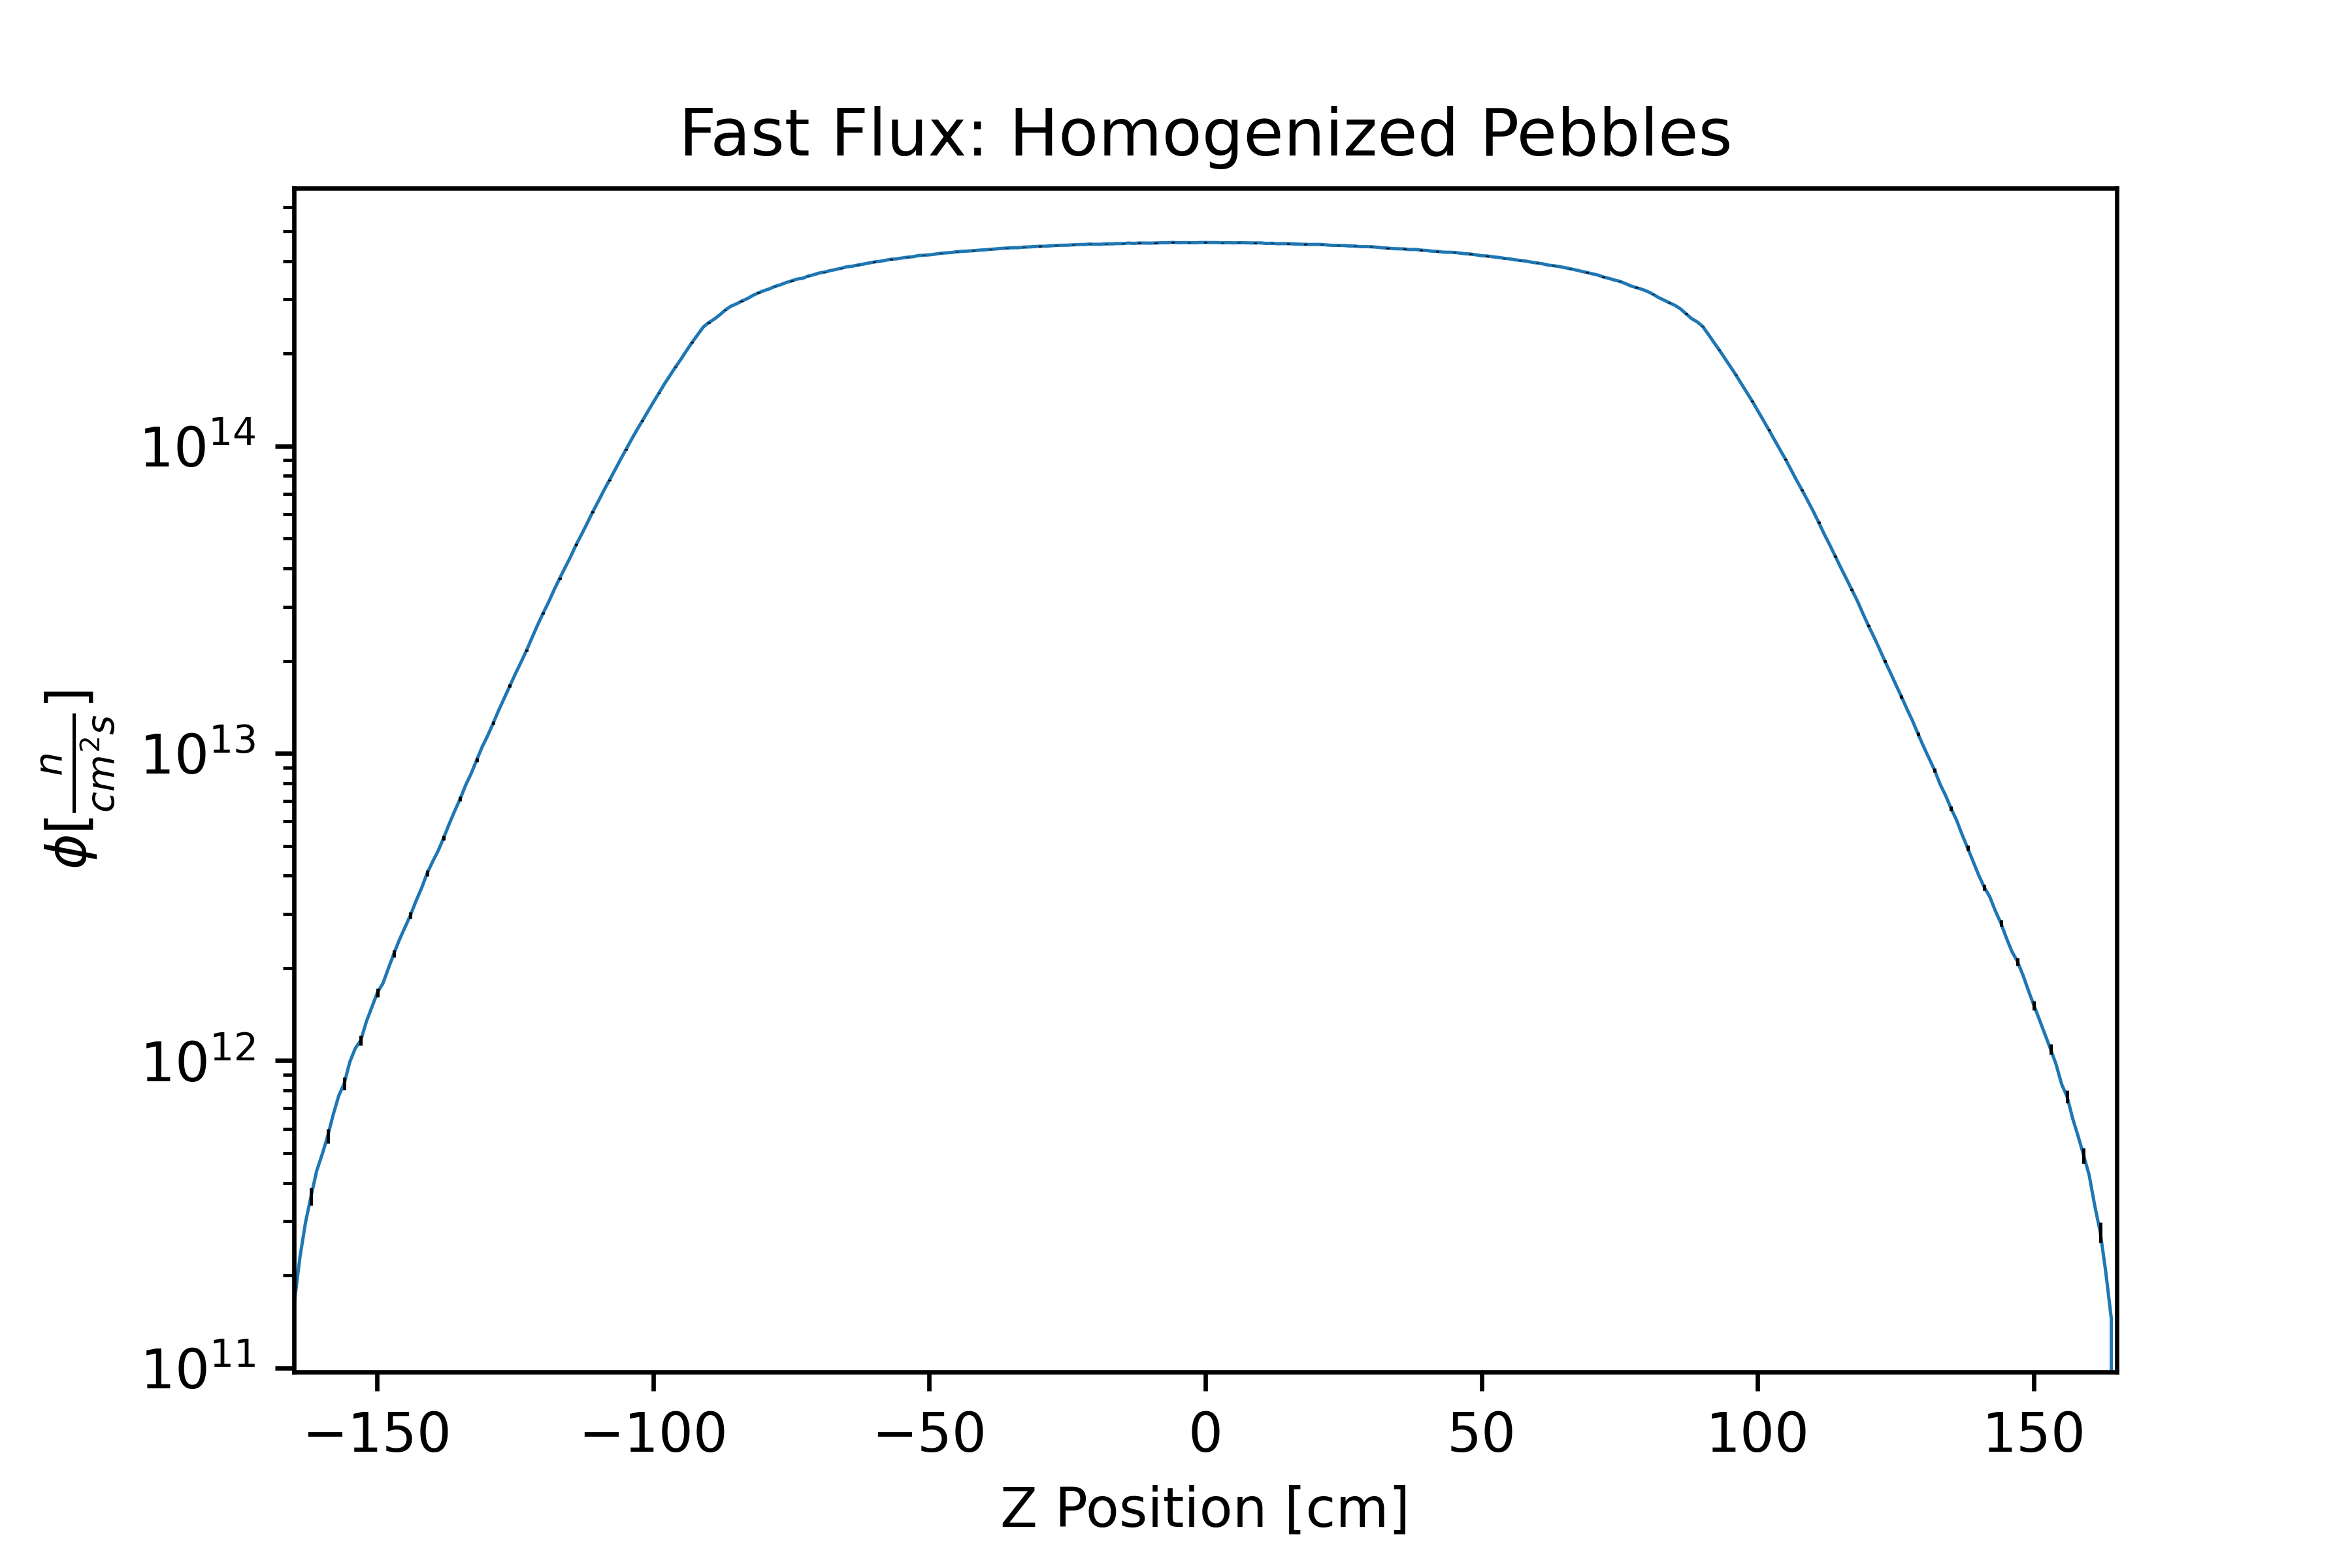
\includegraphics[width=0.95\linewidth]{figures/fast_flux_homog_z.png}
  \caption{Fast Flux}
  \label{fig:hom-det-z-fast}
\end{subfigure}

%
\caption{Axial Thermal and Fast Flux Profiles}
\label{fig:hom-det-z}
\end{figure}

***I know that there should be continuity at 0 between the axial and radial flux profiles, and there currently is a difference of 3 orders of magnitude.  I believe this is because of differing bin sizes between the detector that tracked the axial fluxes, and the detector that tracked the fluxes at the xy plane.  Basically, in the axial detector, each bin had a defined length in z, 0.1 cm or what-have-you.  However, these bins had no x or y limitations, and covered all x and y at that point (the bins are shaped like a stack of pancakes or such).  For the radial detector, I had to create the detector bins such that they formed a uniform grid over the xy plane, centered on the origin (which is the physical center of the reactor).  These bins were finite in x and y, but not in the z direction, so they covered all z that fell within the limits of the bin (these bins are like a long rectangular prism).  While this uniform grid prevents the radial flux profile from warping, which is what happens if you attempt to make a detector along only one axis (the bins end up being unequal sizes), the fact that the axial detector bins differ from the radial detector bins means they don't match each other.

tl;dr: should I divide the neutron flux by bin volume so the axial and radial profiles match in magnitude (hopefully)***

Figures \ref{fig:hom-det-xy} and \ref{fig:hom-det-z} provide the fast and thermal flux profiles in Sangamon20.  The former are the radial fluxes, along the x-axis, and the latter are the axial center line ***can I just say center line?*** profiles.  Both axially and radially, the thermal flux sees a 'bump', which peaks approximately 10 cm into the reflector, at 100 cm.  These are the highest peaks in the thermal flux, with the second highest thermal flux being at the center line.  For the fast flux profile, we see a flattened peak in the  active core (-90.0 cm to 90 cm) and 10 cm into the reflector.  Fast flux rapidly decreases in the reflector, as fast neutrons down scatter in the graphite.

Both \ref{fig:hom-det-xy} and \ref{fig:hom-det-z} show that the radial banding seen in the fission rate mesh profiles, which appear to be of a very high intensity, are not actually where the true peaks in the flux profiles are located.


\begin{figure}[H]
\centering

  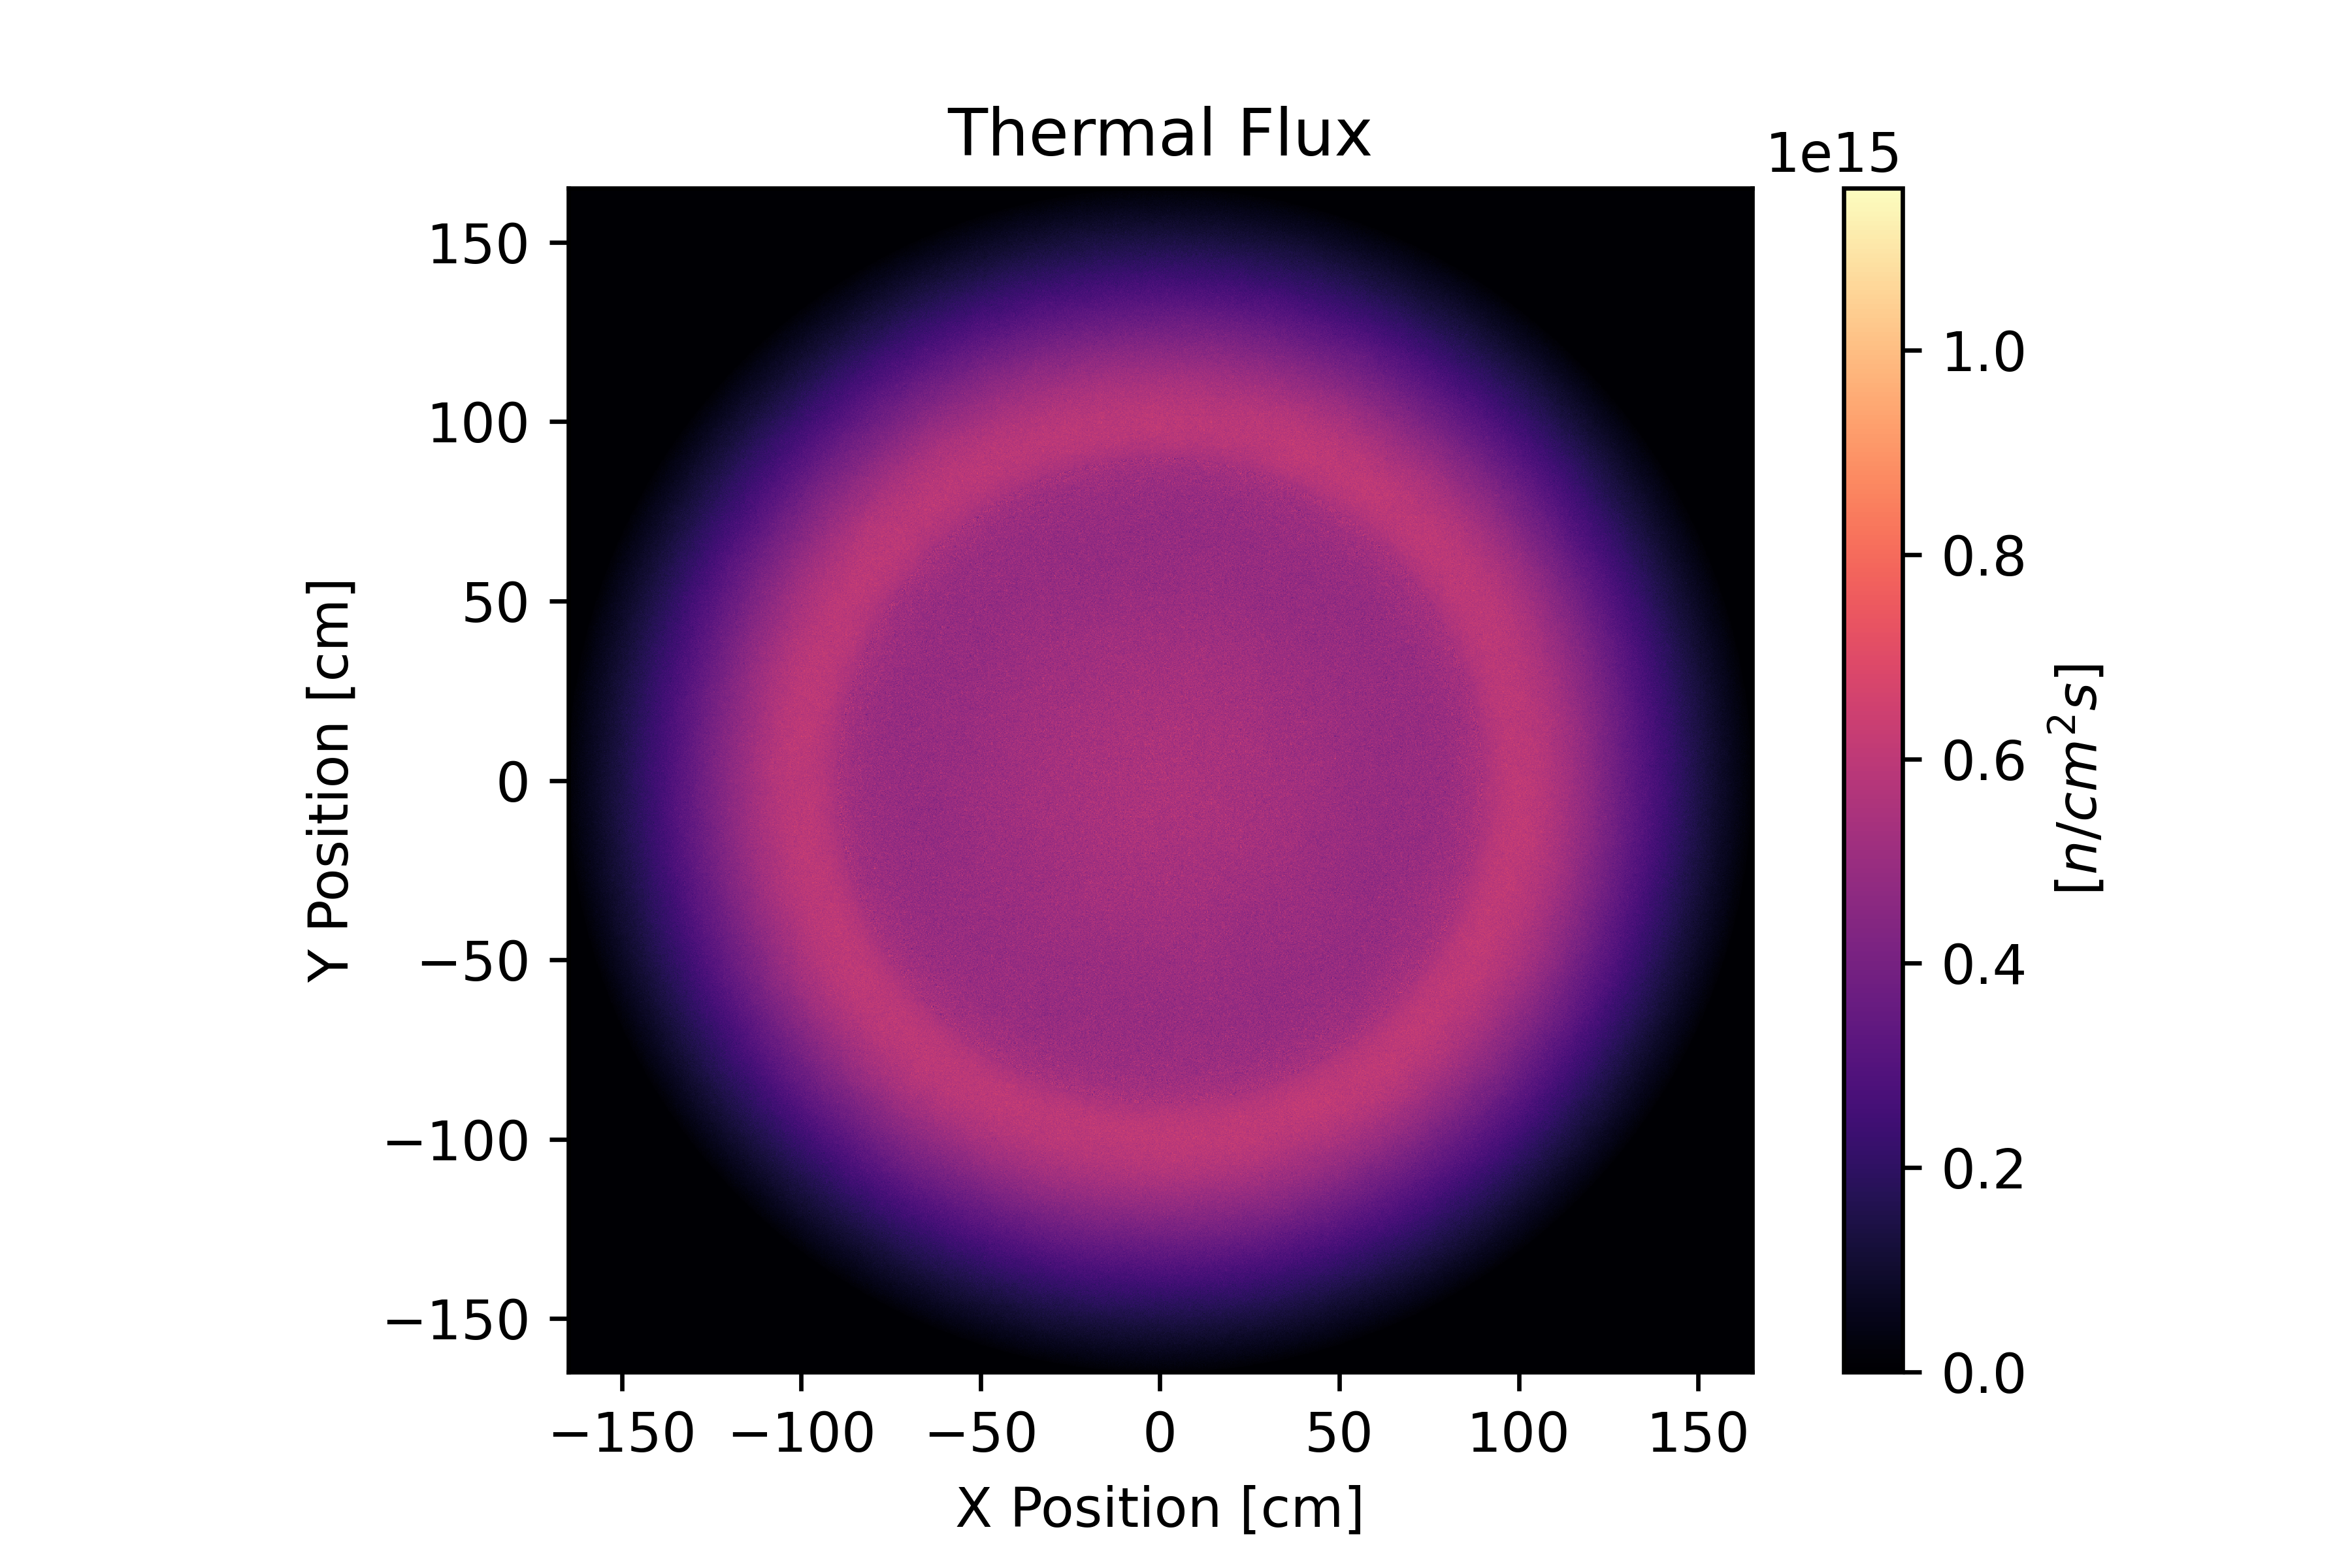
\includegraphics[width=1.0\linewidth]{figures/therm_xy_plane_homog_er.png}
  \caption{Thermal Flux in xy Plane in Sangamon20: Homogenized Pebbles.  The dotted line annotation marks the boundary between the active core and the graphite reflector.}
  \label{fig:hom-plane-therm}

\end{figure}


\begin{figure}[H]
\centering

 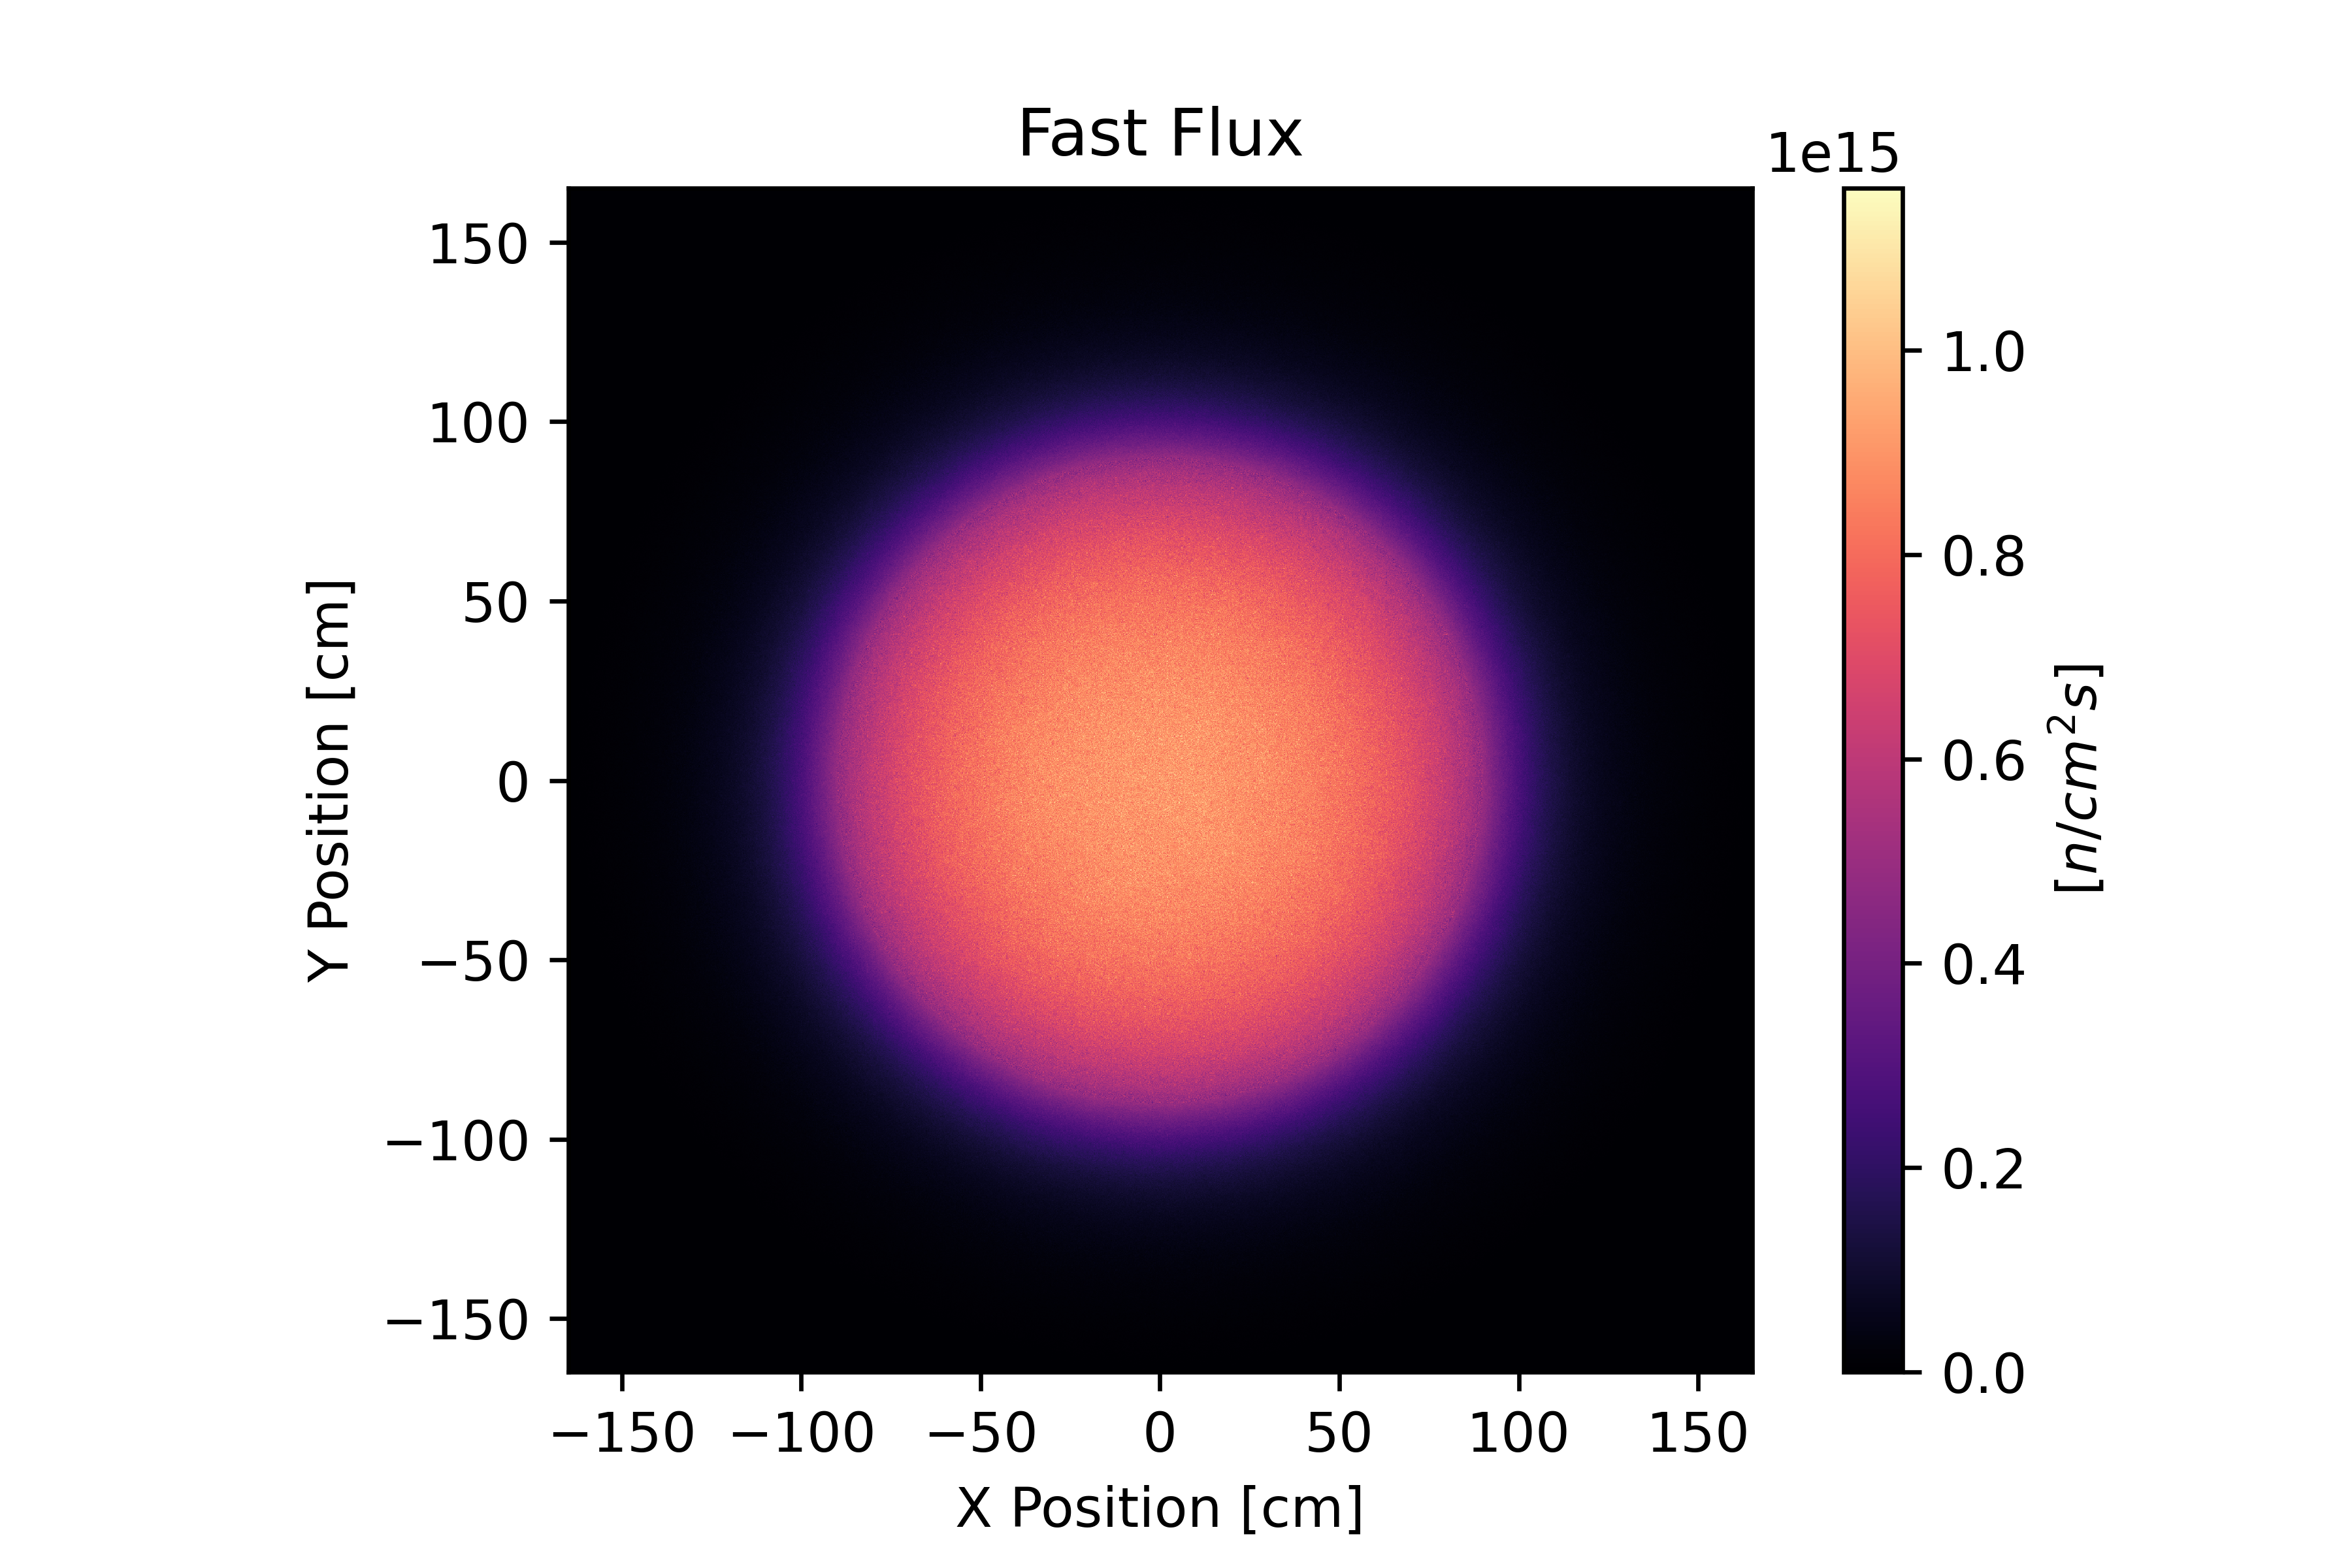
\includegraphics[width=1.0\linewidth]{figures/fast_xy_plane_homog_er.png}
 \caption{Fast Flux in xy Plane in Sangamon20: Homogenized Pebbles.  The dotted line annotation marks the boundary between the active core and the graphite reflector.}
 \label{fig:hom-plane-fast}

\end{figure}

***okay, these mesh figures in particular I A) have a lot of trouble getting to a good size and B) kinda want to make big to see detail (especially since I discuss some of the finer details in the image).  Maybe I could show a smaller version here, and then add a larger version in the appendix, where it doesn't matter if my mesh plot takes up its own page. ***

Figure \ref{fig:hom-det-plane} provides the total flux over the xy plane at z = 0.  A slight banding pattern on the active core's edge can be seen, but not with the same intensity of the fission rate banding.  Once again, figure \ref{fig:hom-det-plane} shows that while the banding morphology may be present in the flux profile (and do cause a slight increase relative to the region immediately surrounding it) it does not cause large concentric spikes in the flux profiles.

\begin{figure}[h!]
\centering
%
\begin{subfigure}{0.25\textwidth}
  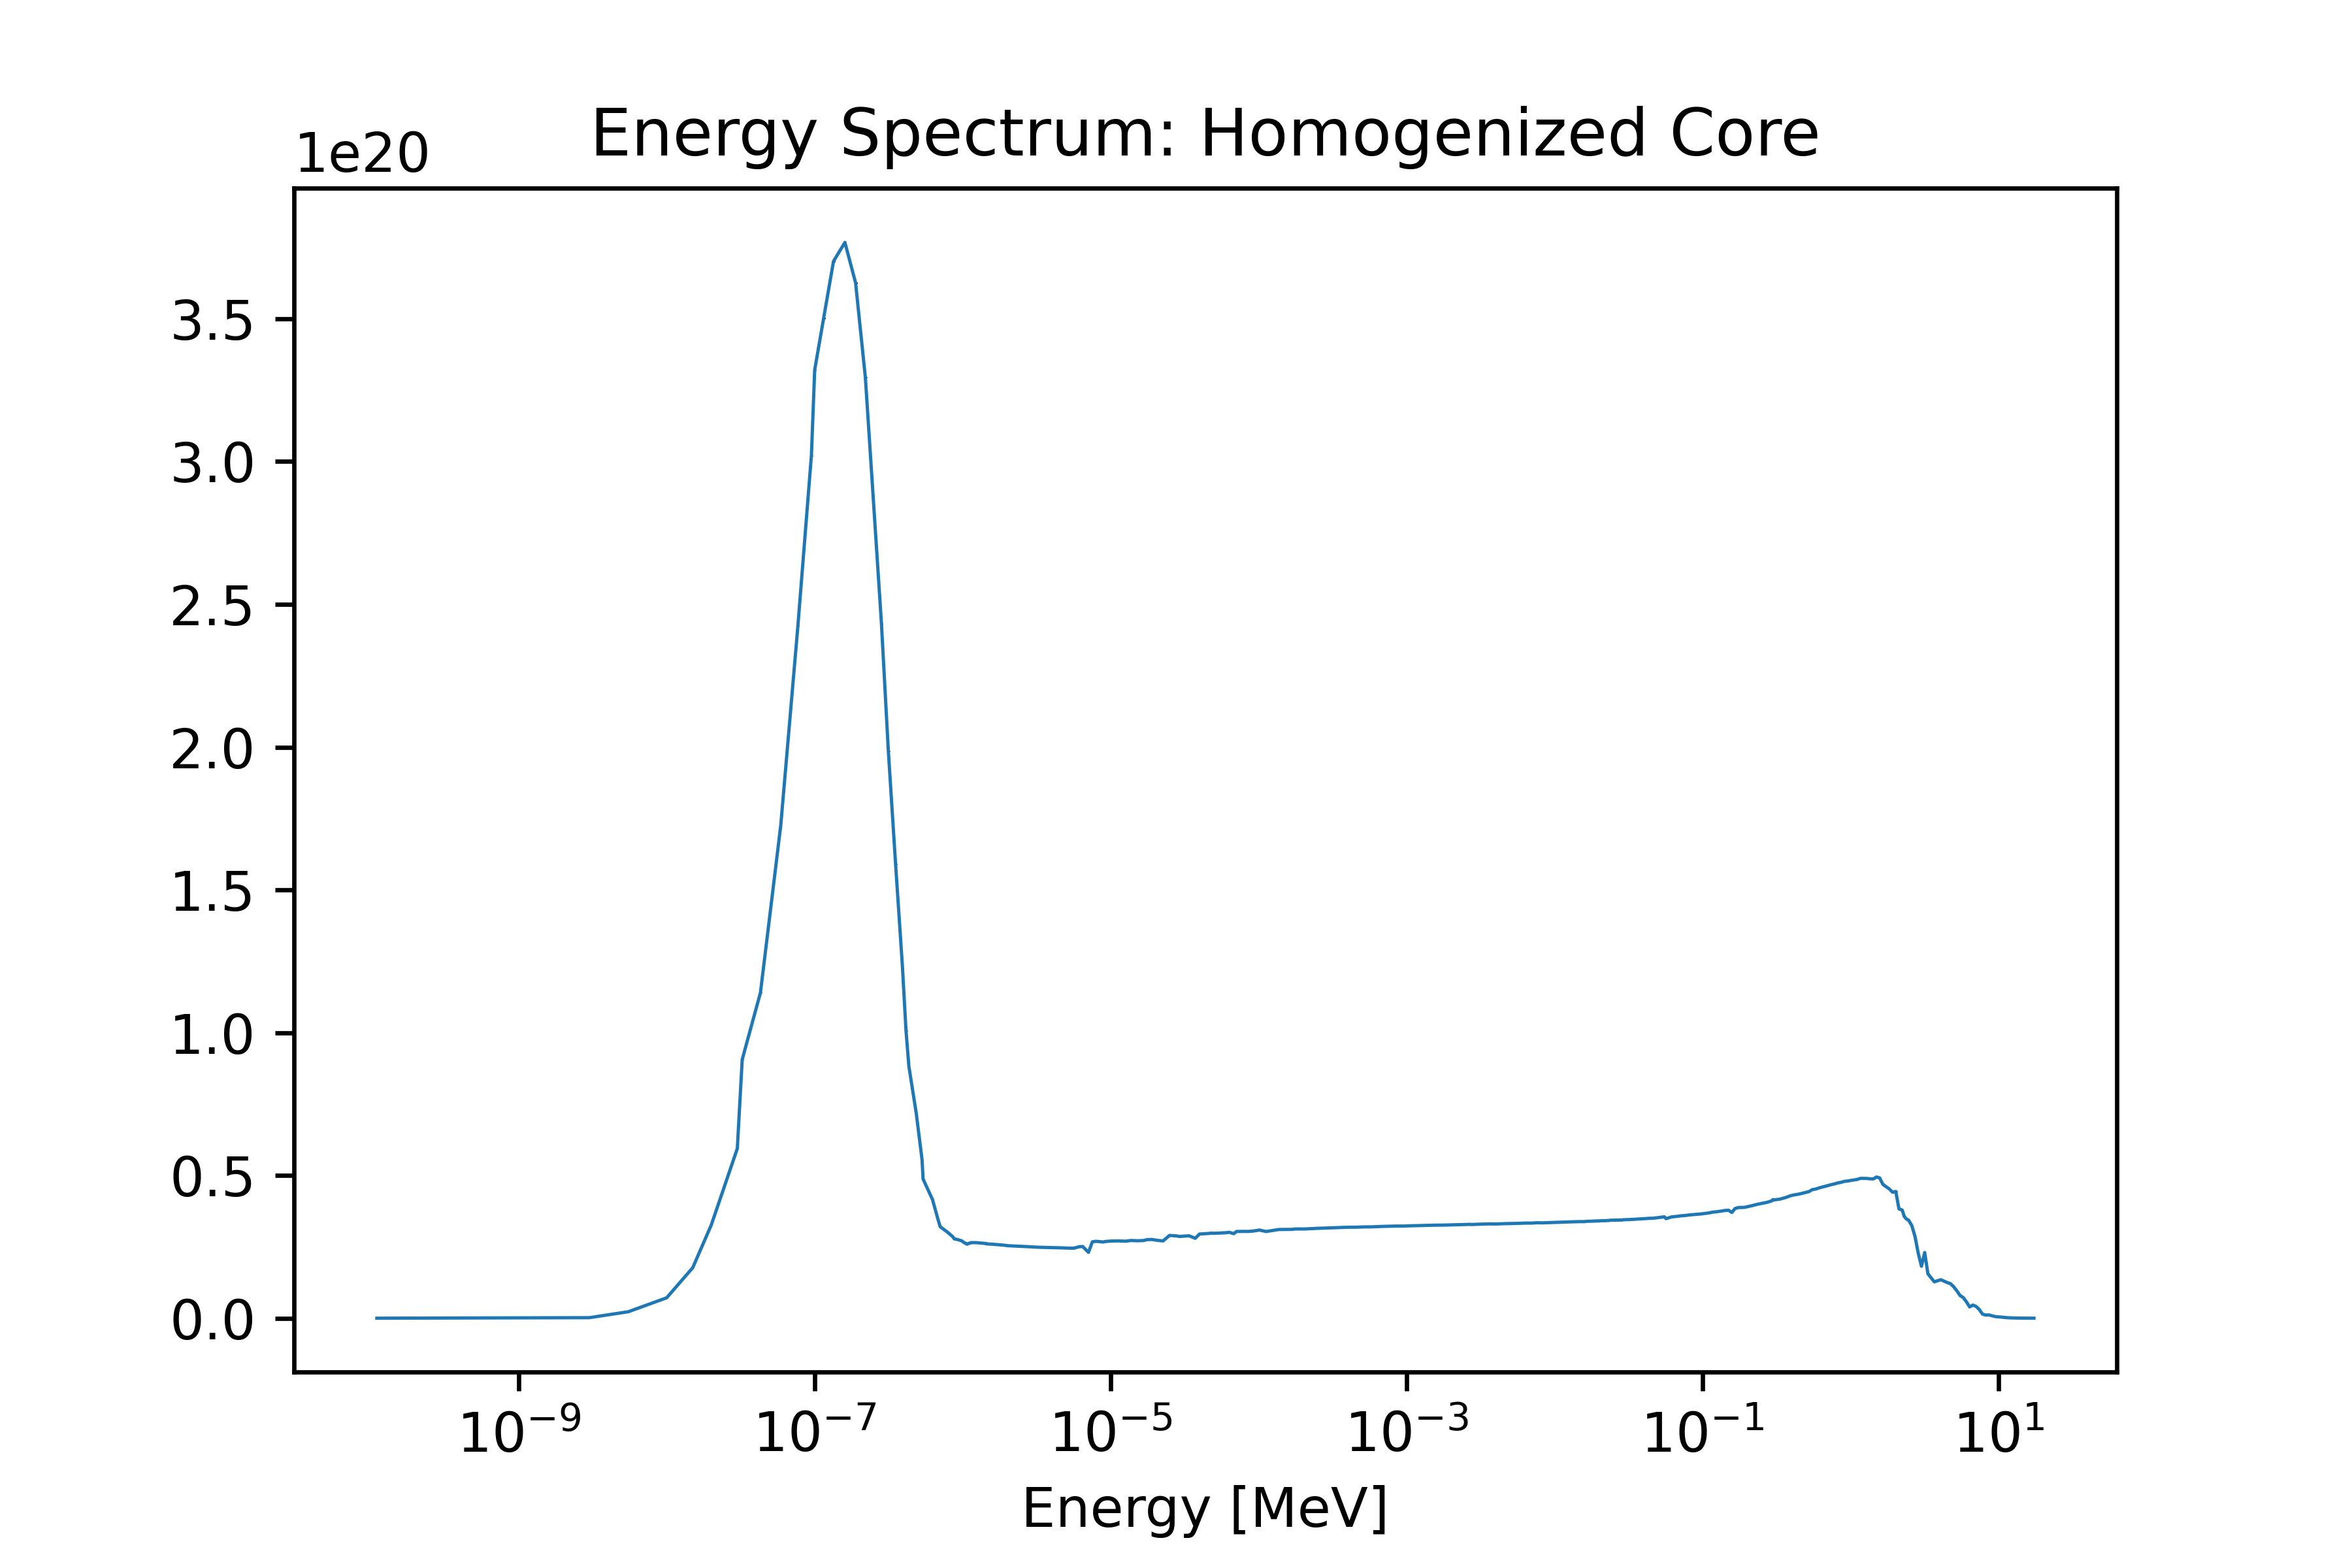
\includegraphics[width=0.95\linewidth]{figures/core_spec_homog}
  \caption{Core Spectrum}
  \label{fig:hom-core}
\end{subfigure}%
%
\begin{subfigure}{0.25\textwidth}
  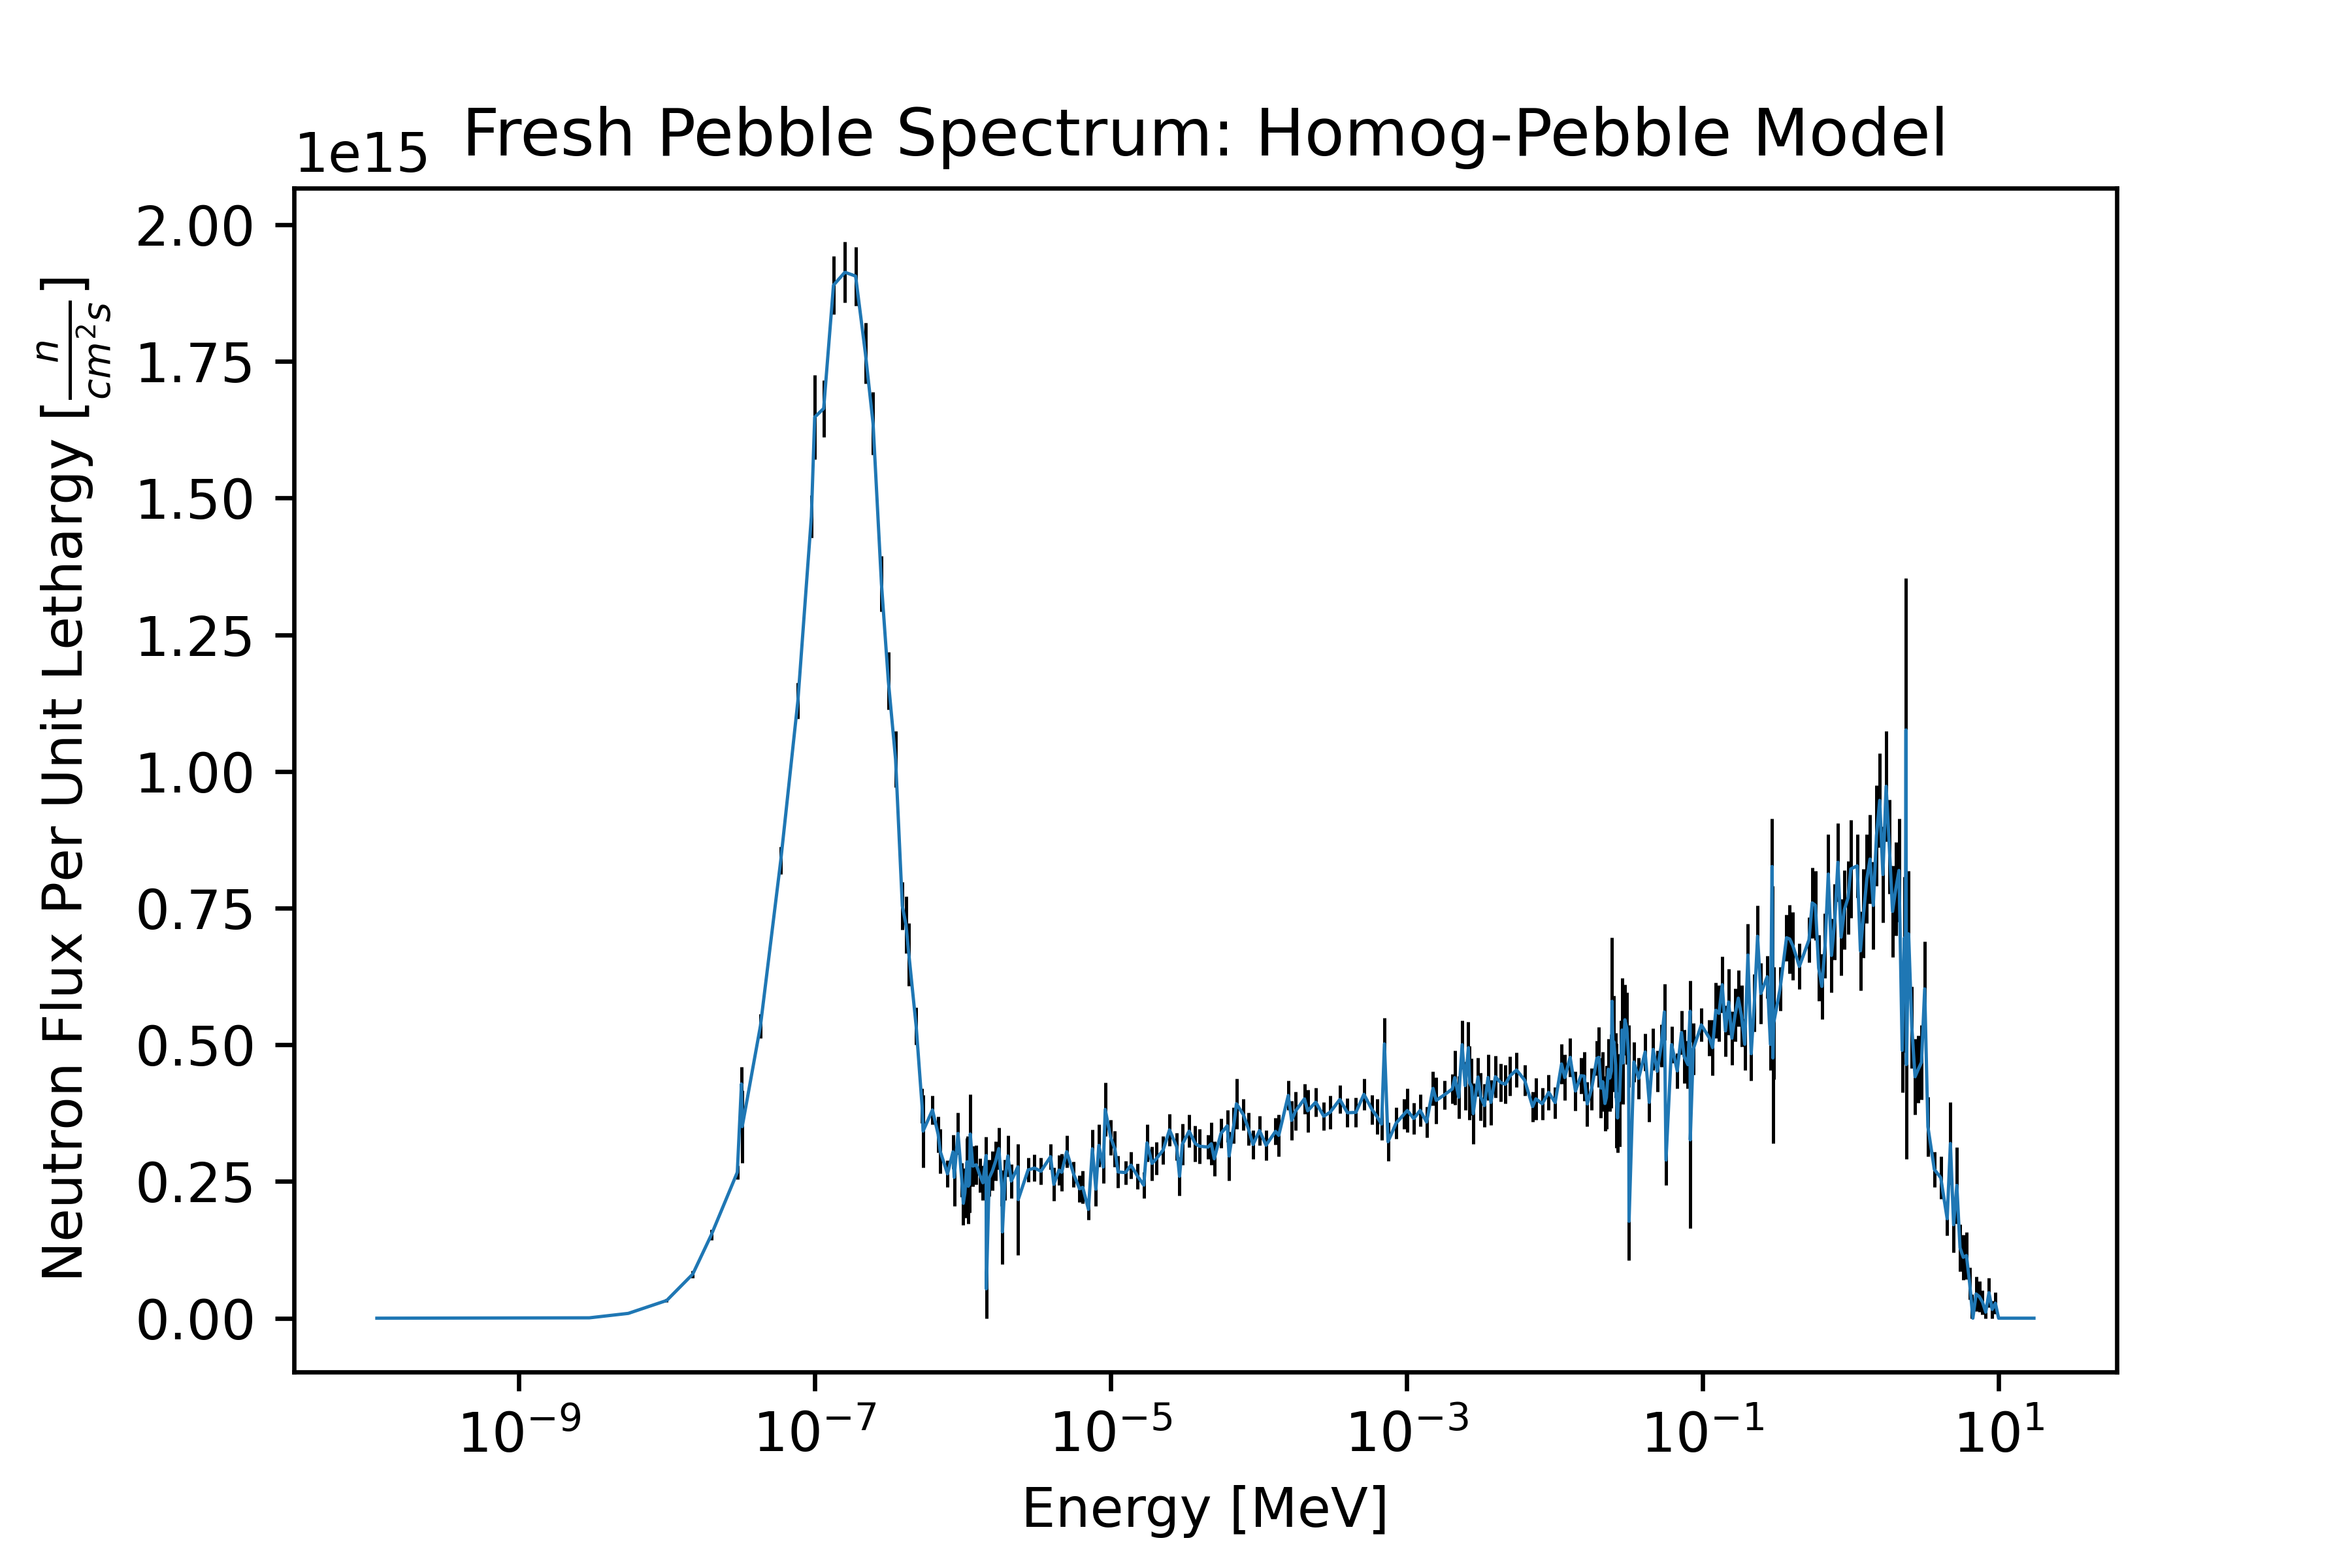
\includegraphics[width=0.95\linewidth]{figures/fresh_spec_homog}
  \caption{Fresh Pebble Spectrum}
  \label{fig:hom-fresh}
\end{subfigure}%
%
\begin{subfigure}{0.25\textwidth}
  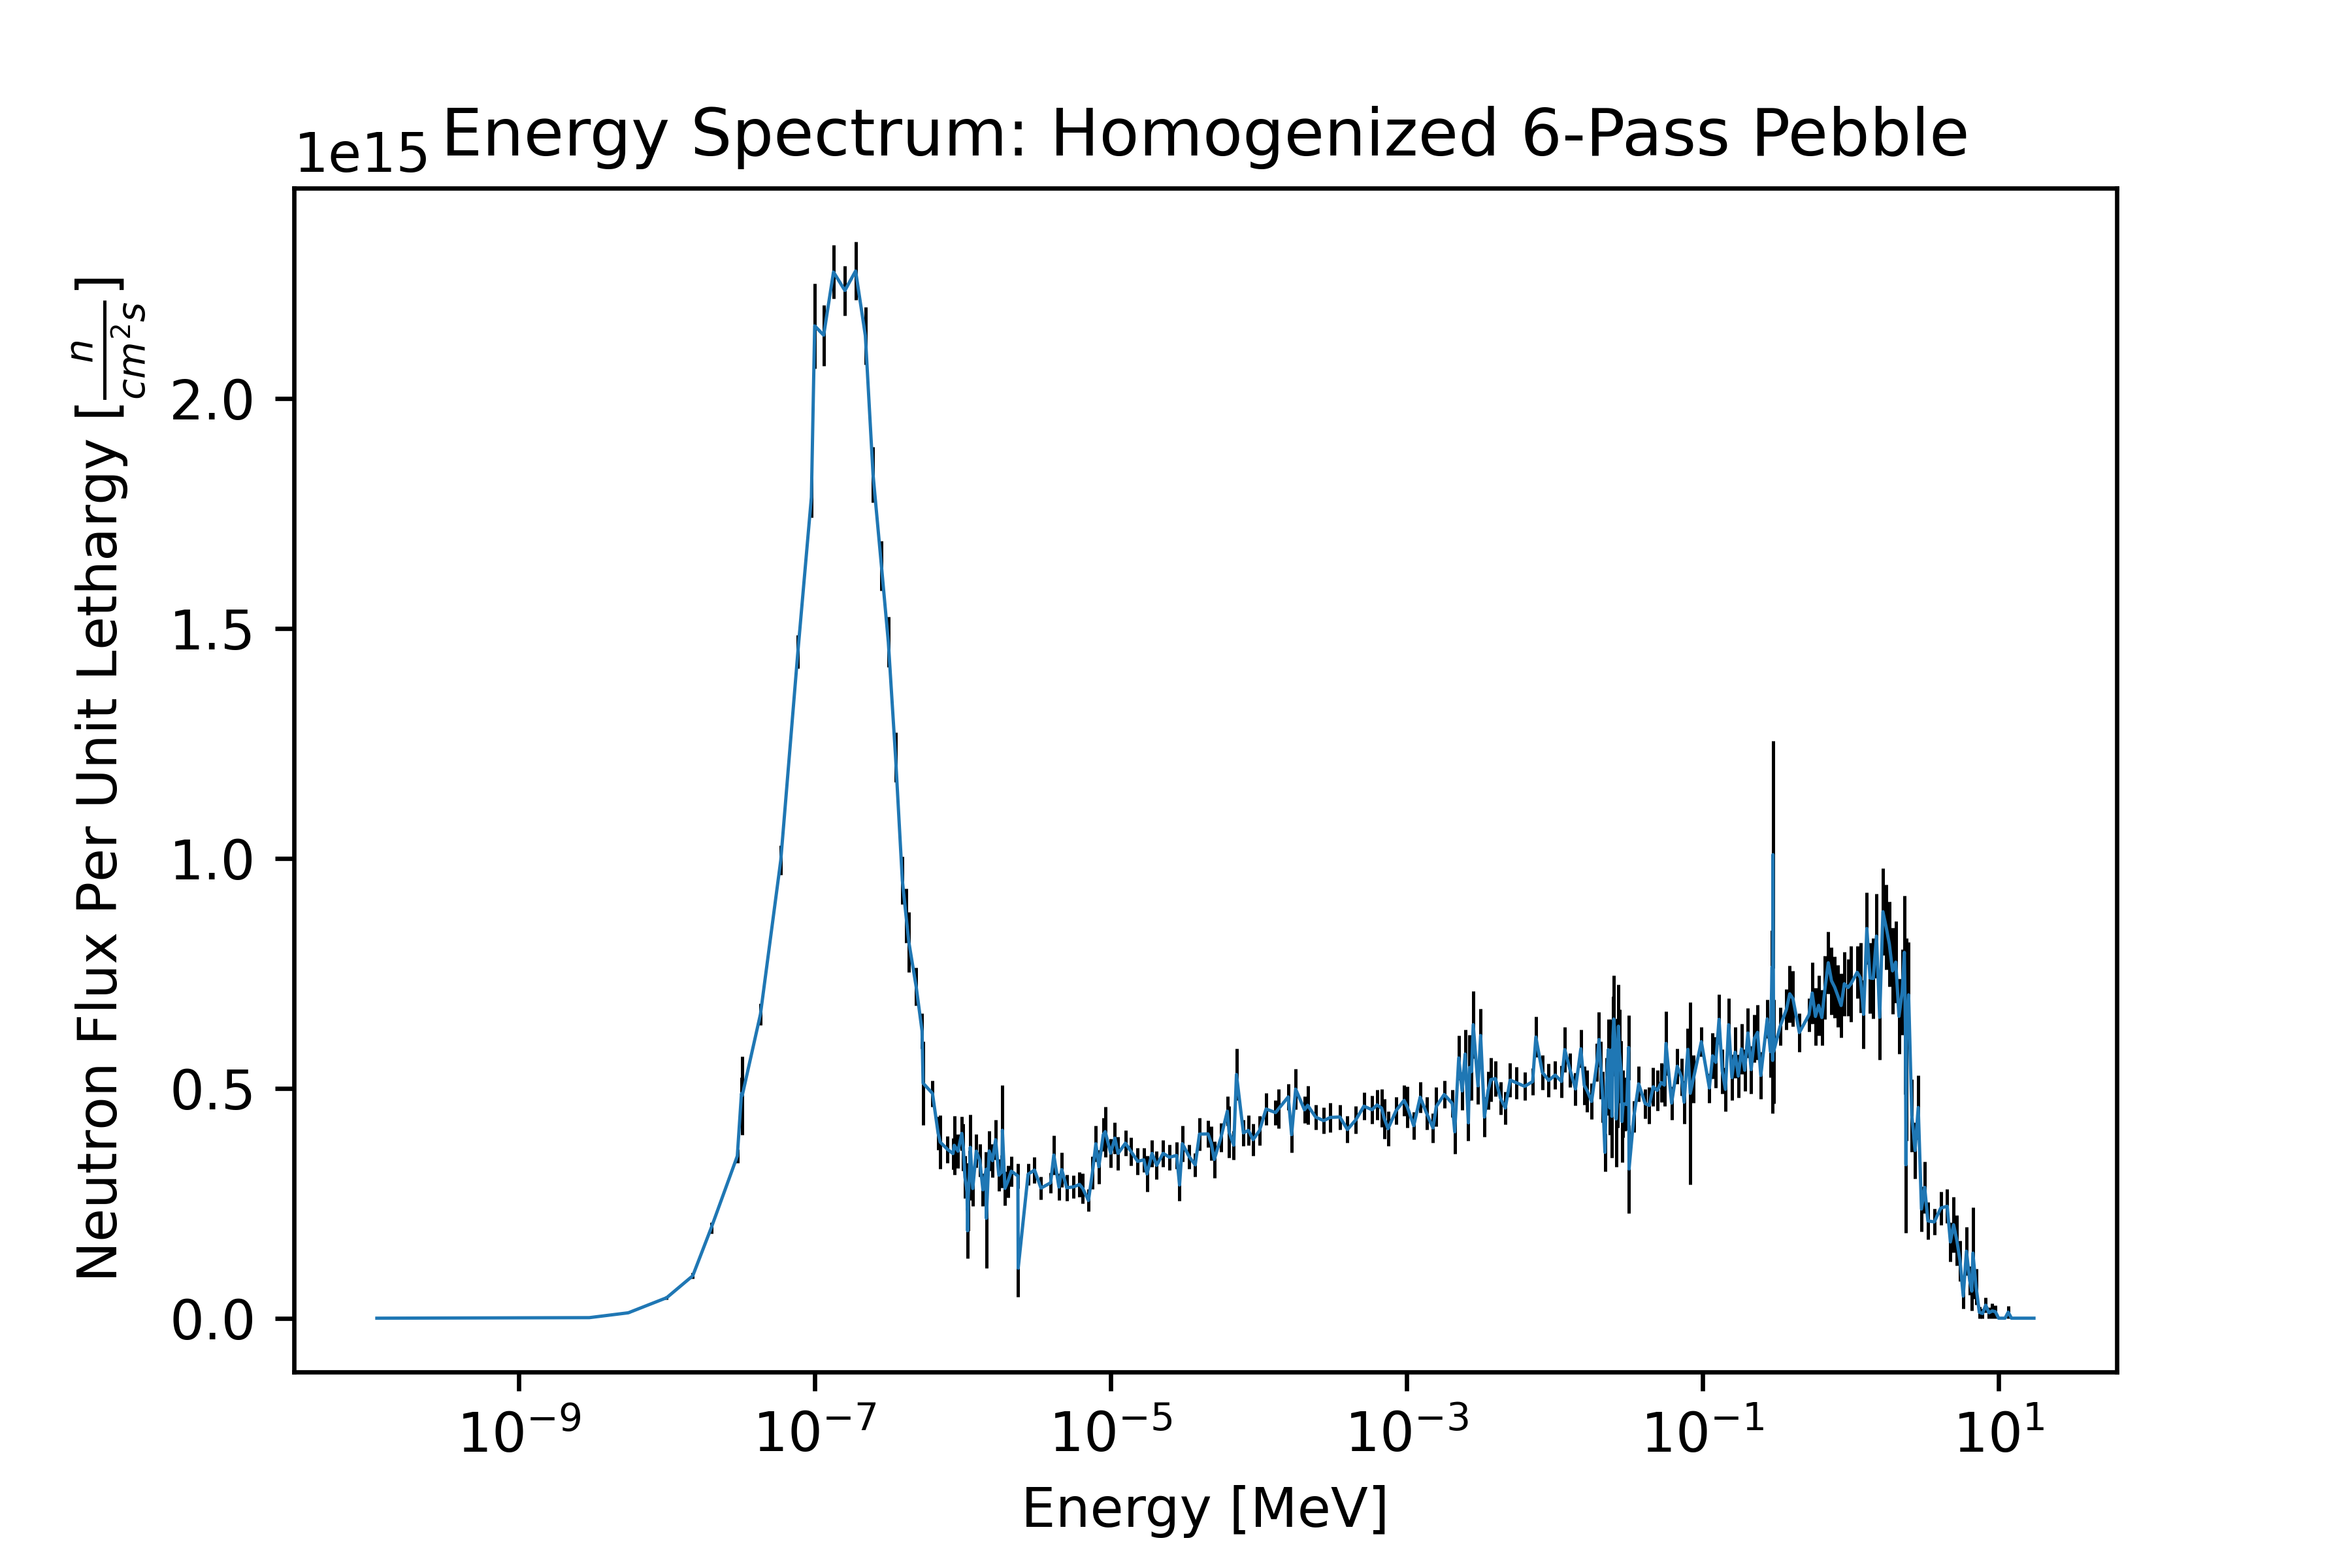
\includegraphics[width=0.95\linewidth]{figures/6_spec_homog}
  \caption{Six-Pass Pebble Spectrum}
  \label{fig:hom-six}
\end{subfigure}%

\begin{subfigure}{0.25\textwidth}
  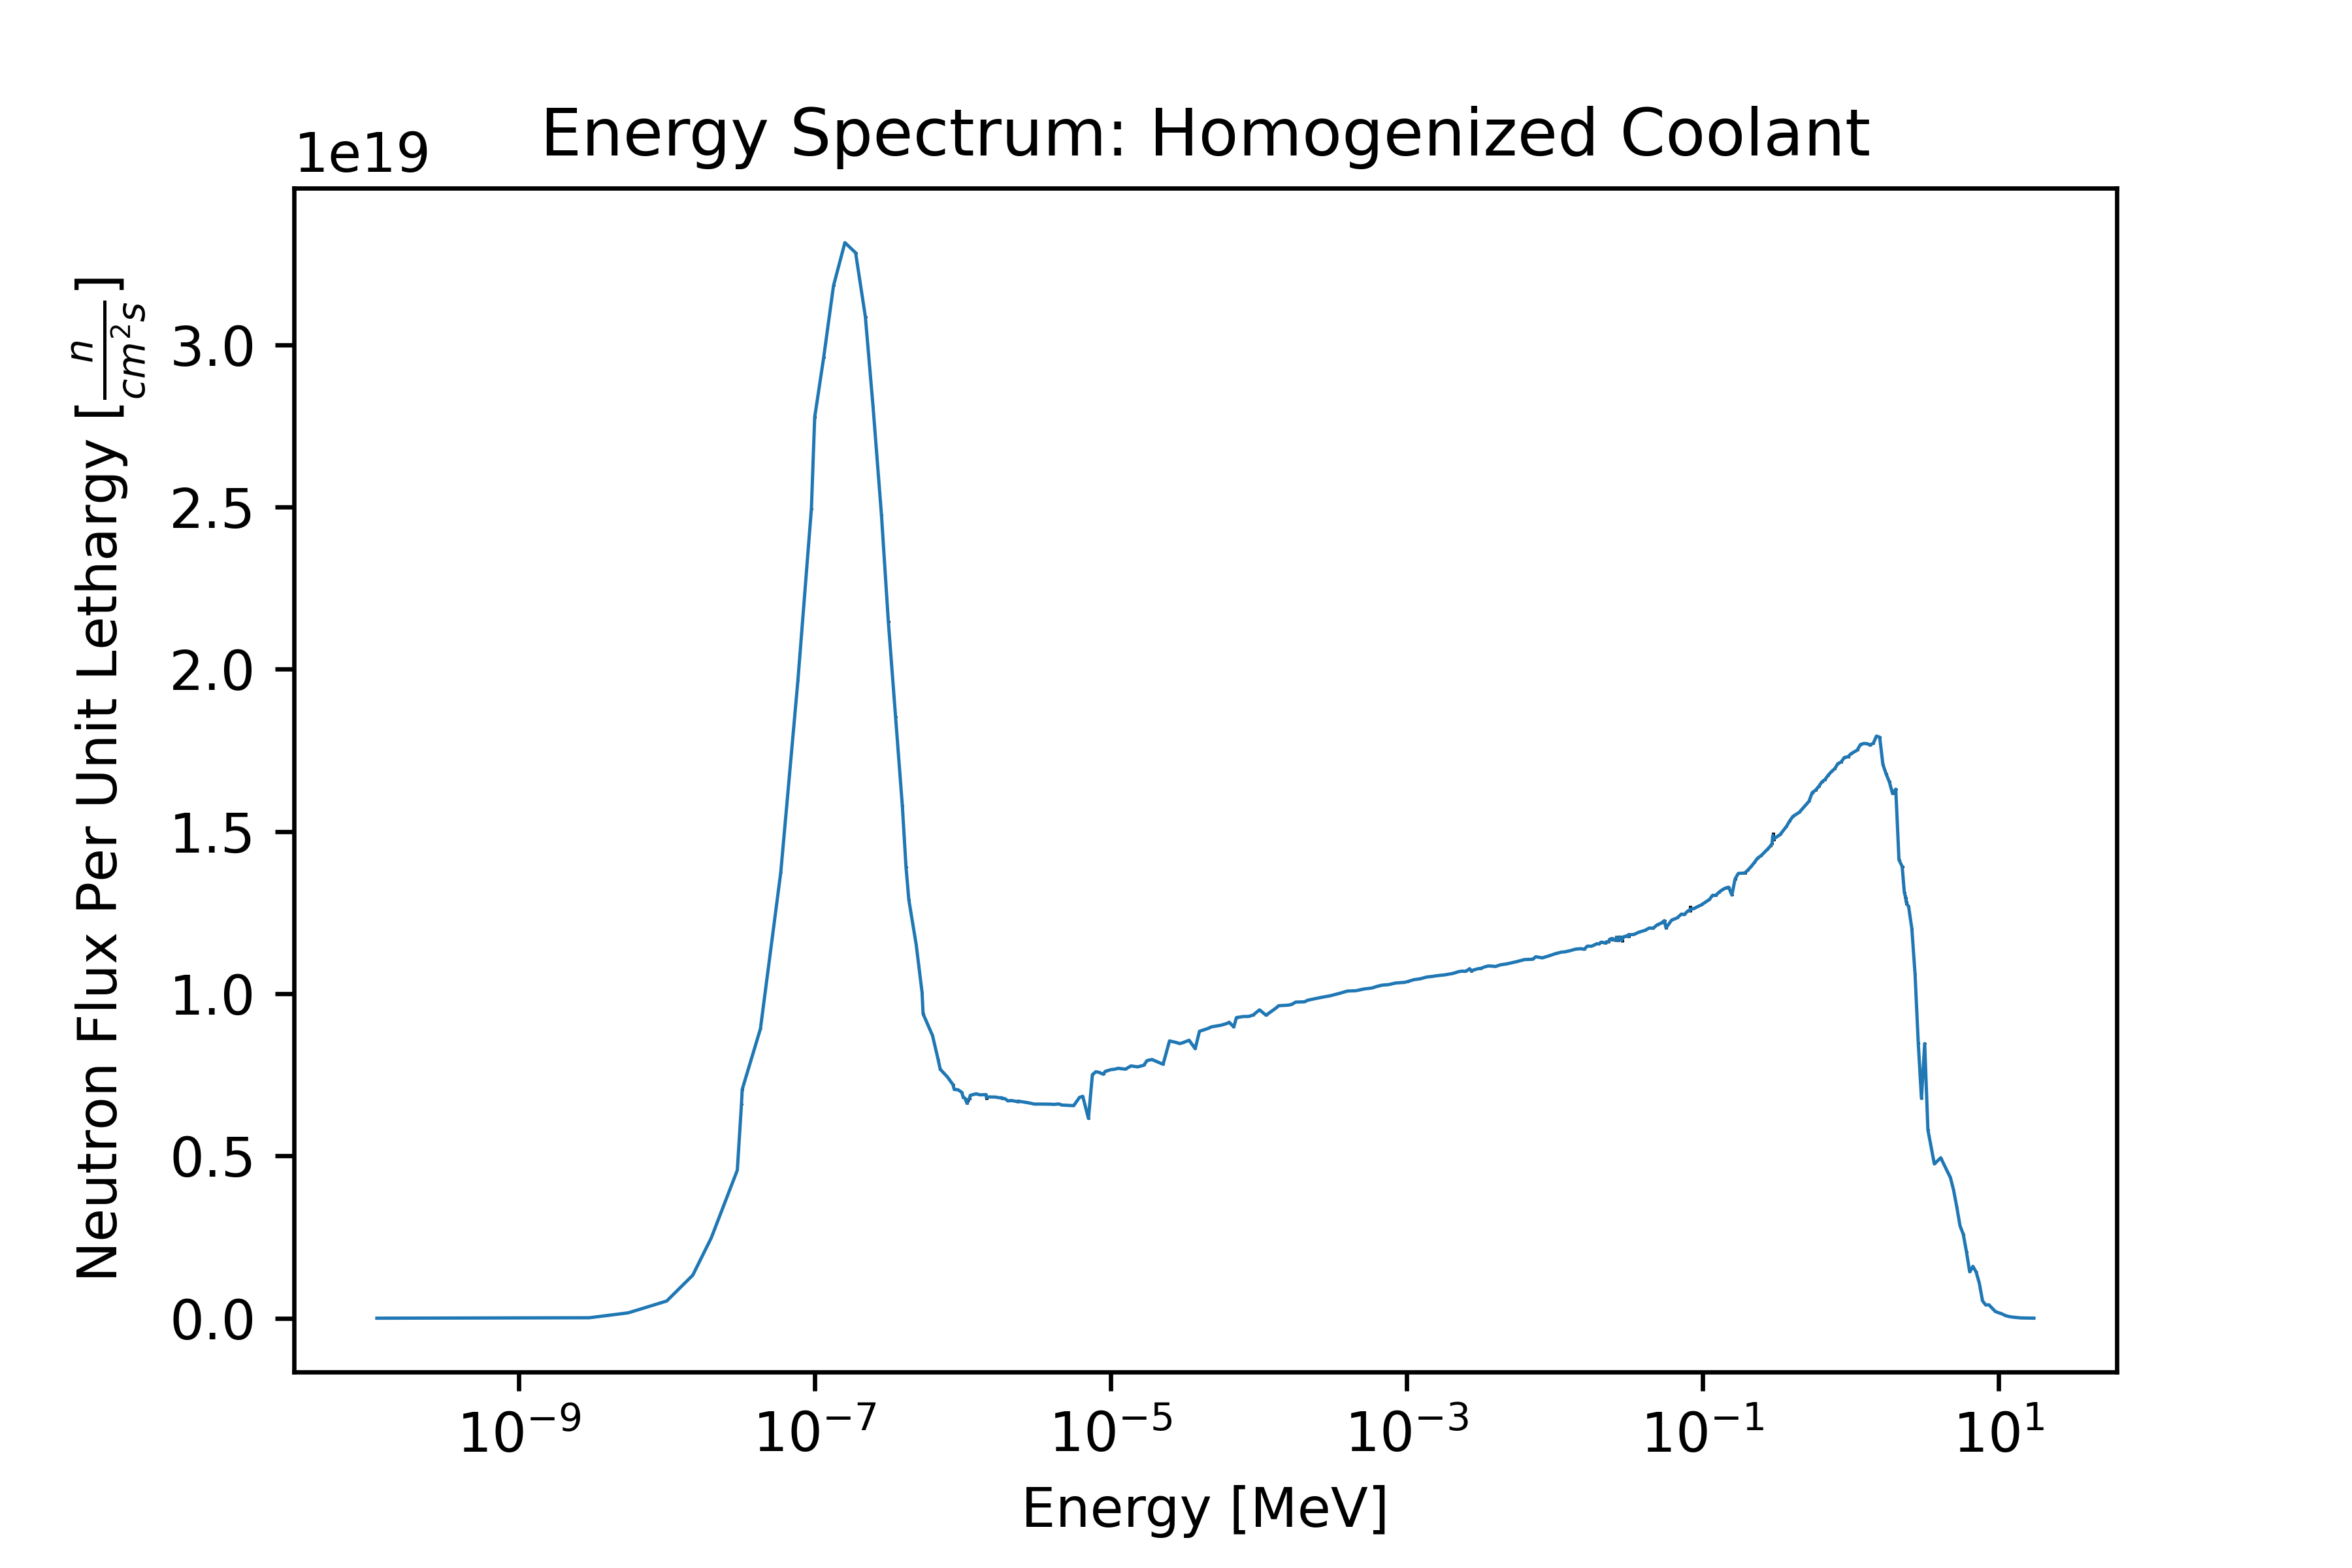
\includegraphics[width=0.95\linewidth]{figures/cool_spec_homog}
  \caption{Coolant Spectrum}
  \label{fig:hom-cool}
\end{subfigure}%
%
\begin{subfigure}{0.25\textwidth}
  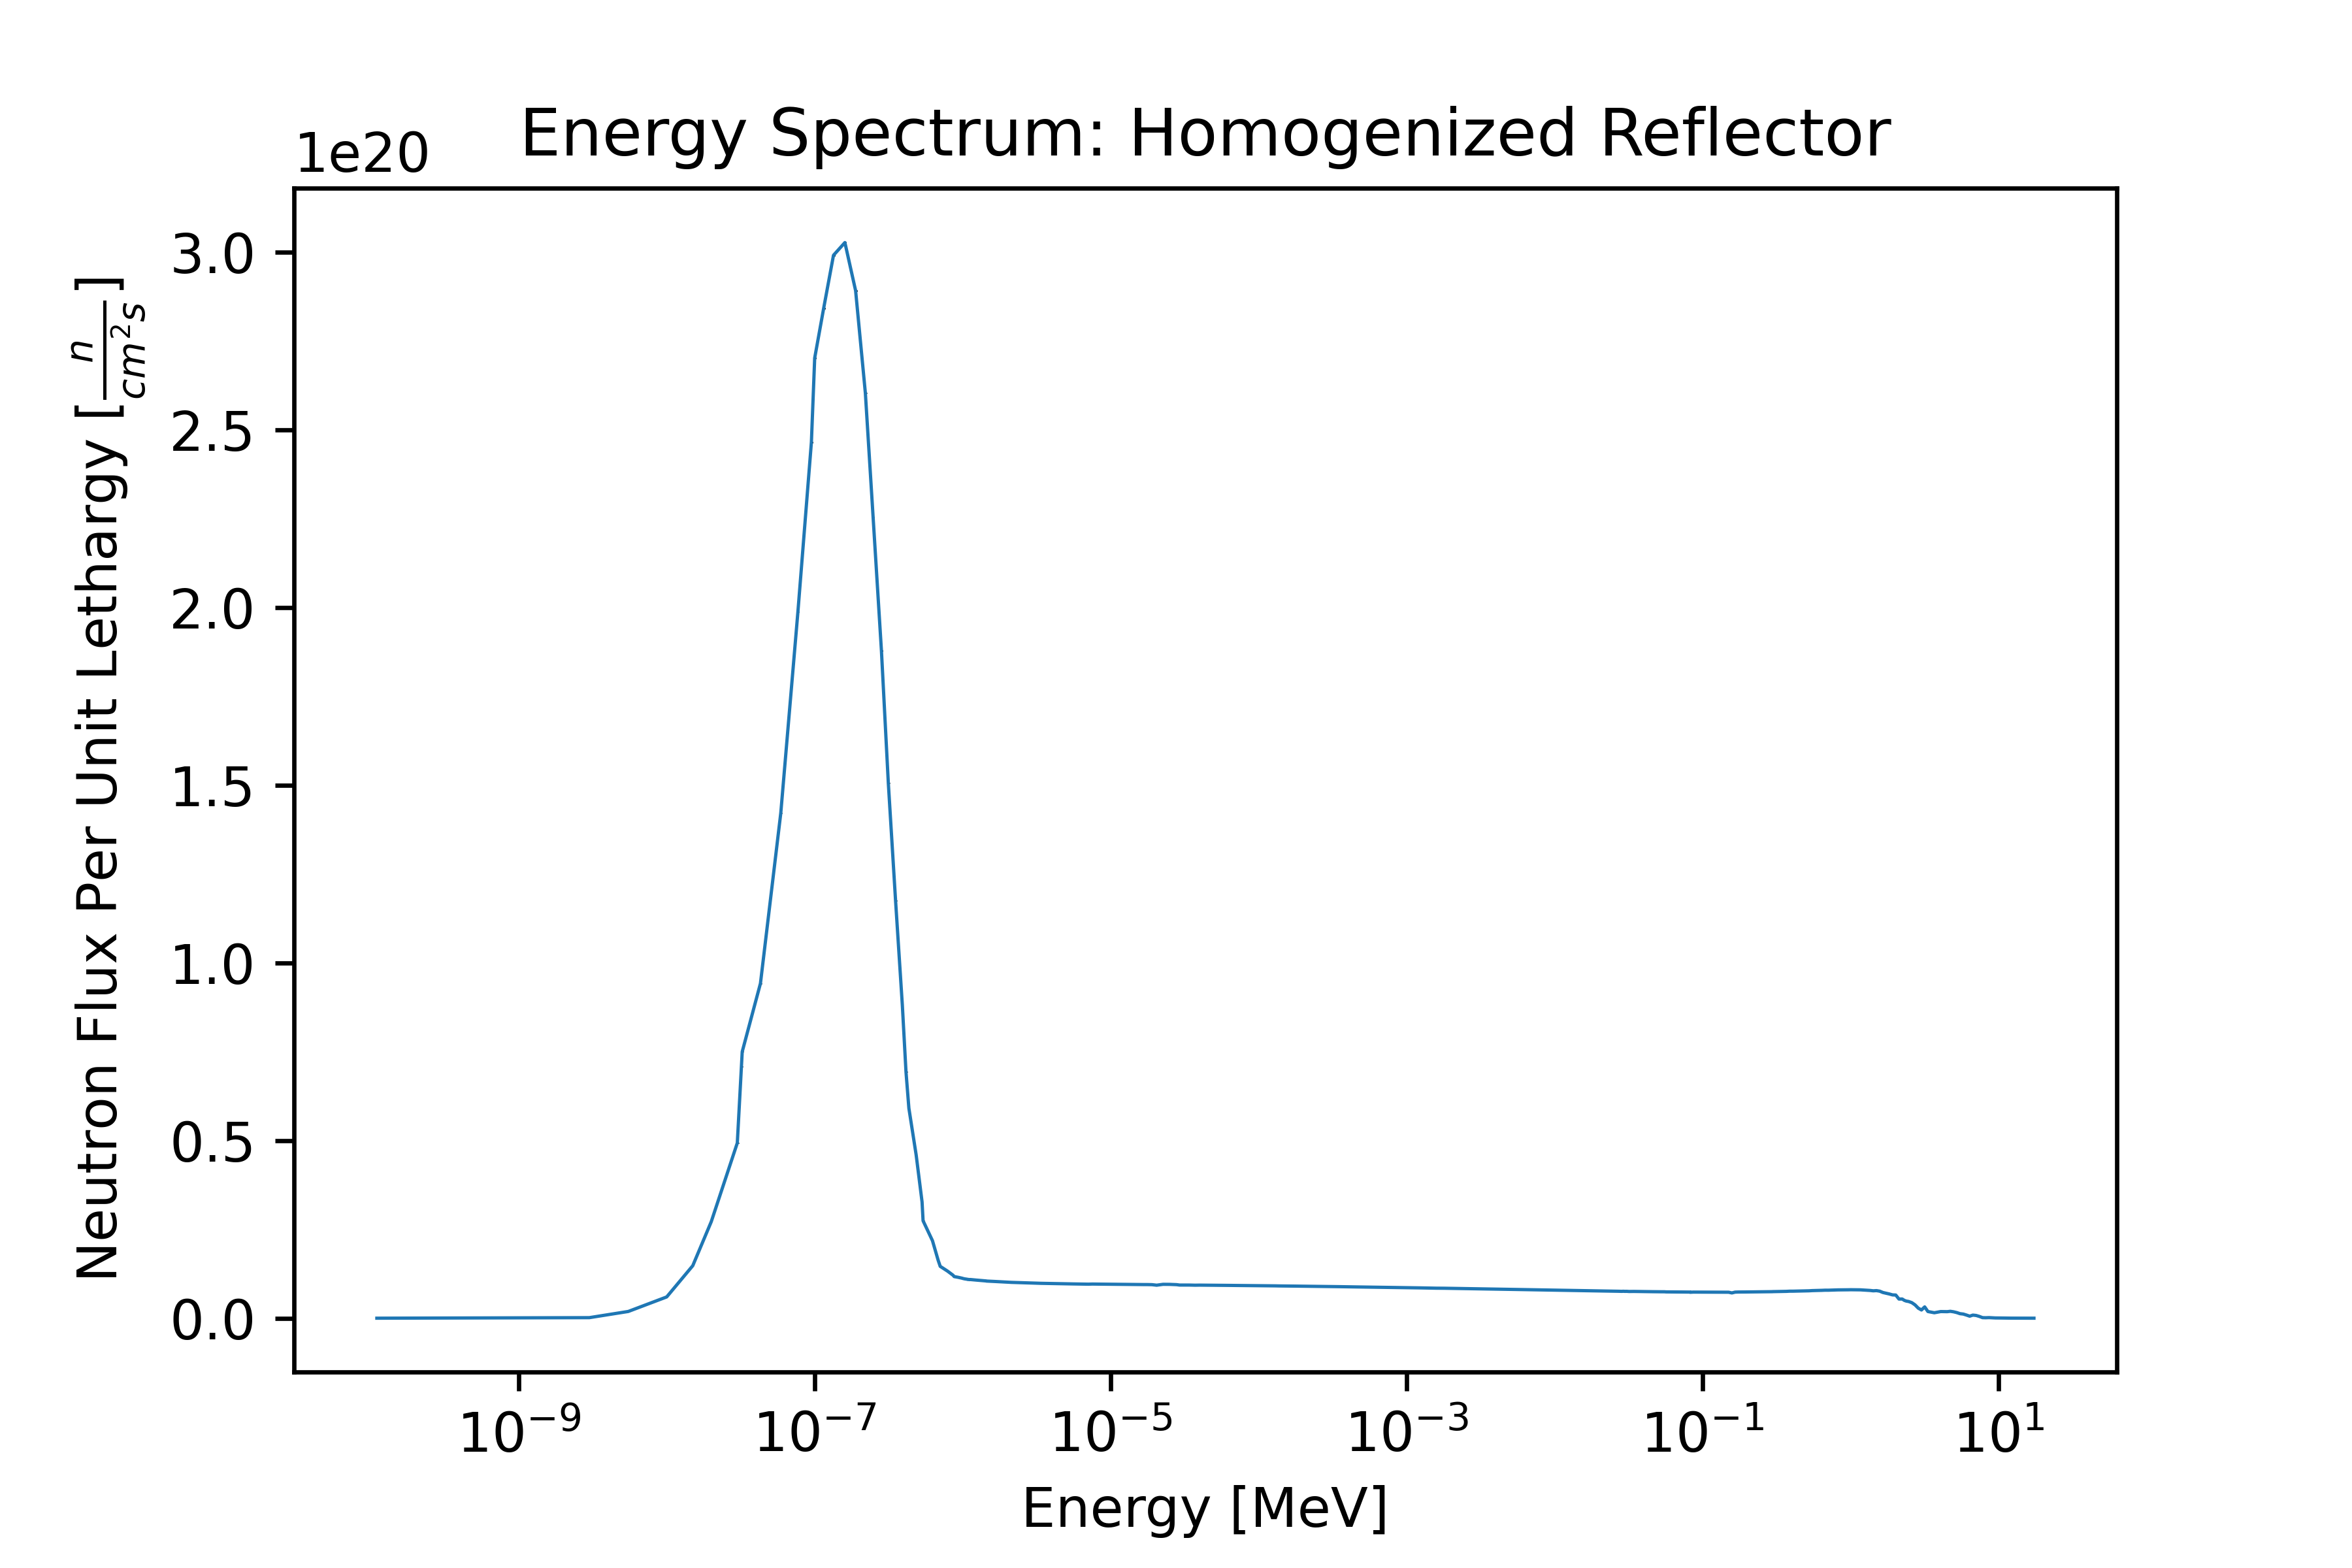
\includegraphics[width=0.95\linewidth]{figures/reflect_spec_homog}
  \caption{Reflector Spectrum}
  \label{fig:hom-reflec}
\end{subfigure}%
%

\caption{Lethargy Adjusted Neutron Flux Energy Spectra}
\label{fig:hom-spec}
\end{figure}

***these bad boys need to be bigger for sure  Also, while "homogenized pebbles" would be accurate, "homogenized coolant" and "homogenized reflector" make it sound like I did something to those materials, but I didn't.  I think at one point I used "Coolant of a Core Using Heterogenized Pebbles" but that's a bit long.***

Above, the energy spectra in the reflector, coolant, overall core, and a randomly selected fresh and 6th-pass pebble are provided.  The results are per unit lethargy and use the Tripoli 315-group energy structure.

The thermal peak of the whole-core and reflector both occur around 10E-07 MeV, which is also the energy of neutrons most-responsible for fission in this model.  The thermalization of neutrons in the reflector dominates the spectrum in \ref{fig:hom-core}, indicated by the high magnitude of the thermal peak in the reflector and core and their similar shape.

The spectra for a randomly selected fresh and 6 pass pebble are subject to the highest uncertainty of all the provided spectra in \ref{fig:hom-spec}, as a single pebble is a relatively small bin.  However, when coupled with the coolant spectra, \ref{fig:hom-cool}, they provide a clearer look at the flux energy spectrum in the active core region.  We can see that, while the thermal energy of the fresh and six-pass pebbles are similar in shape and magnitude, there is considerable difference in the higher energy range, due to the buildup of fission products and the decrease in U-235 concentration.


\section{Effect of Homogenizing}

The results above all use the assumption of a pebble that has the TRISO particles homogenized and blended with the rest of the pebble matrix in the region containing fuel.  However, as reported in \cite{brown_stochastic_2005}, homogenization can cause under-predictions of k-eff as large as 5-6\%.  And so, an otherwise identical model with explicitly modeled TRISO particles (the fuel kernel and all four protective layers are explicitly modeled) is used to investigate the effect of homogenization.  As a reminder, the isotopic compositions are pulled from a burnup simulation using an infinite lattice of pebbles with explicitly modeled TRISOs.  As such, the isotopic compositions between the homogenized and heterogenized models are identical.


\begin{figure}[H]
\centering

\begin{subfigure}{0.45\textwidth}
  \includegraphics[width=0.95\linewidth]{figures/het/het-r}
  \caption{Radial Cross Section at y=0}
  \label{fig:heta}
\end{subfigure}%
%
\begin{subfigure}{0.45\textwidth}
  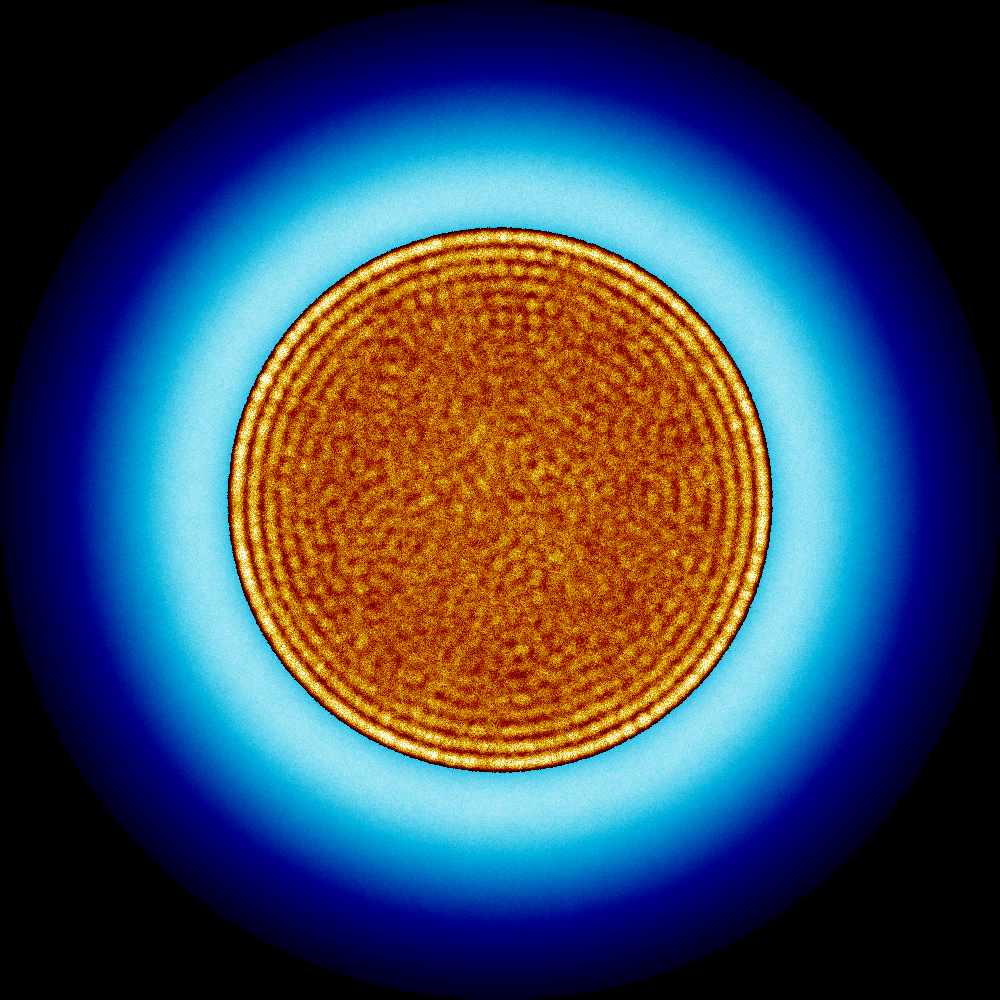
\includegraphics[width=0.95\linewidth]{figures/het/het-rm}
  \caption{Radial Mesh}
  \label{fig:hetb}
\end{subfigure}

\begin{subfigure}{0.45\textwidth}
  \includegraphics[width=0.95\linewidth]{figures/het/het-v}
  \caption{Axial Cross Section at z=0 }
  \label{fig:hetc}
\end{subfigure}
%
\begin{subfigure}{0.45\textwidth}
  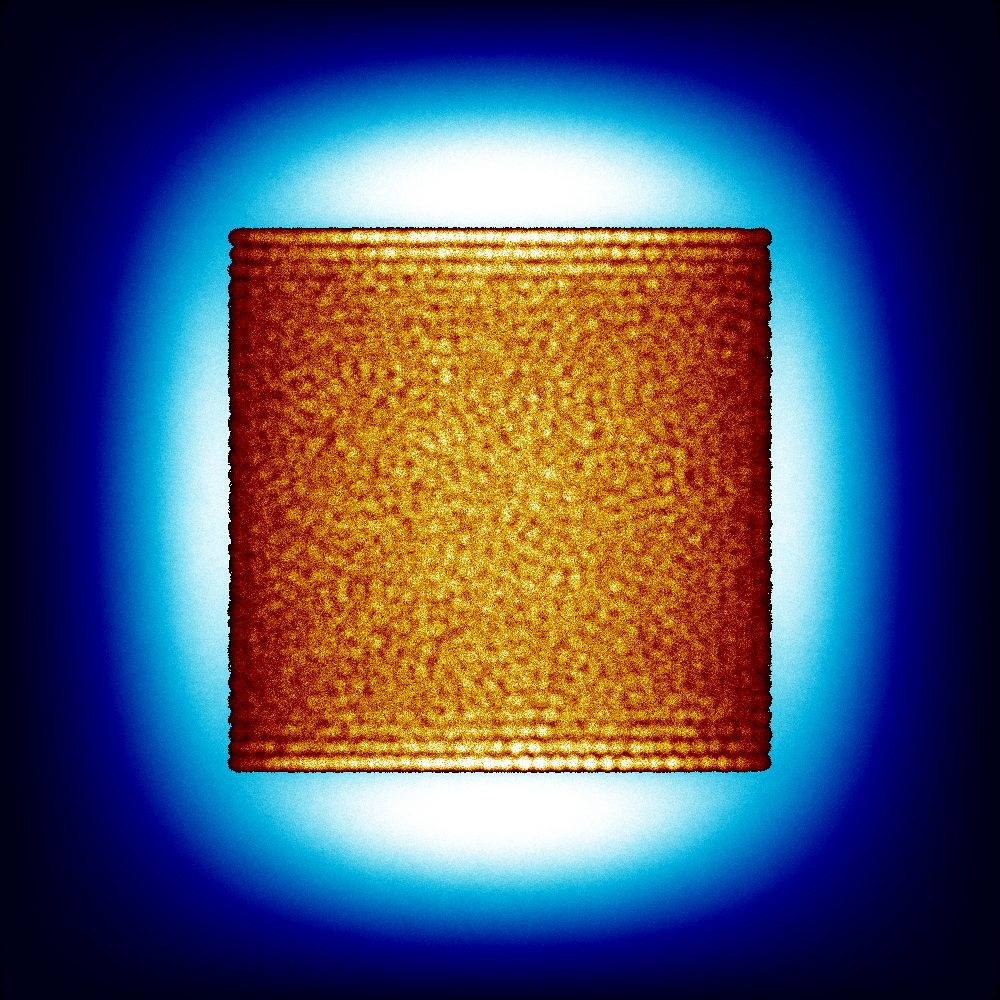
\includegraphics[width=0.95\linewidth]{figures/het/het-vm}
  \caption{Axial Mesh}
  \label{fig:hetd}
\end{subfigure}
%
\caption{Full Core Using Heterogenized Pebbles}
\label{fig:het}
\end{figure}


In agreement with \cite{brown_stochastic_2005}, the heterogenized model reported a k-eff of 1.087 +/- 0.00032, compared to the homogenized model's 1.041 +/- 0.00054, a difference of 4.23\%.  

Overall, the mesh result for the fission rate is much the same - the banding patterns are still present, if slightly less defined.  While \ref{fig:het} best serves as a qualitative visualization aid, figures \ref{fig:het-det-xy}, \ref{fig:het-det-z}, and \ref{fig:het-det-plane} support this in a more quantitative manner.


\begin{figure}[H]
\centering

\begin{subfigure}{0.9\textwidth}
  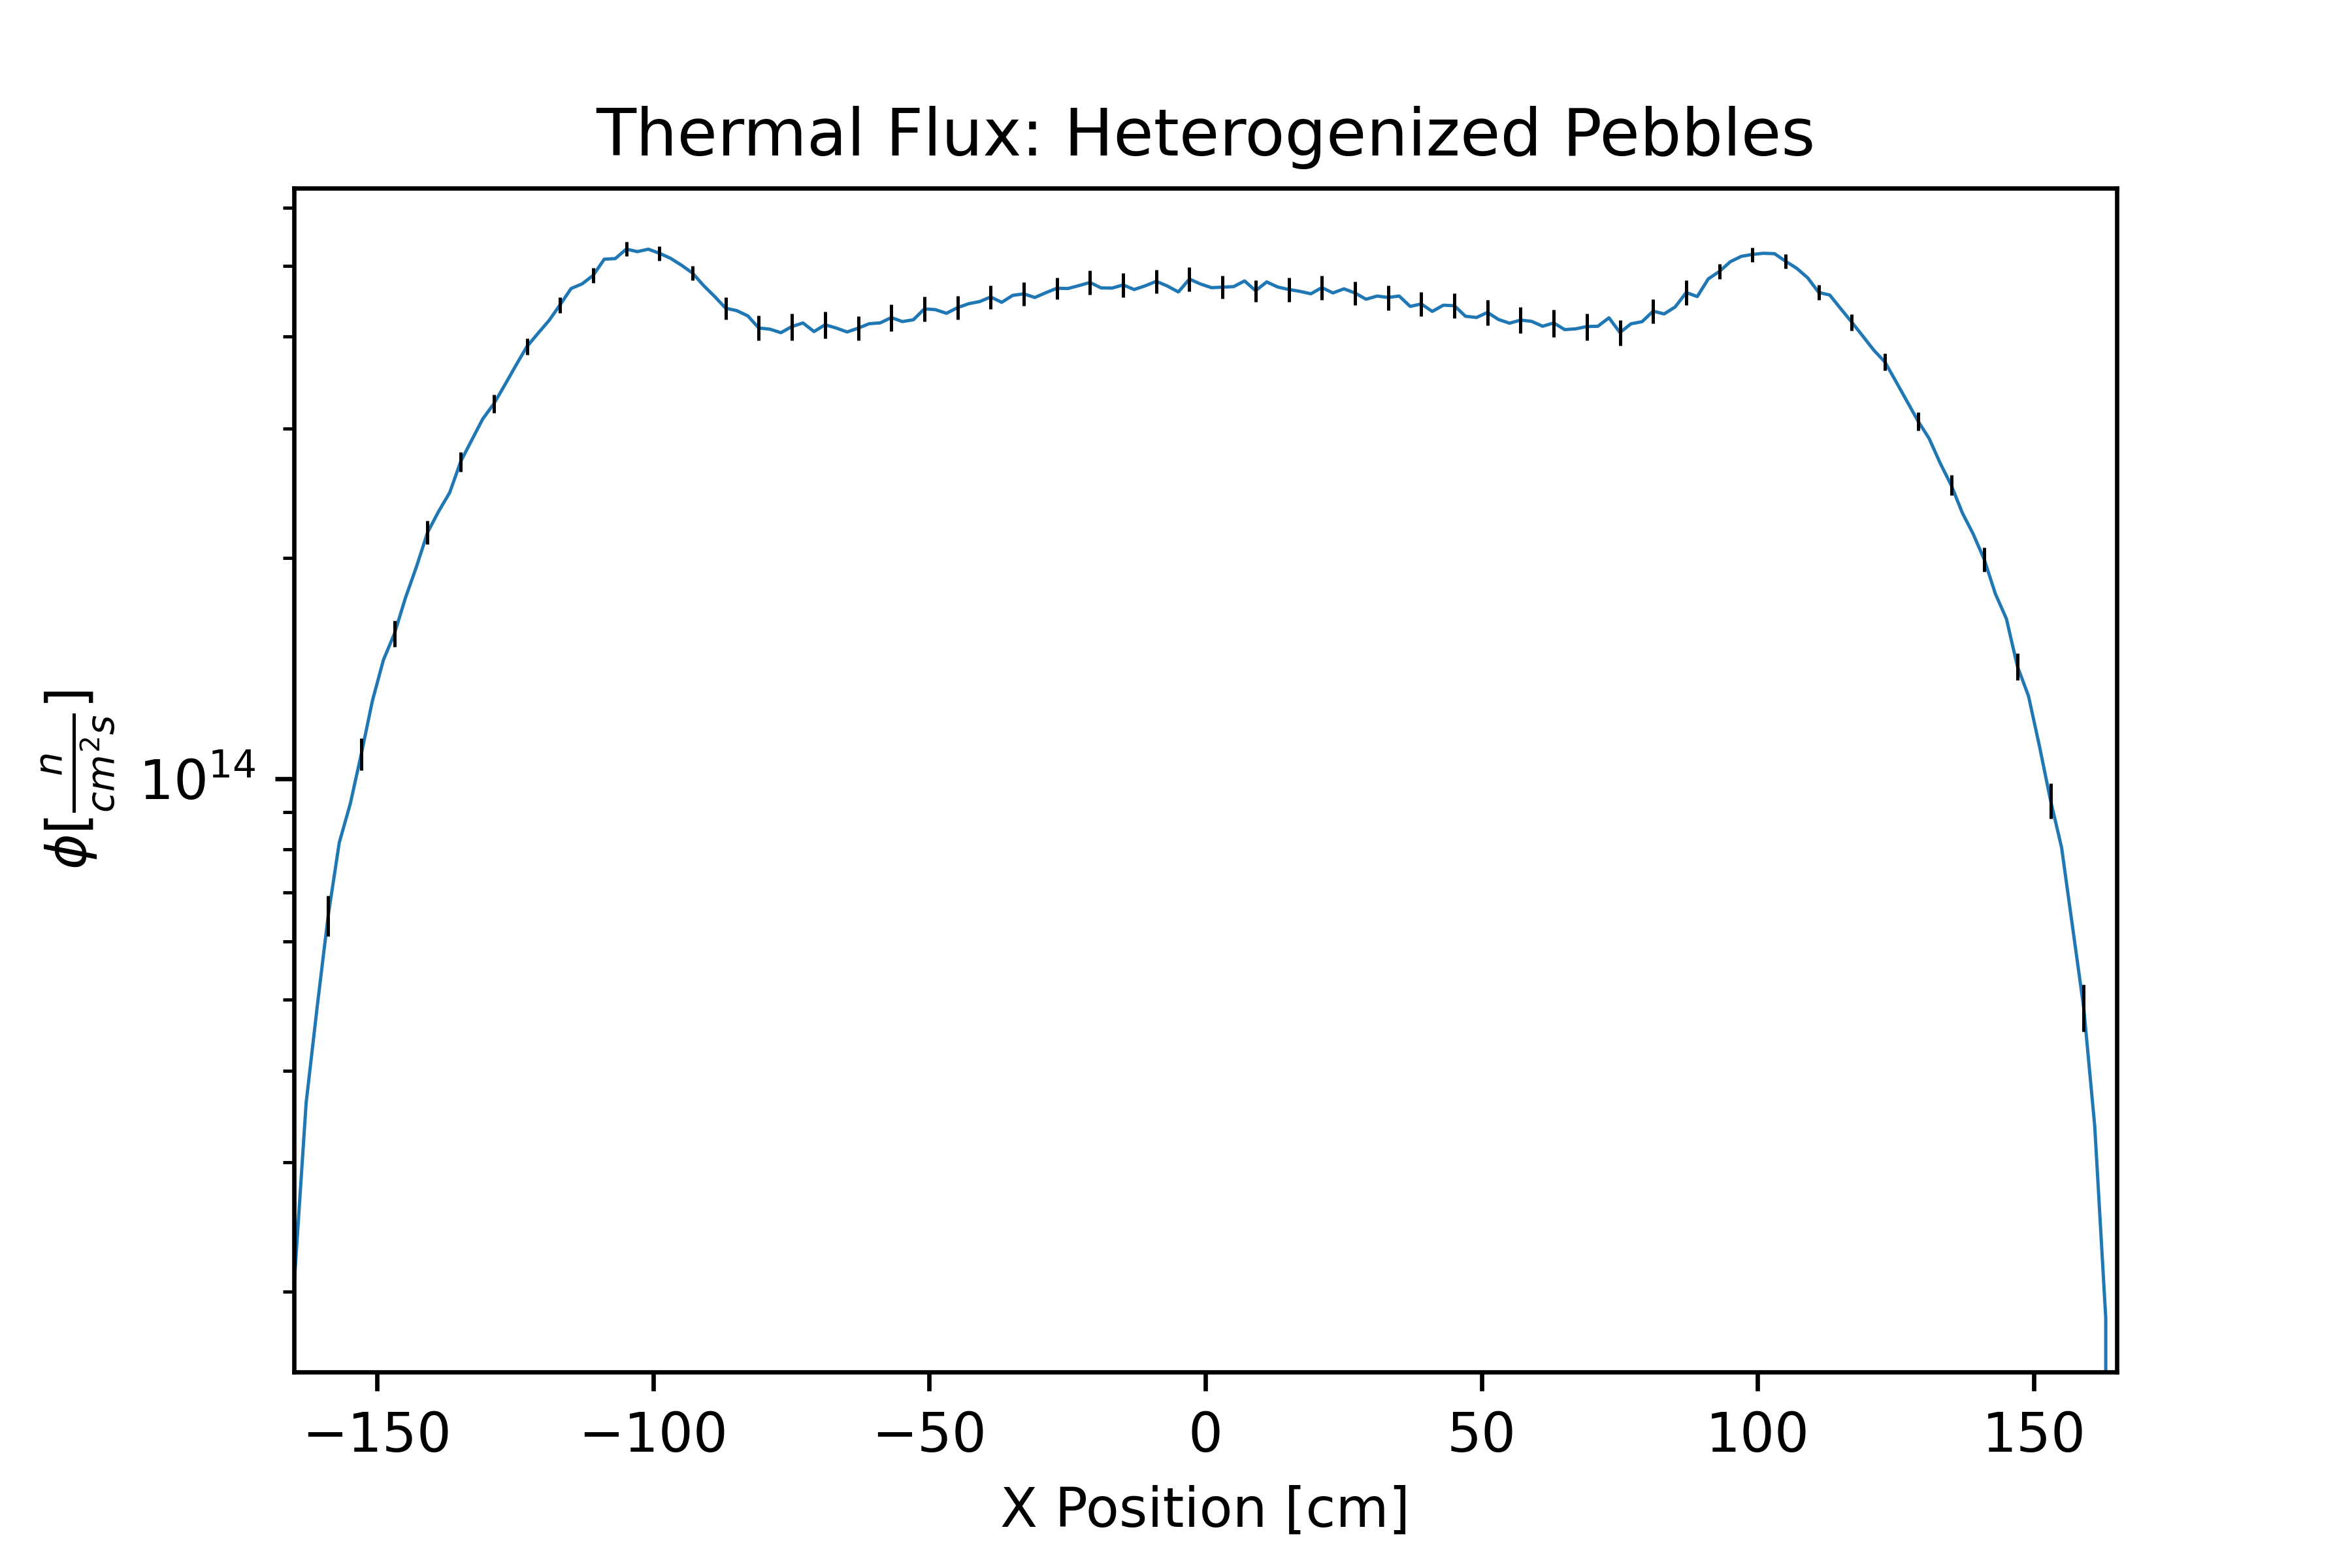
\includegraphics[width=0.95\linewidth]{figures/therm_flux_het.png}
  \caption{Thermal Flux}
  \label{fig:het-det-xy-therm}
\end{subfigure}%

\caption{Radial Thermal and Fast Flux Profiles: Heterogenized Pebbles}
\end{figure}

\begin{figure}[H]\ContinuedFloat
\centering

\begin{subfigure}{0.9\textwidth}
  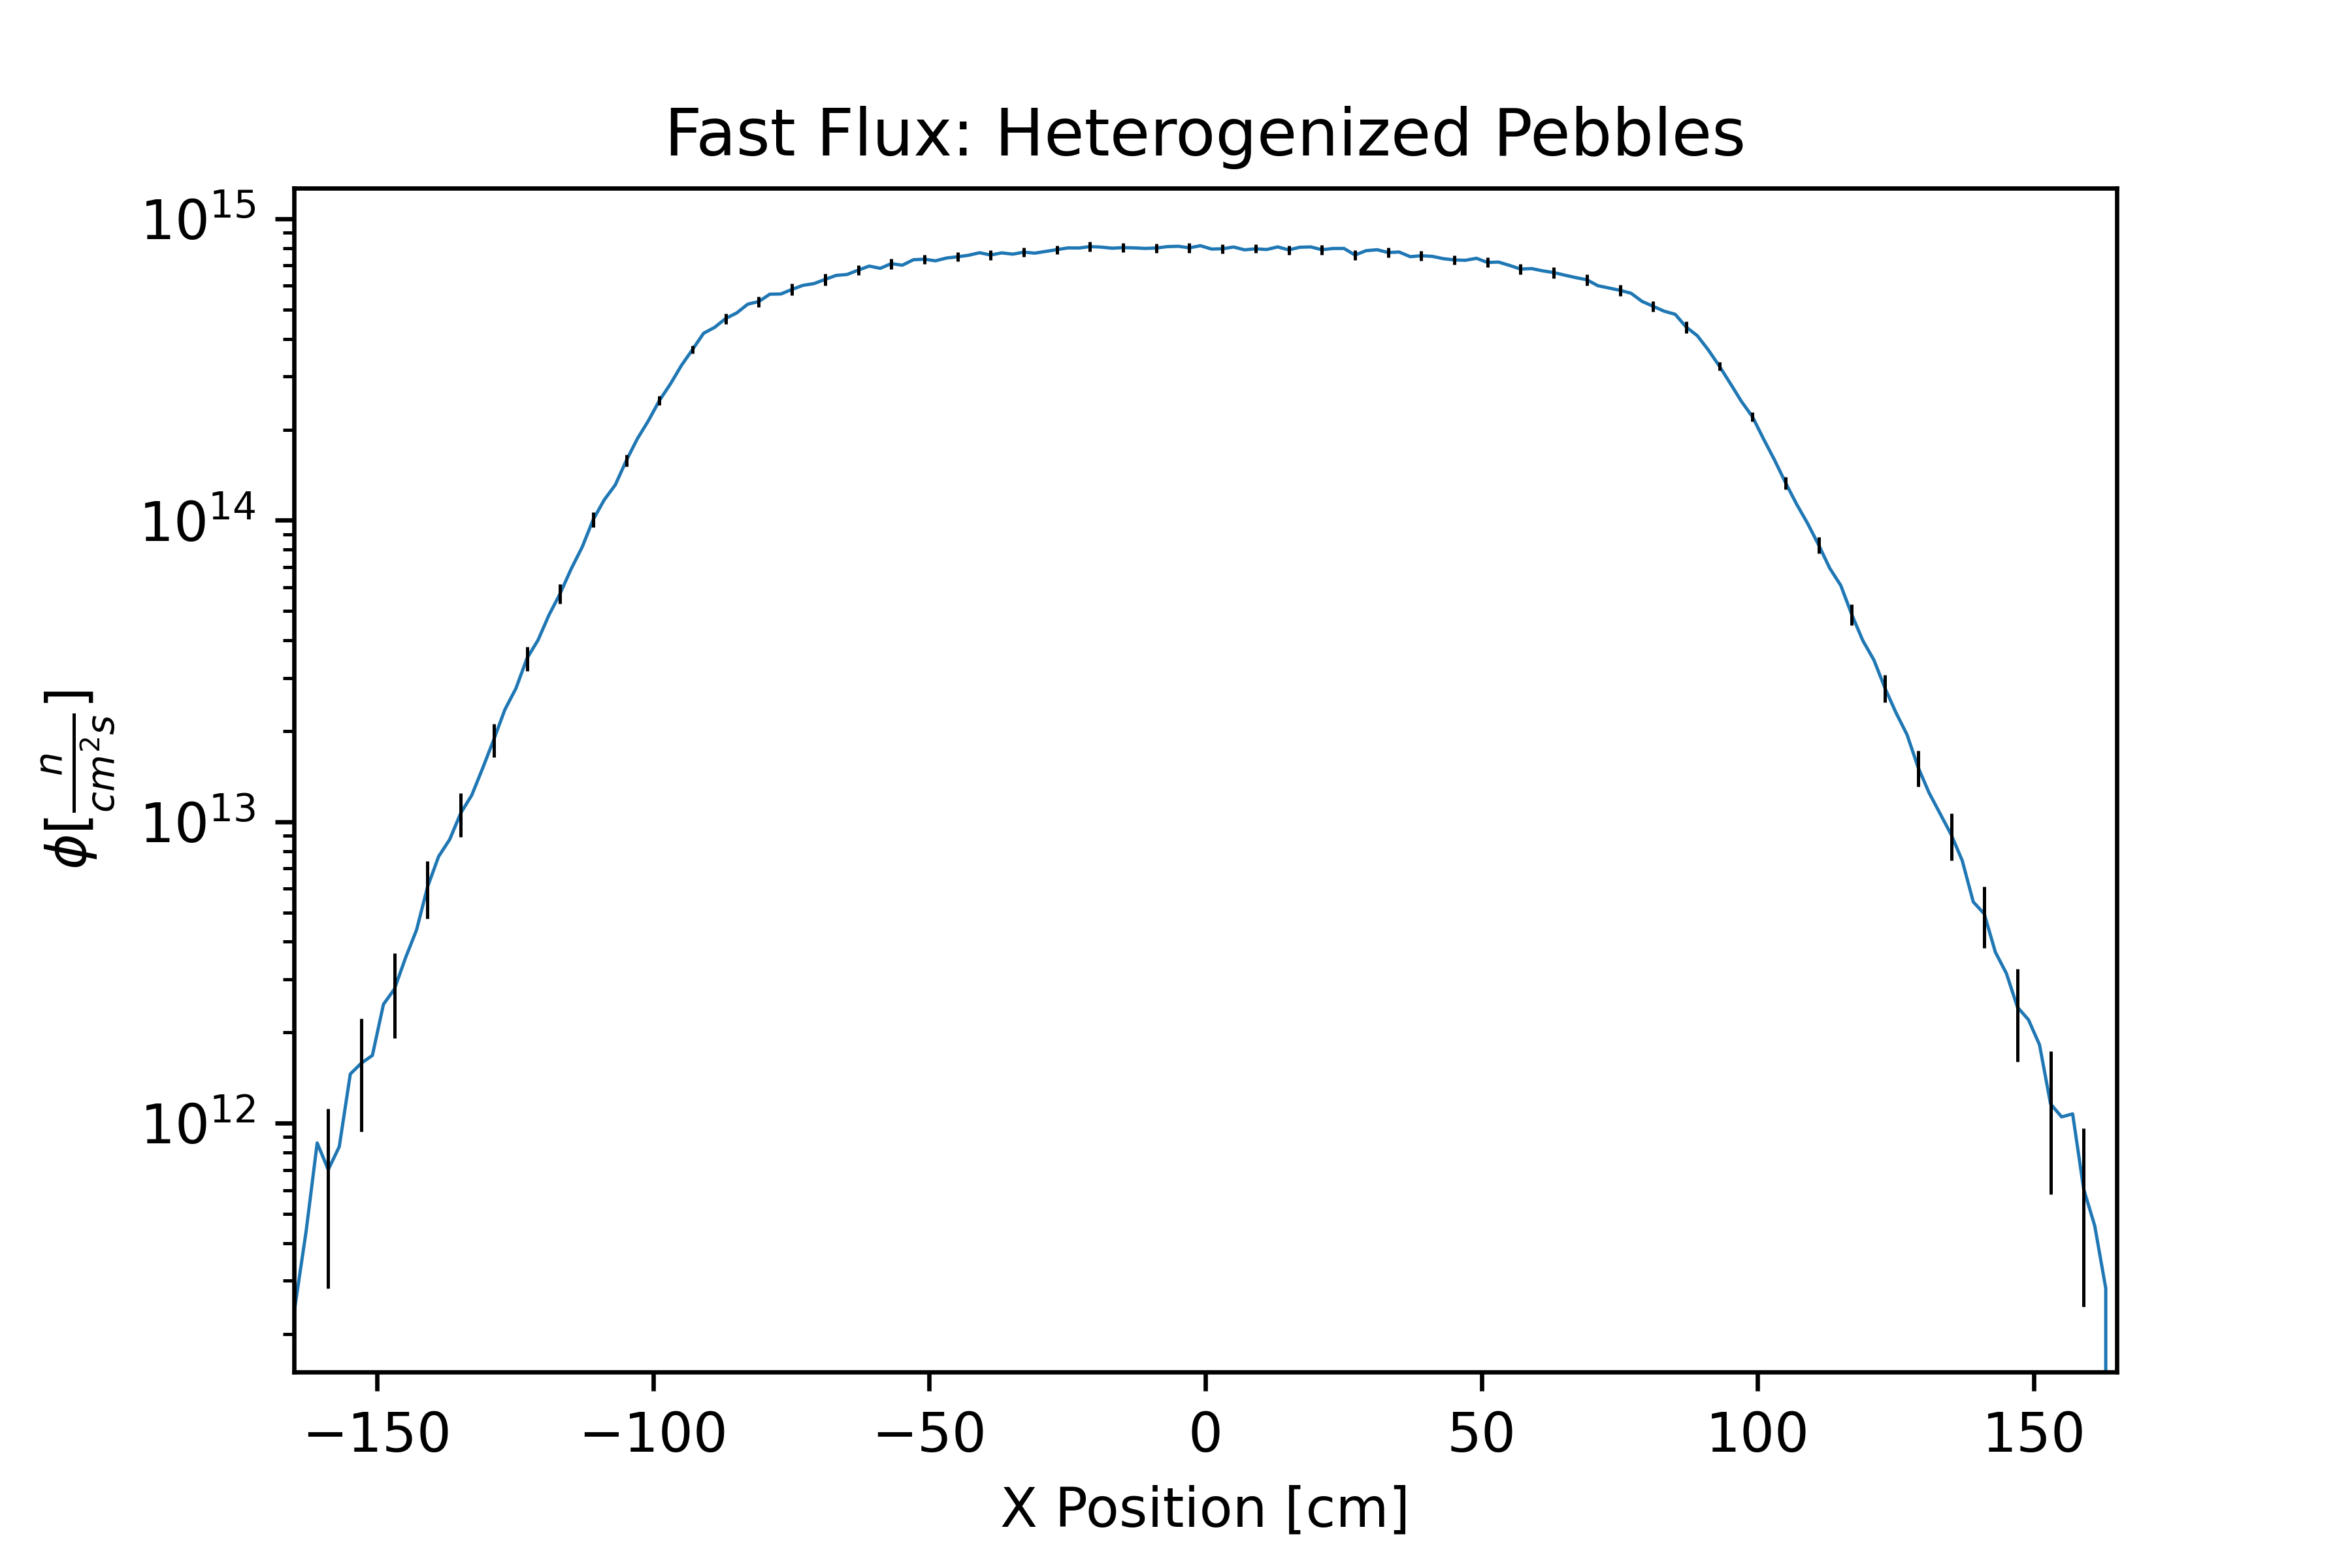
\includegraphics[width=0.95\linewidth]{figures/fast_flux_het.png}
  \caption{Fast Flux}
  \label{fig:het-det-xy-fast}
\end{subfigure}


\caption{Radial Thermal and Fast Flux Profiles: Heterogenized Pebbles (cont.)}
\label{fig:het-det-xy}
\end{figure}


Compared to the homogenized model, the heterogenized Sangamon20 core reports a slightly lower neutron current at the outer edge of the reflector, at 5.718E+11 +/- 1.735E-09, an absolute difference of approximately 2.0E+09.  The heterogenized model otherwise shows a similar flux profile to the homogenized model, and experiences a similar level of uncertainty in the outer edges of the reflector for the fast flux profiles, likely due to the significant thermalization of neutrons by that point in the reflector.


\begin{figure}[H]
\centering

  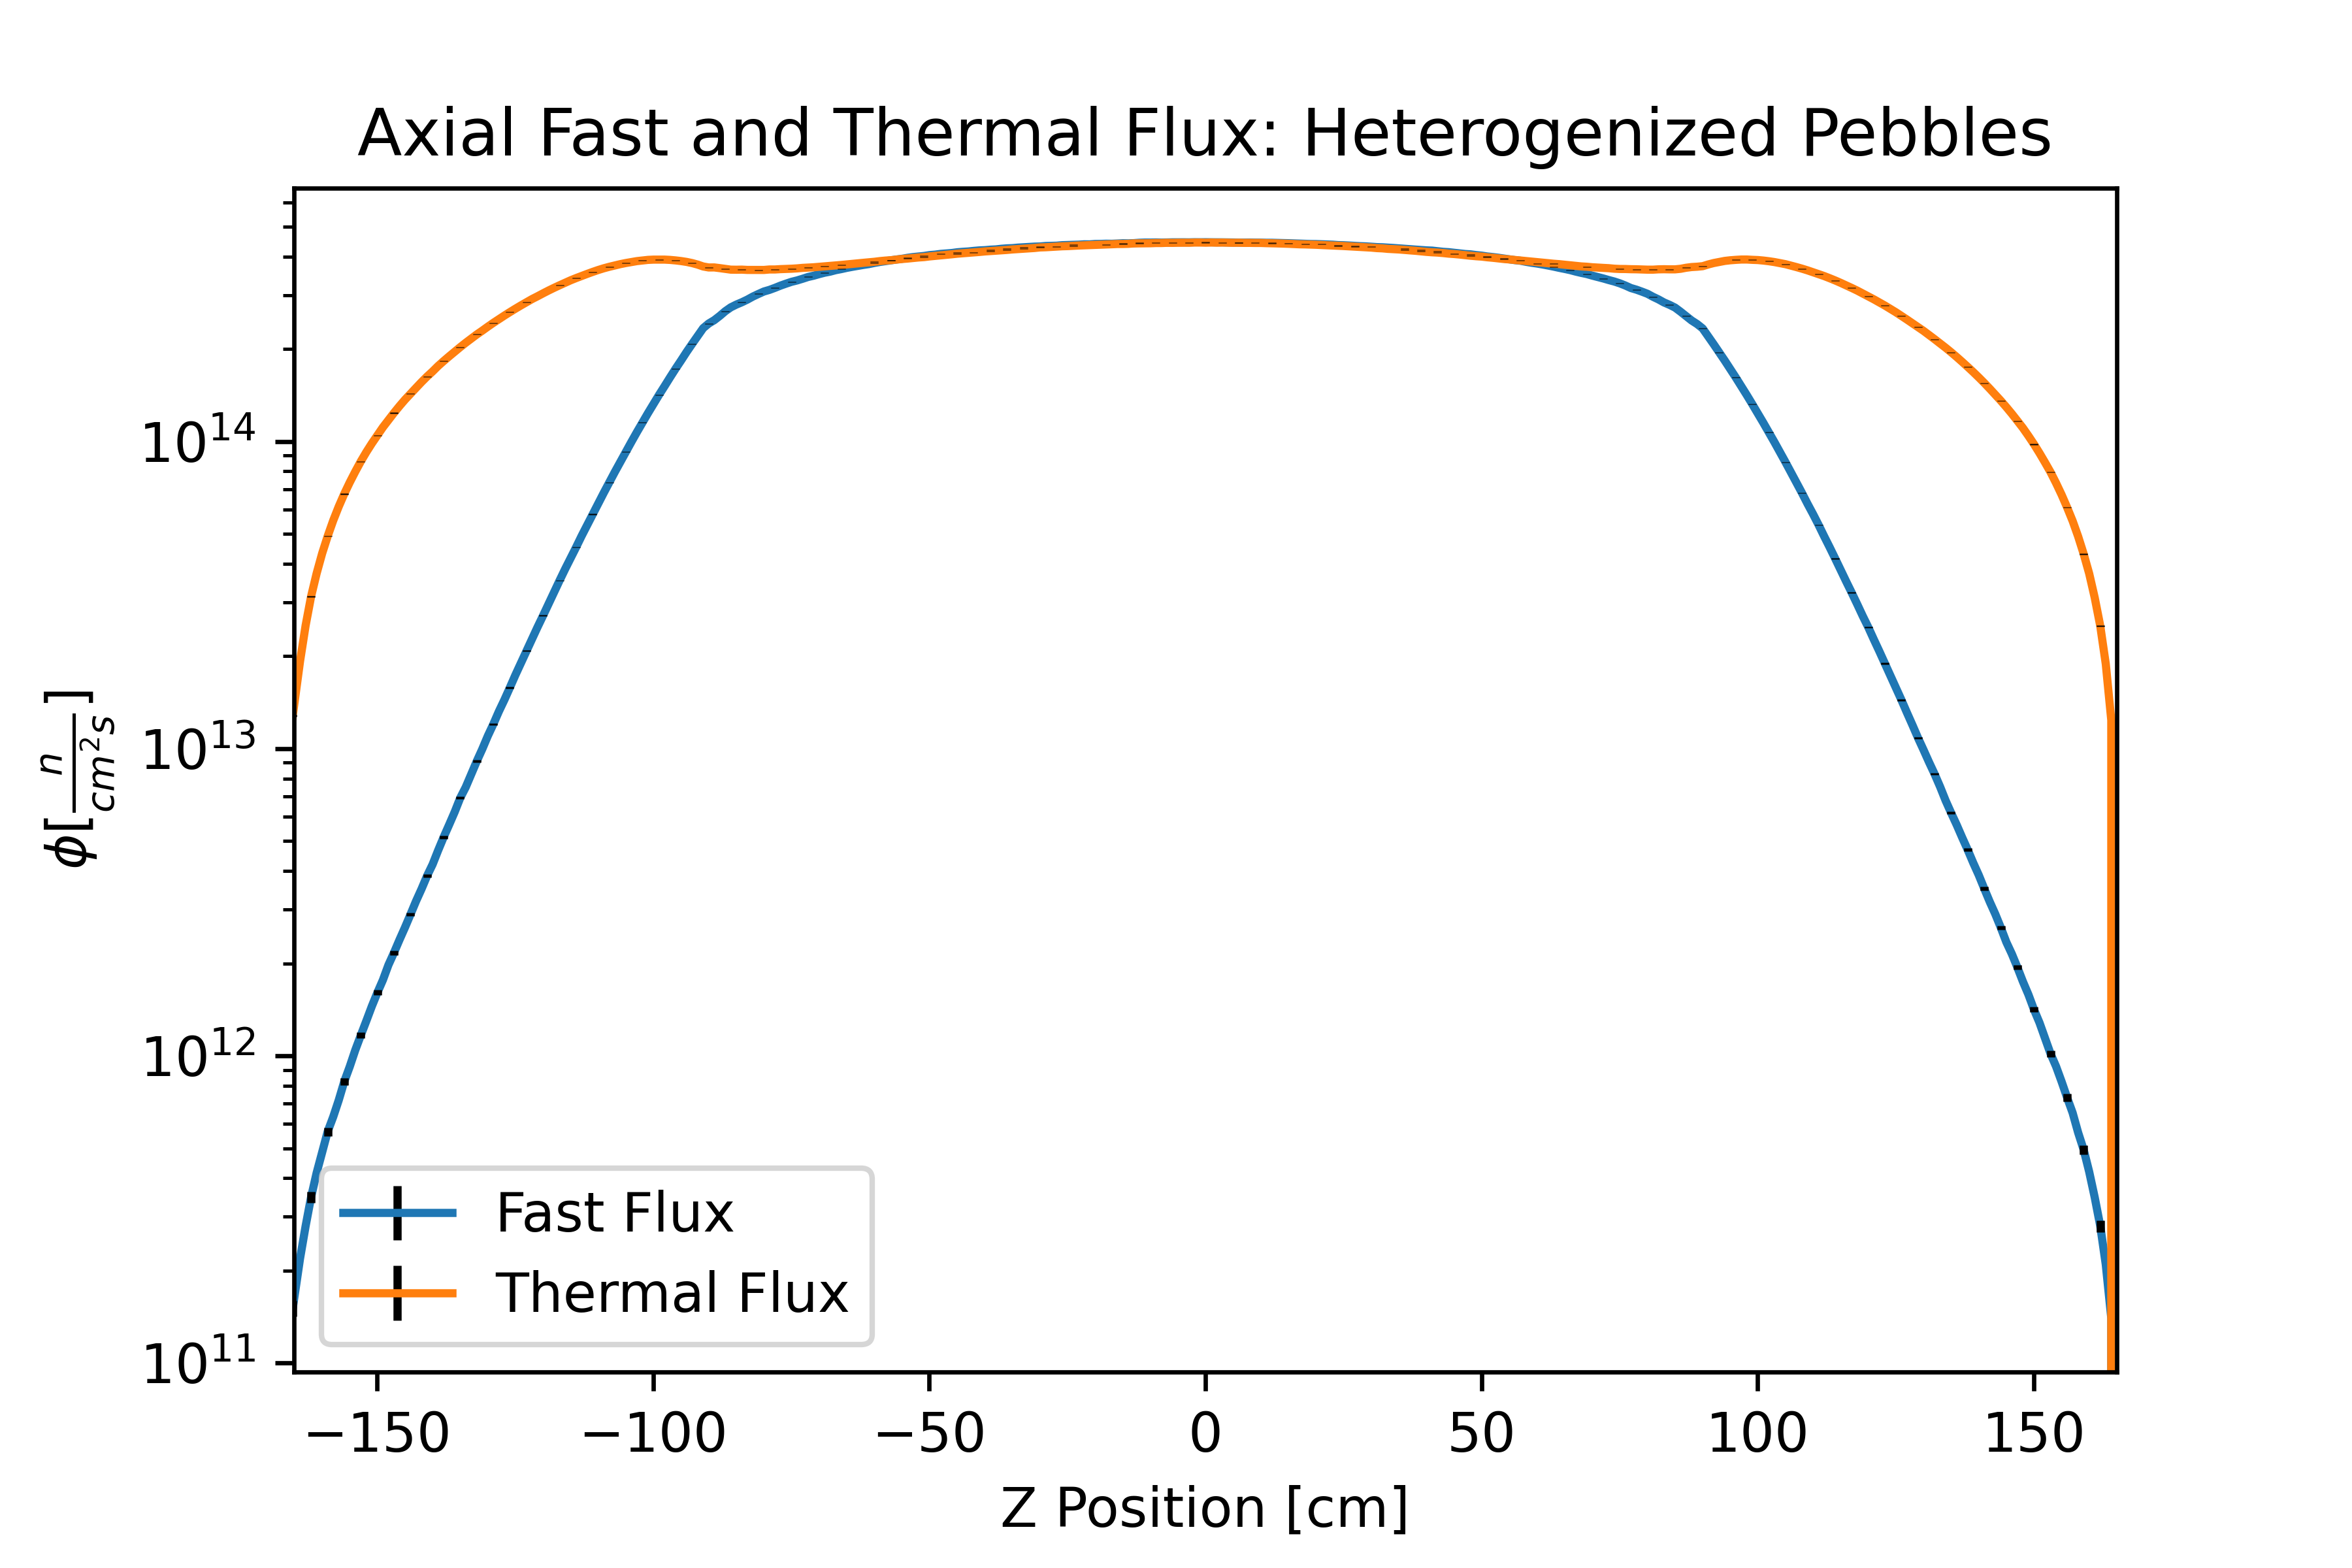
\includegraphics[width=0.95\linewidth]{figures/fast_therm_flux_het_z.png}

\caption{Axial Thermal and Fast Flux Profiles along the Centerline in Sangamon20: Heterogenized Pebbles}
\label{fig:het-det-z}
\end{figure}


\begin{figure}[H]
\centering


\includegraphics[width=0.95\linewidth]{figures/therm_xy_plane_het_er.png}
\caption{Thermal Flux in xy Plane in Sangamon20: Heterogenized Pebbles.  The dotted line annotation marks the boundary between the active core and the graphite reflector.}
\label{fig:het-plane-therm}

\end{figure}

\begin{figure}[H]
\centering

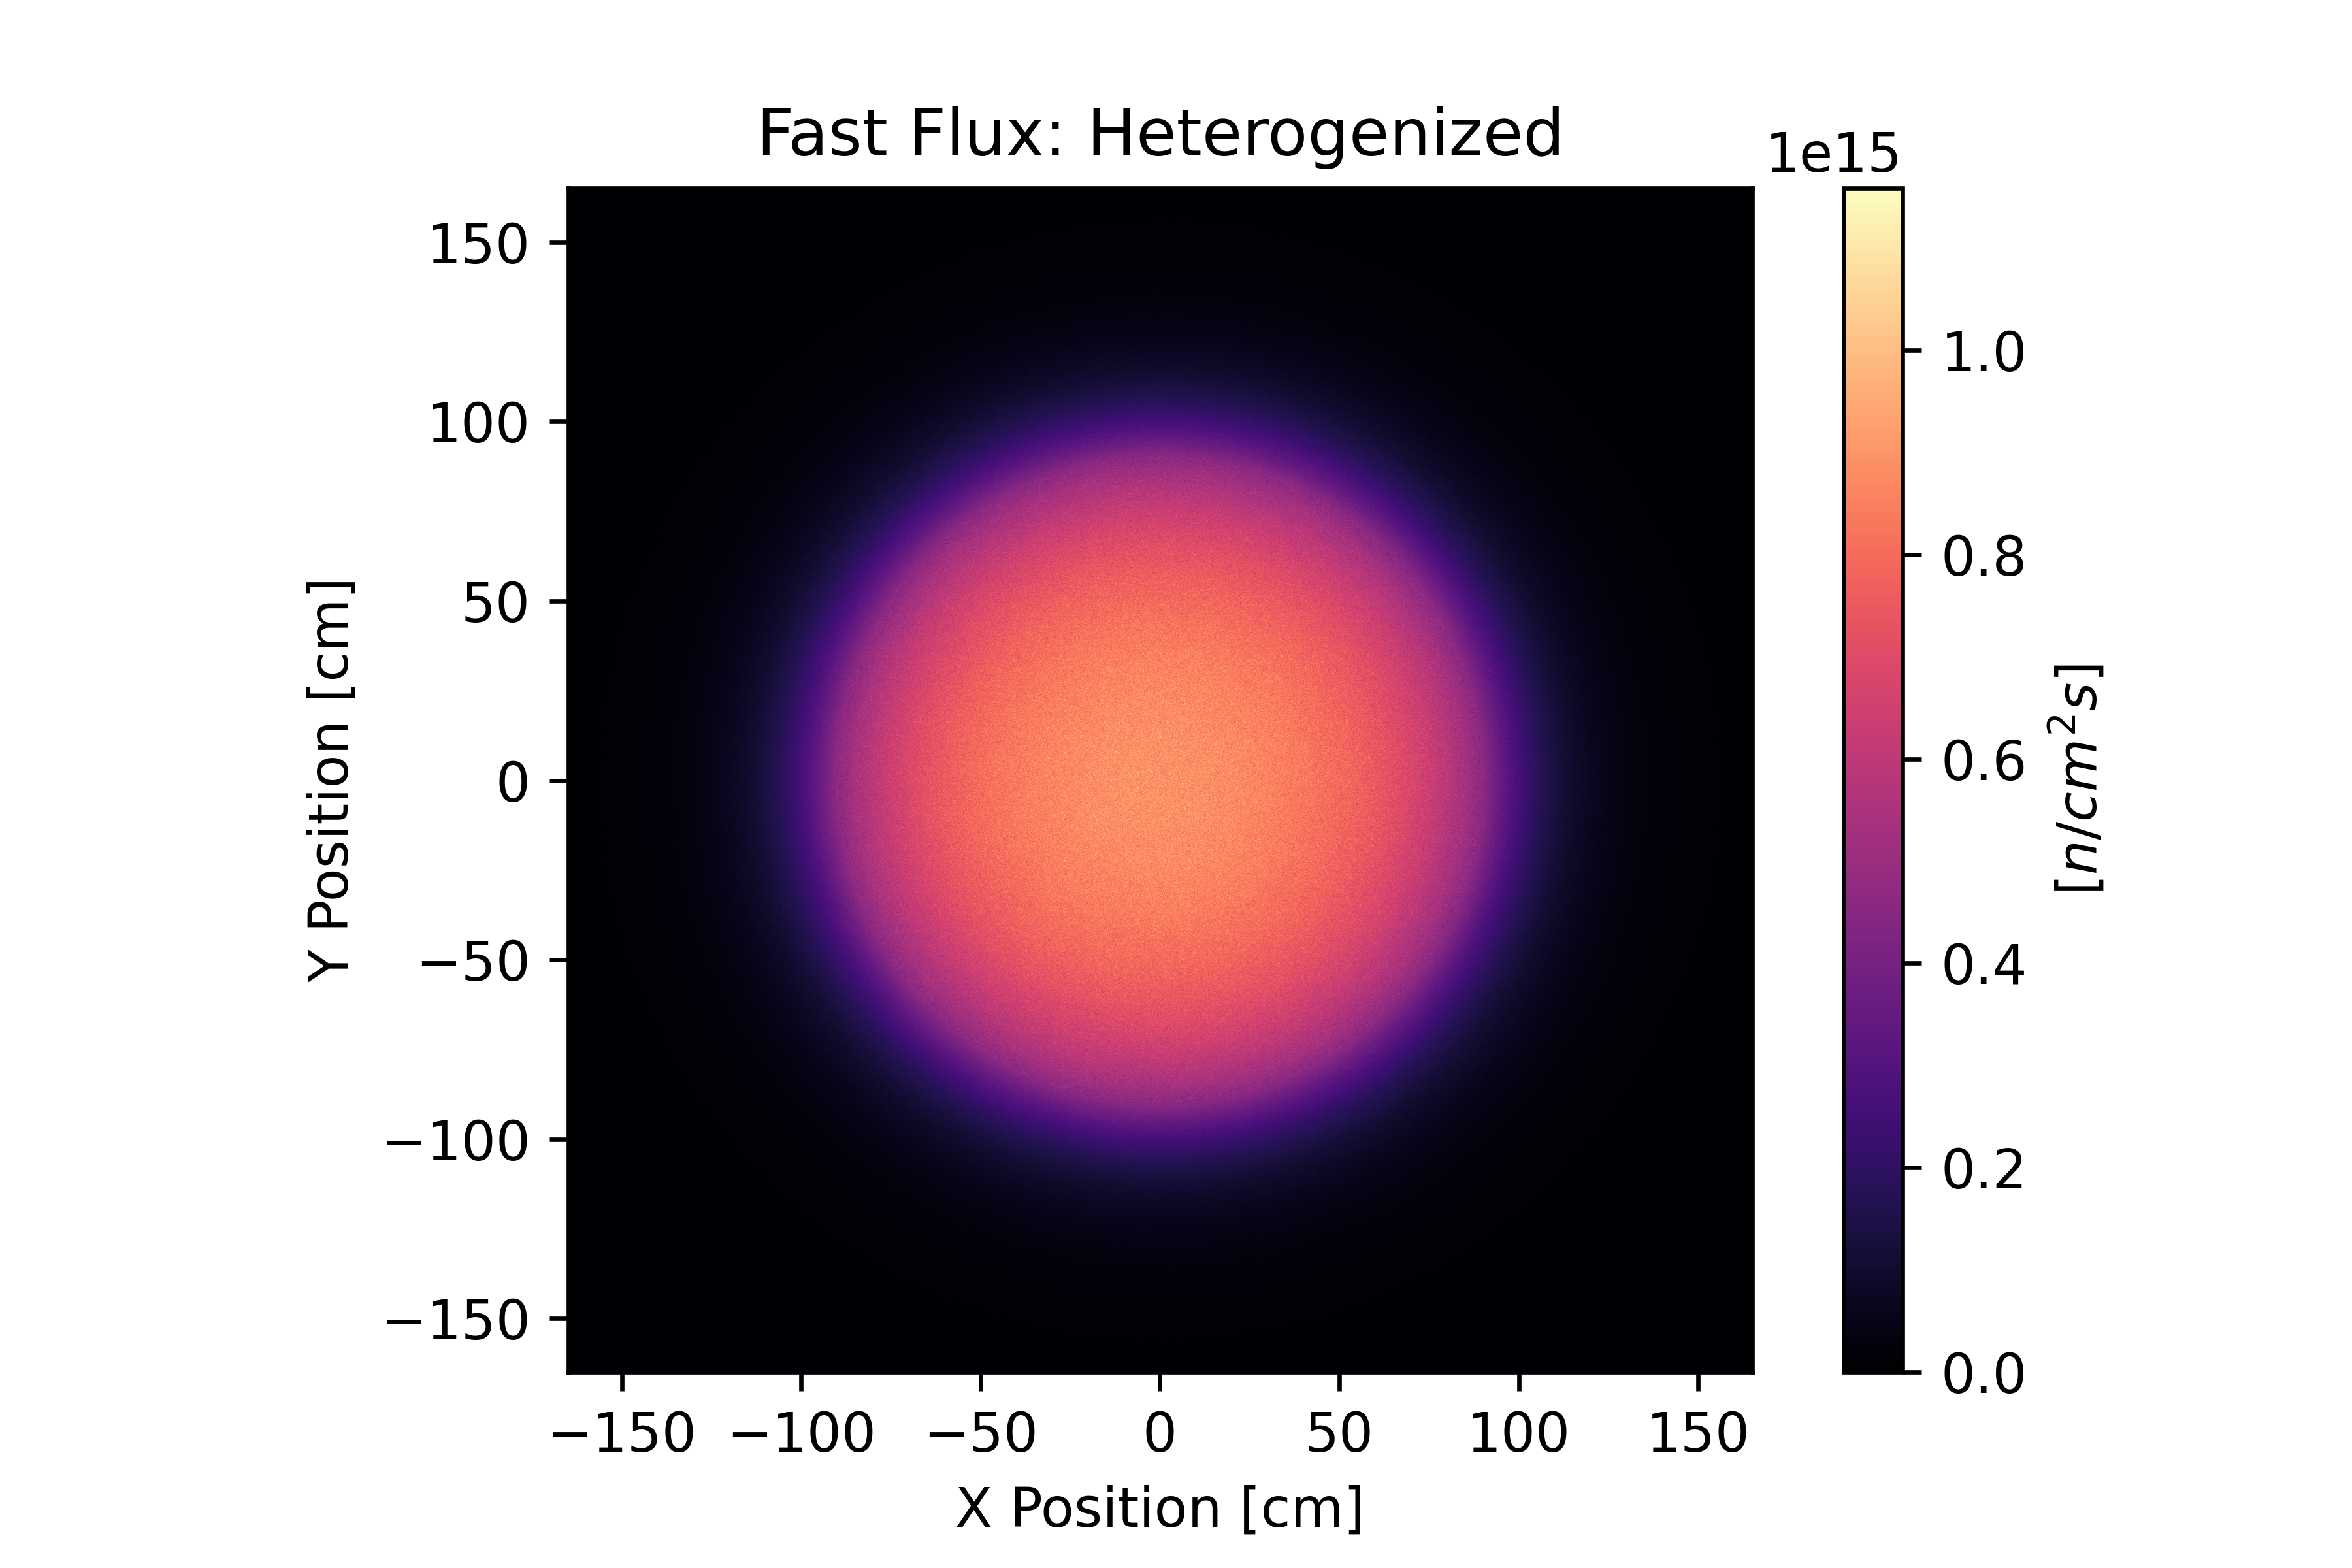
\includegraphics[width=0.95\linewidth]{figures/fast_xy_plane_het_er.png}
\caption{Fast Flux in xy Plane in Sangamon20: Heterogenized Pebbles.  The dotted line annotation marks the boundary between the active core and the graphite reflector.}
\label{fig:het-plane-fast}

\end{figure}

Compared to Figure *** ref homo xy plane mesh **, the edge pebble bands are much less distinct.  This is because the homogenized pebbles have the fissile material spread over the entirety of the 2.5 cm radius fueled center.  The heterogenized pebbles, meanwhile, may have the same number of fissile atoms, but the regions capable of fission are concentrated to the TRISO kernel.  The rest of the pebble consists of its graphite matrix.


\begin{figure}[H]
\centering

\begin{subfigure}{0.95\textwidth}
  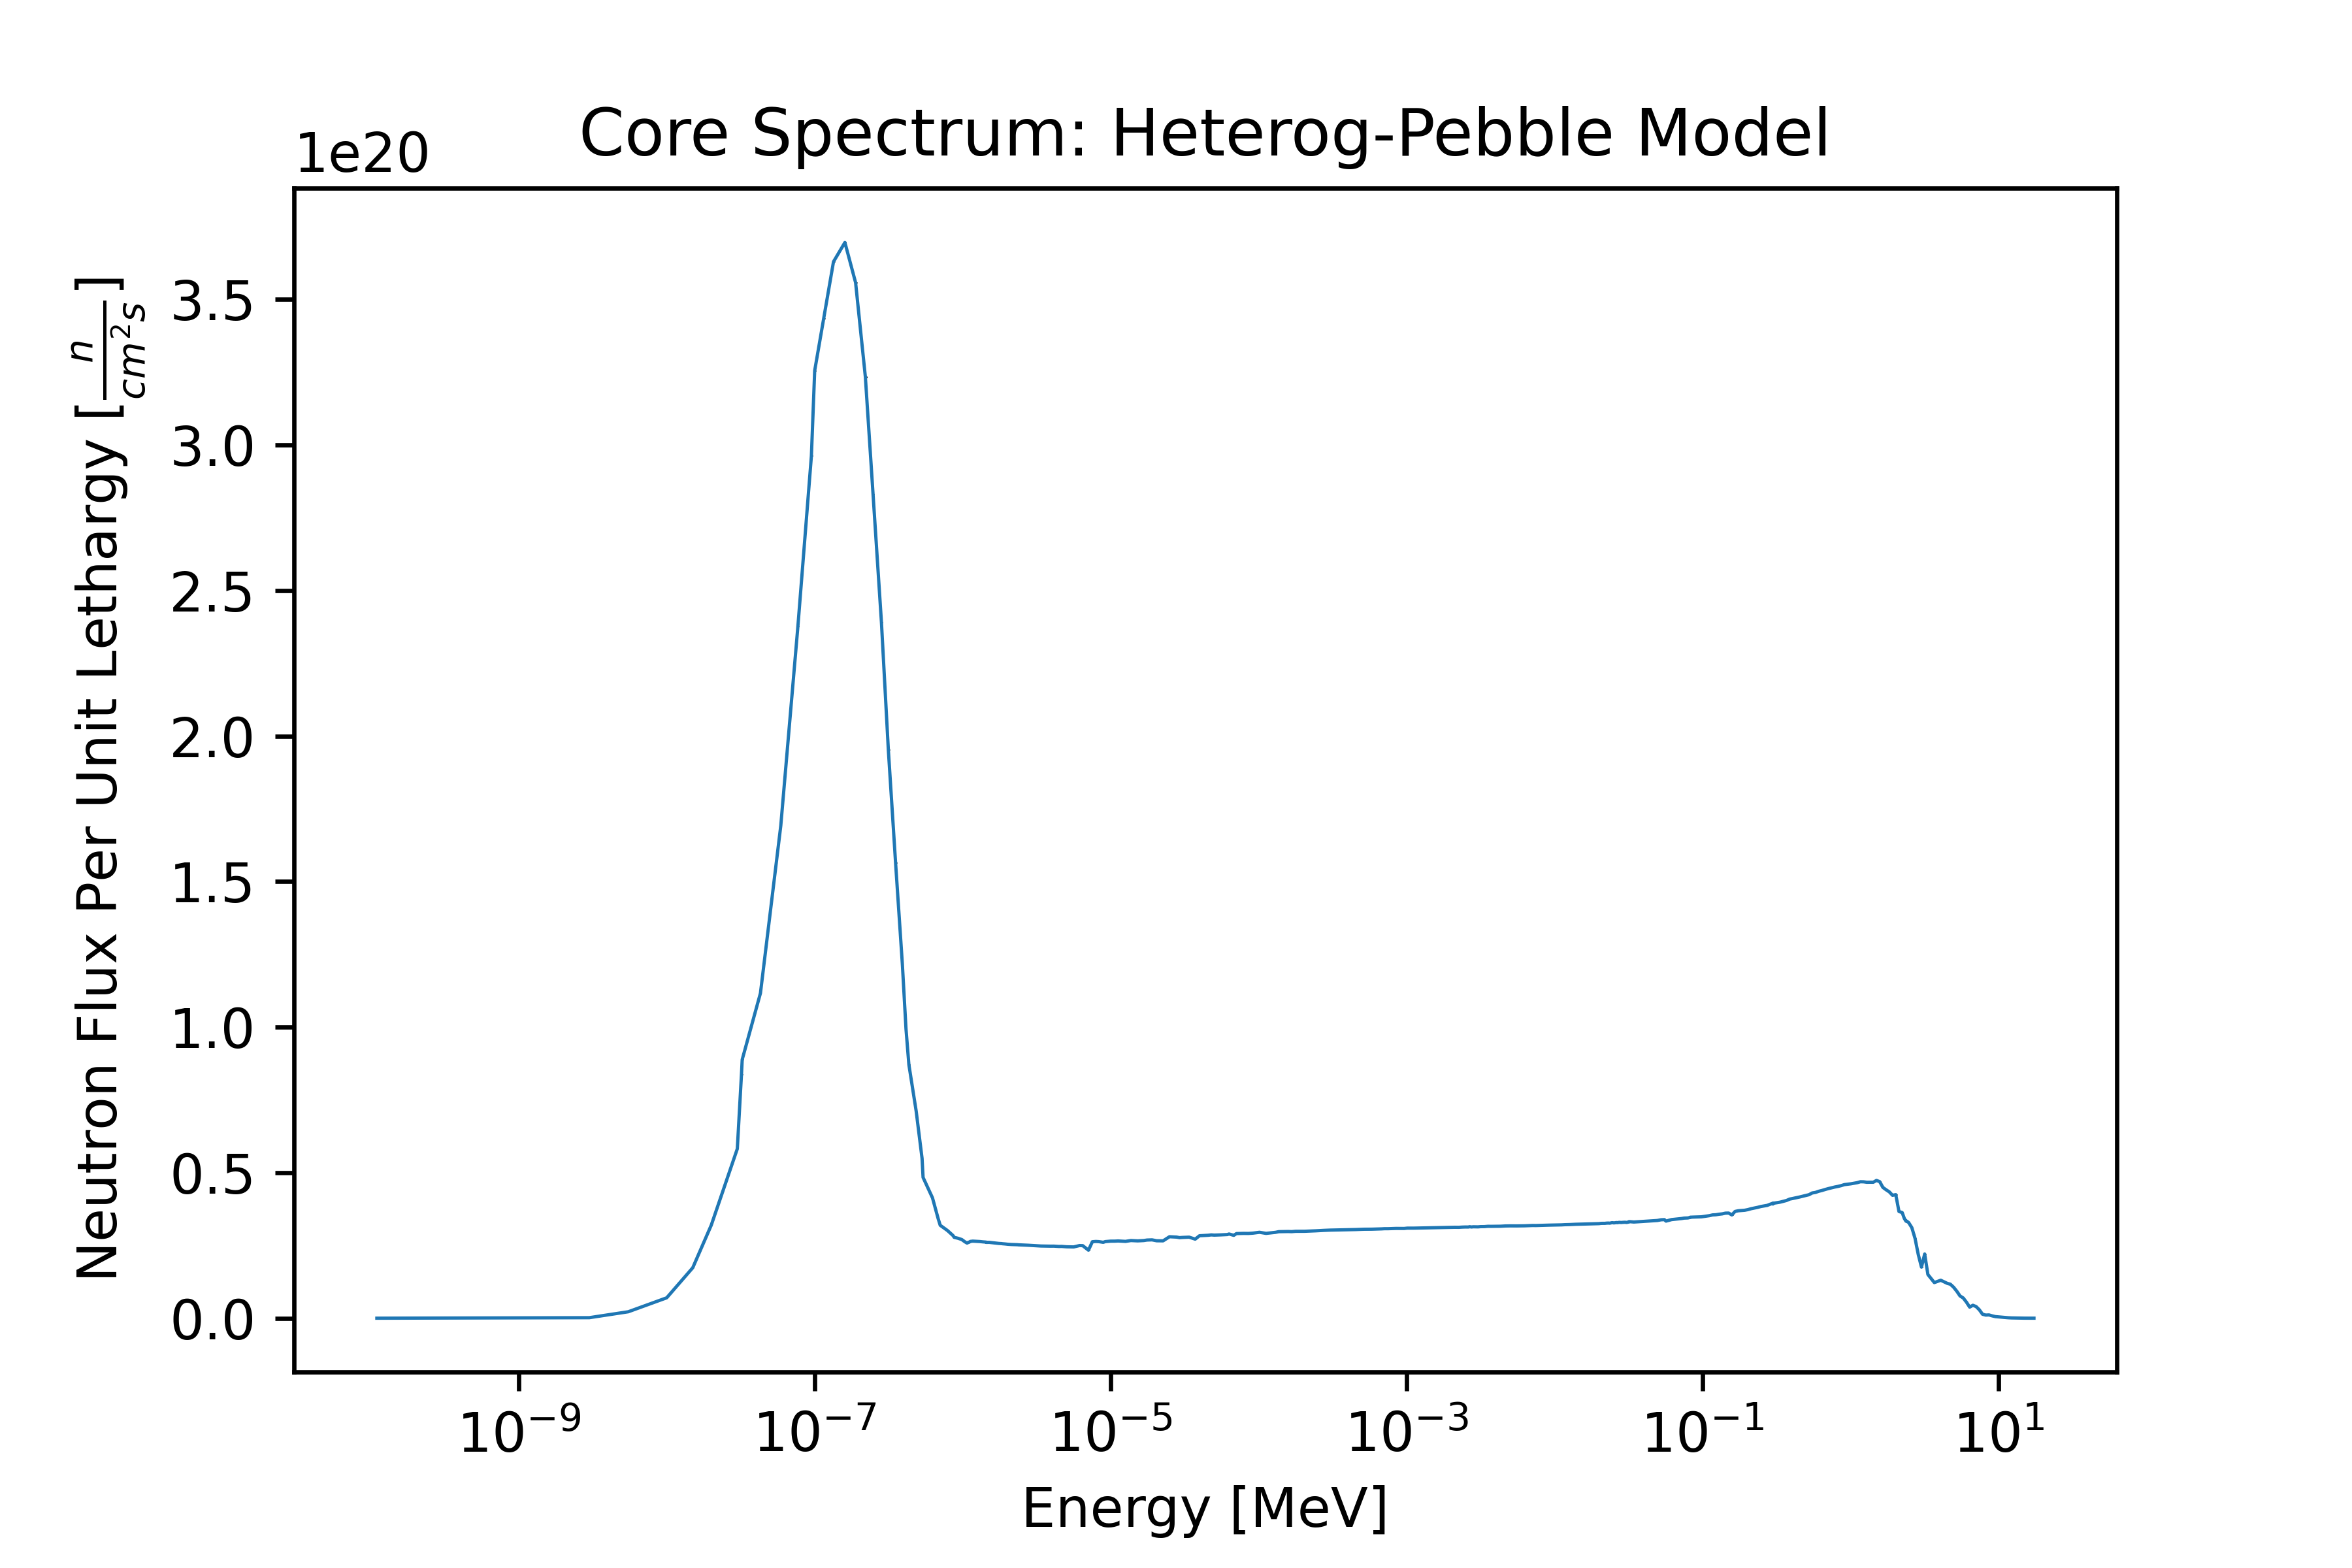
\includegraphics[width=0.95\linewidth]{figures/core_spec_het}
  \caption{Core Spectrum}
  \label{fig:het-core}
\end{subfigure}%

\caption{Lethargy Adjusted Neutron Flux Energy Spectra: Core Using Heterogenized Pebbles}
\end{figure}

\begin{figure}[H]\ContinuedFloat
\centering

\begin{subfigure}{0.95\textwidth}
  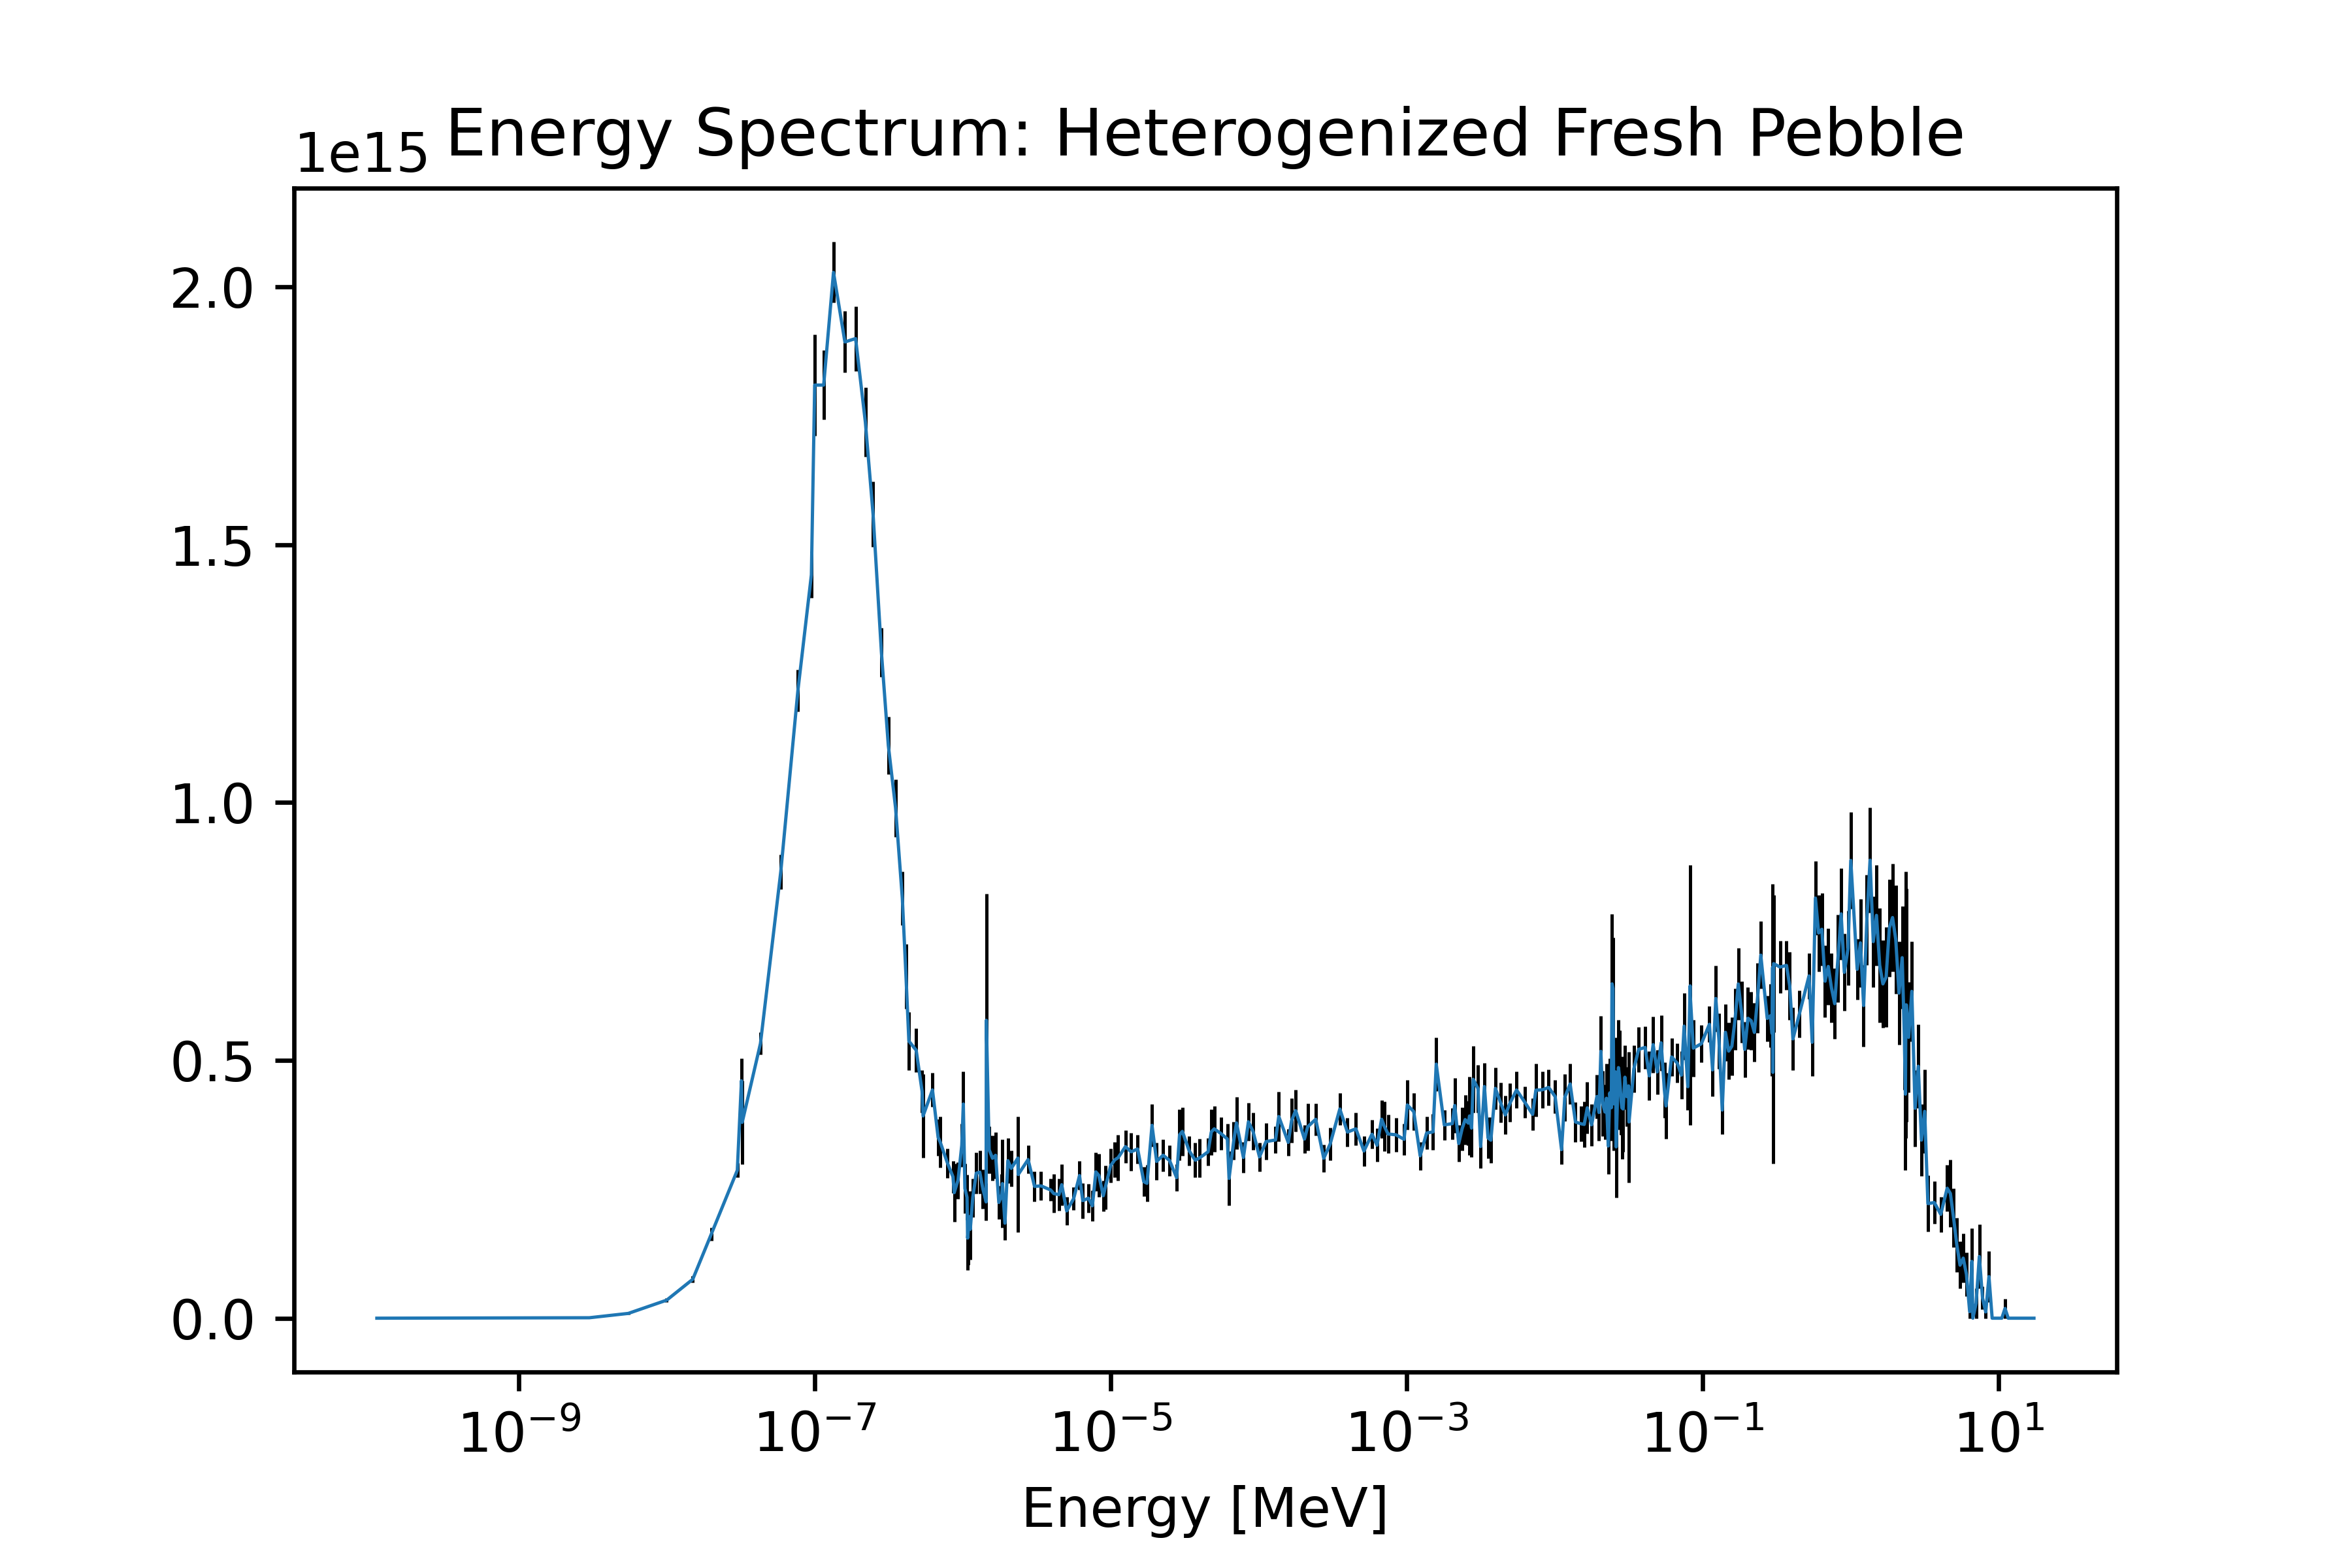
\includegraphics[width=0.95\linewidth]{figures/fresh_spec_het}
  \caption{Fresh Pebble Spectrum}
  \label{fig:het-fresh}
\end{subfigure}%


\begin{subfigure}{0.95\textwidth}
  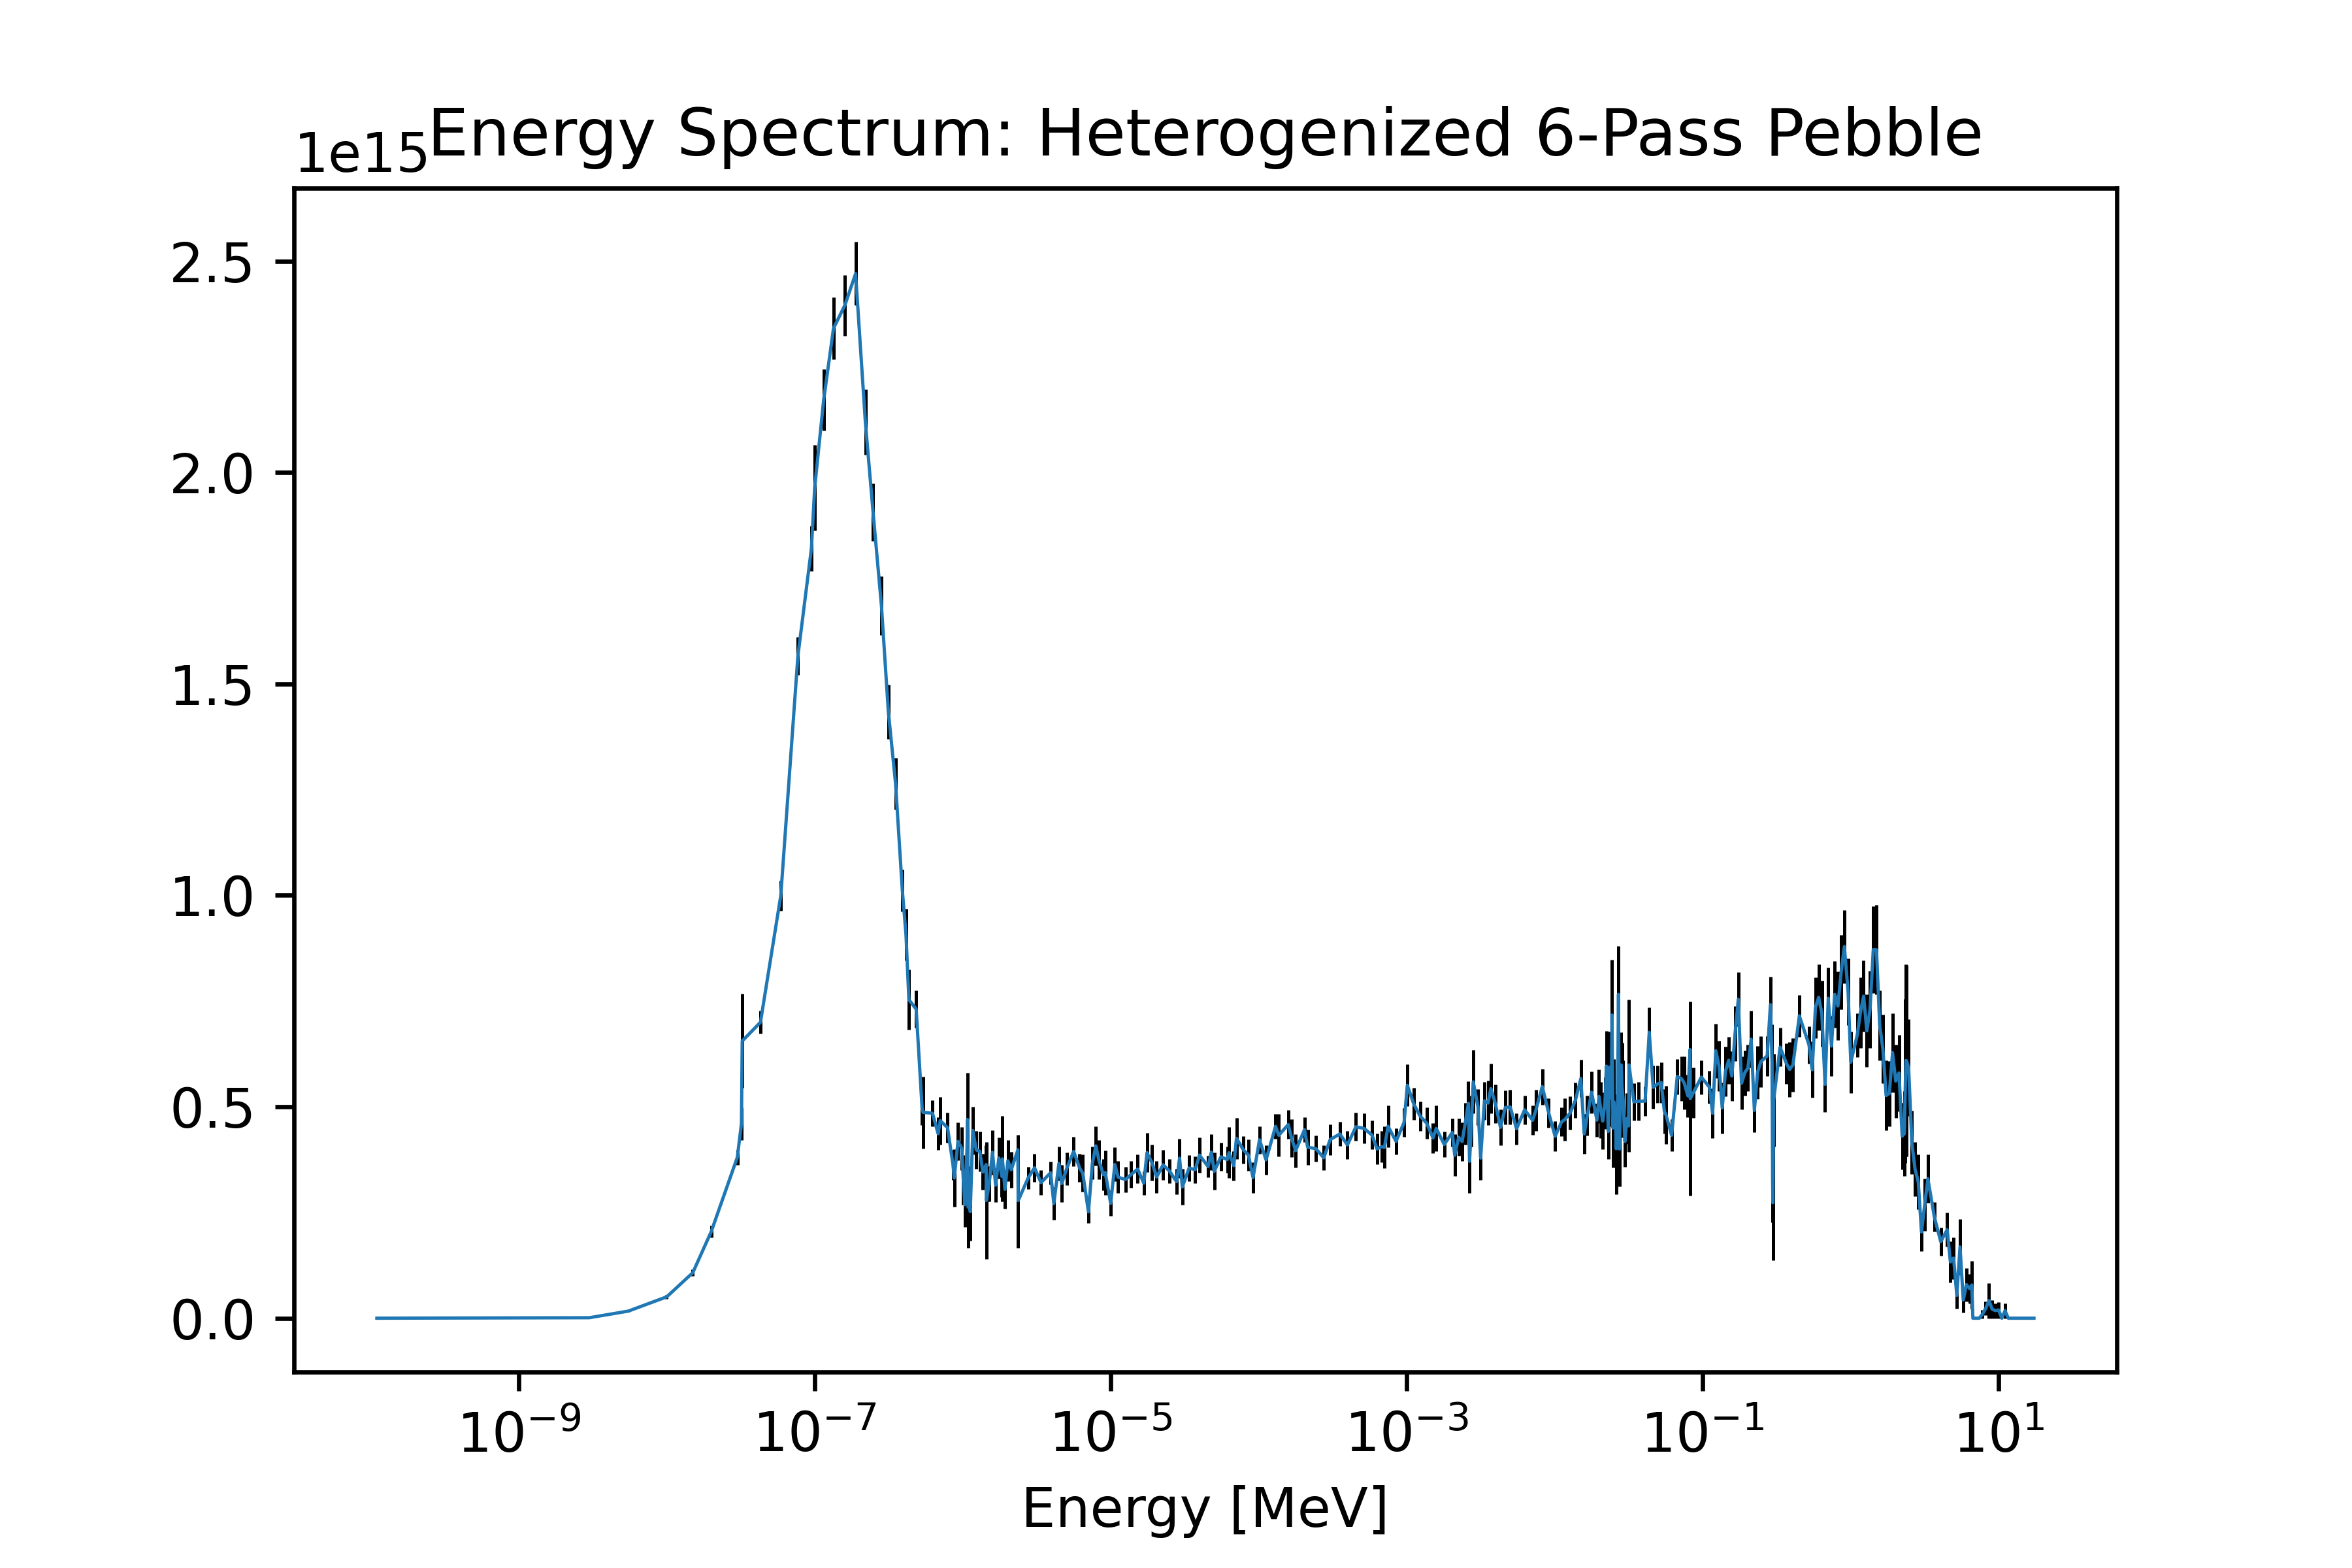
\includegraphics[width=0.95\linewidth]{figures/6_spec_het}
  \caption{Six-Pass Pebble Spectrum}
  \label{fig:het-six}
\end{subfigure}%

\caption{Lethargy Adjusted Neutron Flux Energy Spectra: Core Using Heterogenized Pebbles (cont.)}
\end{figure}

\begin{figure}[H]\ContinuedFloat
\centering

\begin{subfigure}{0.95\textwidth}
  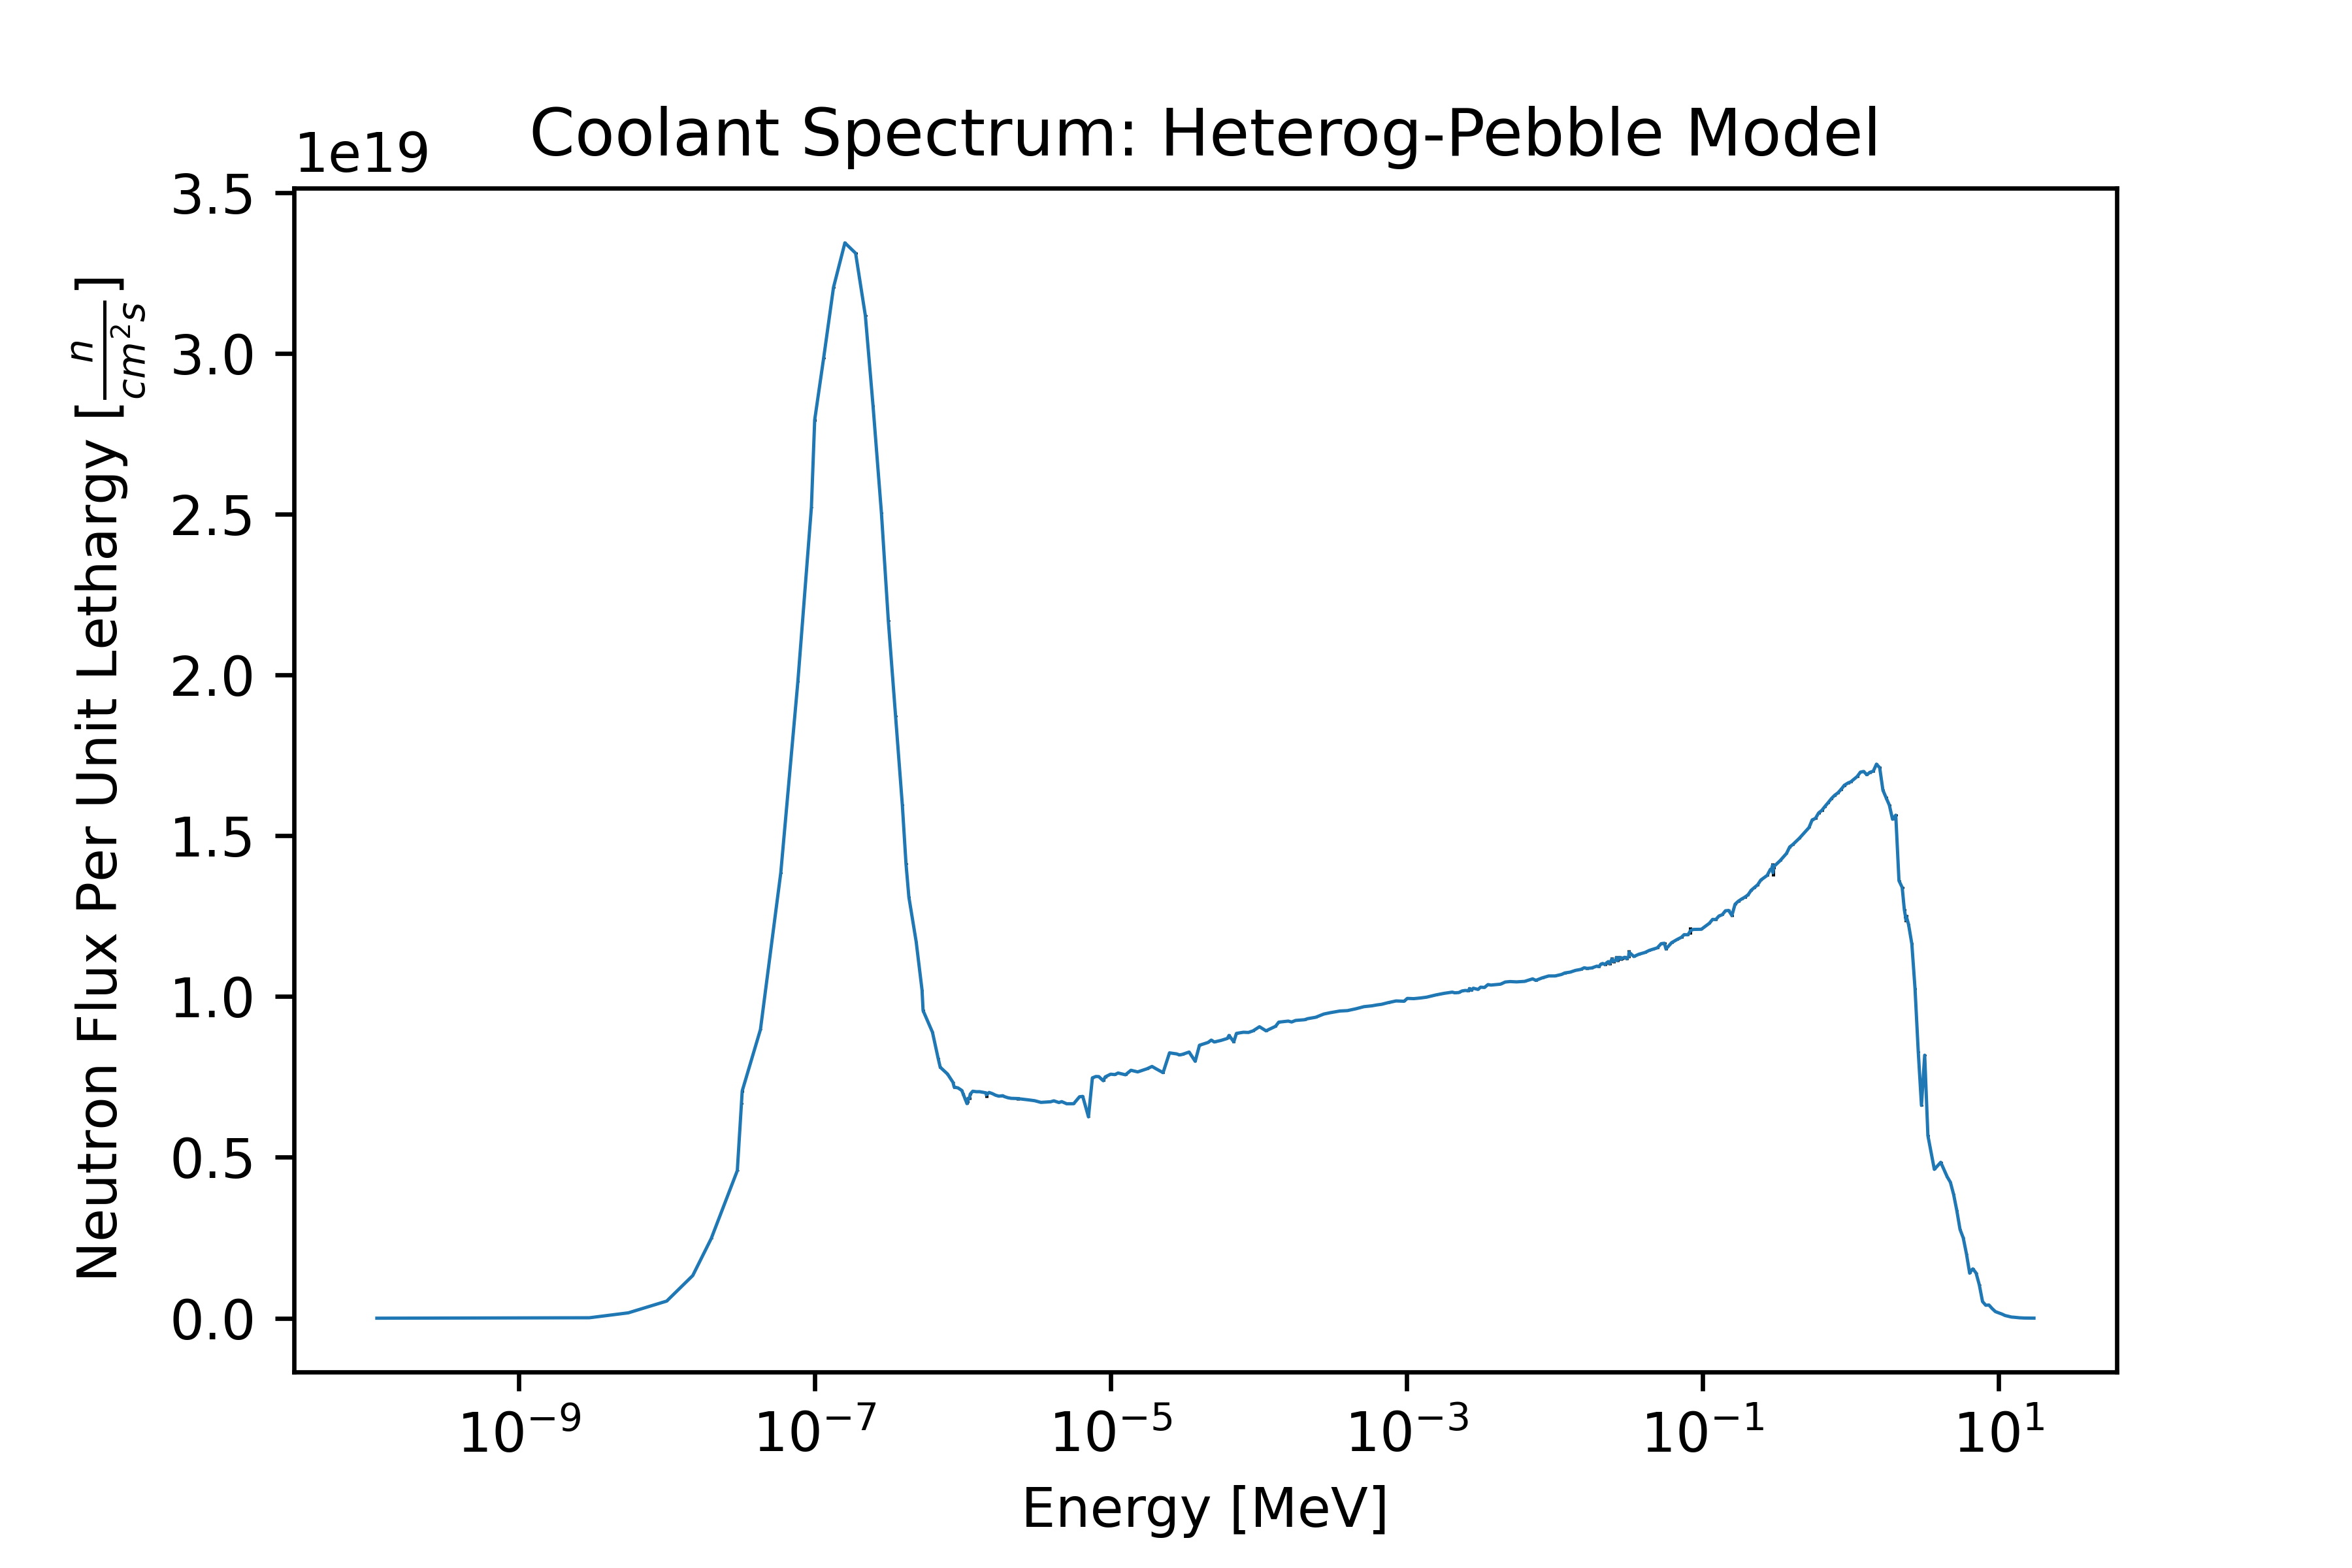
\includegraphics[width=0.95\linewidth]{figures/cool_spec_het}
  \caption{Coolant Spectrum}
  \label{fig:het-cool}
\end{subfigure}%


\begin{subfigure}{0.95\textwidth}
  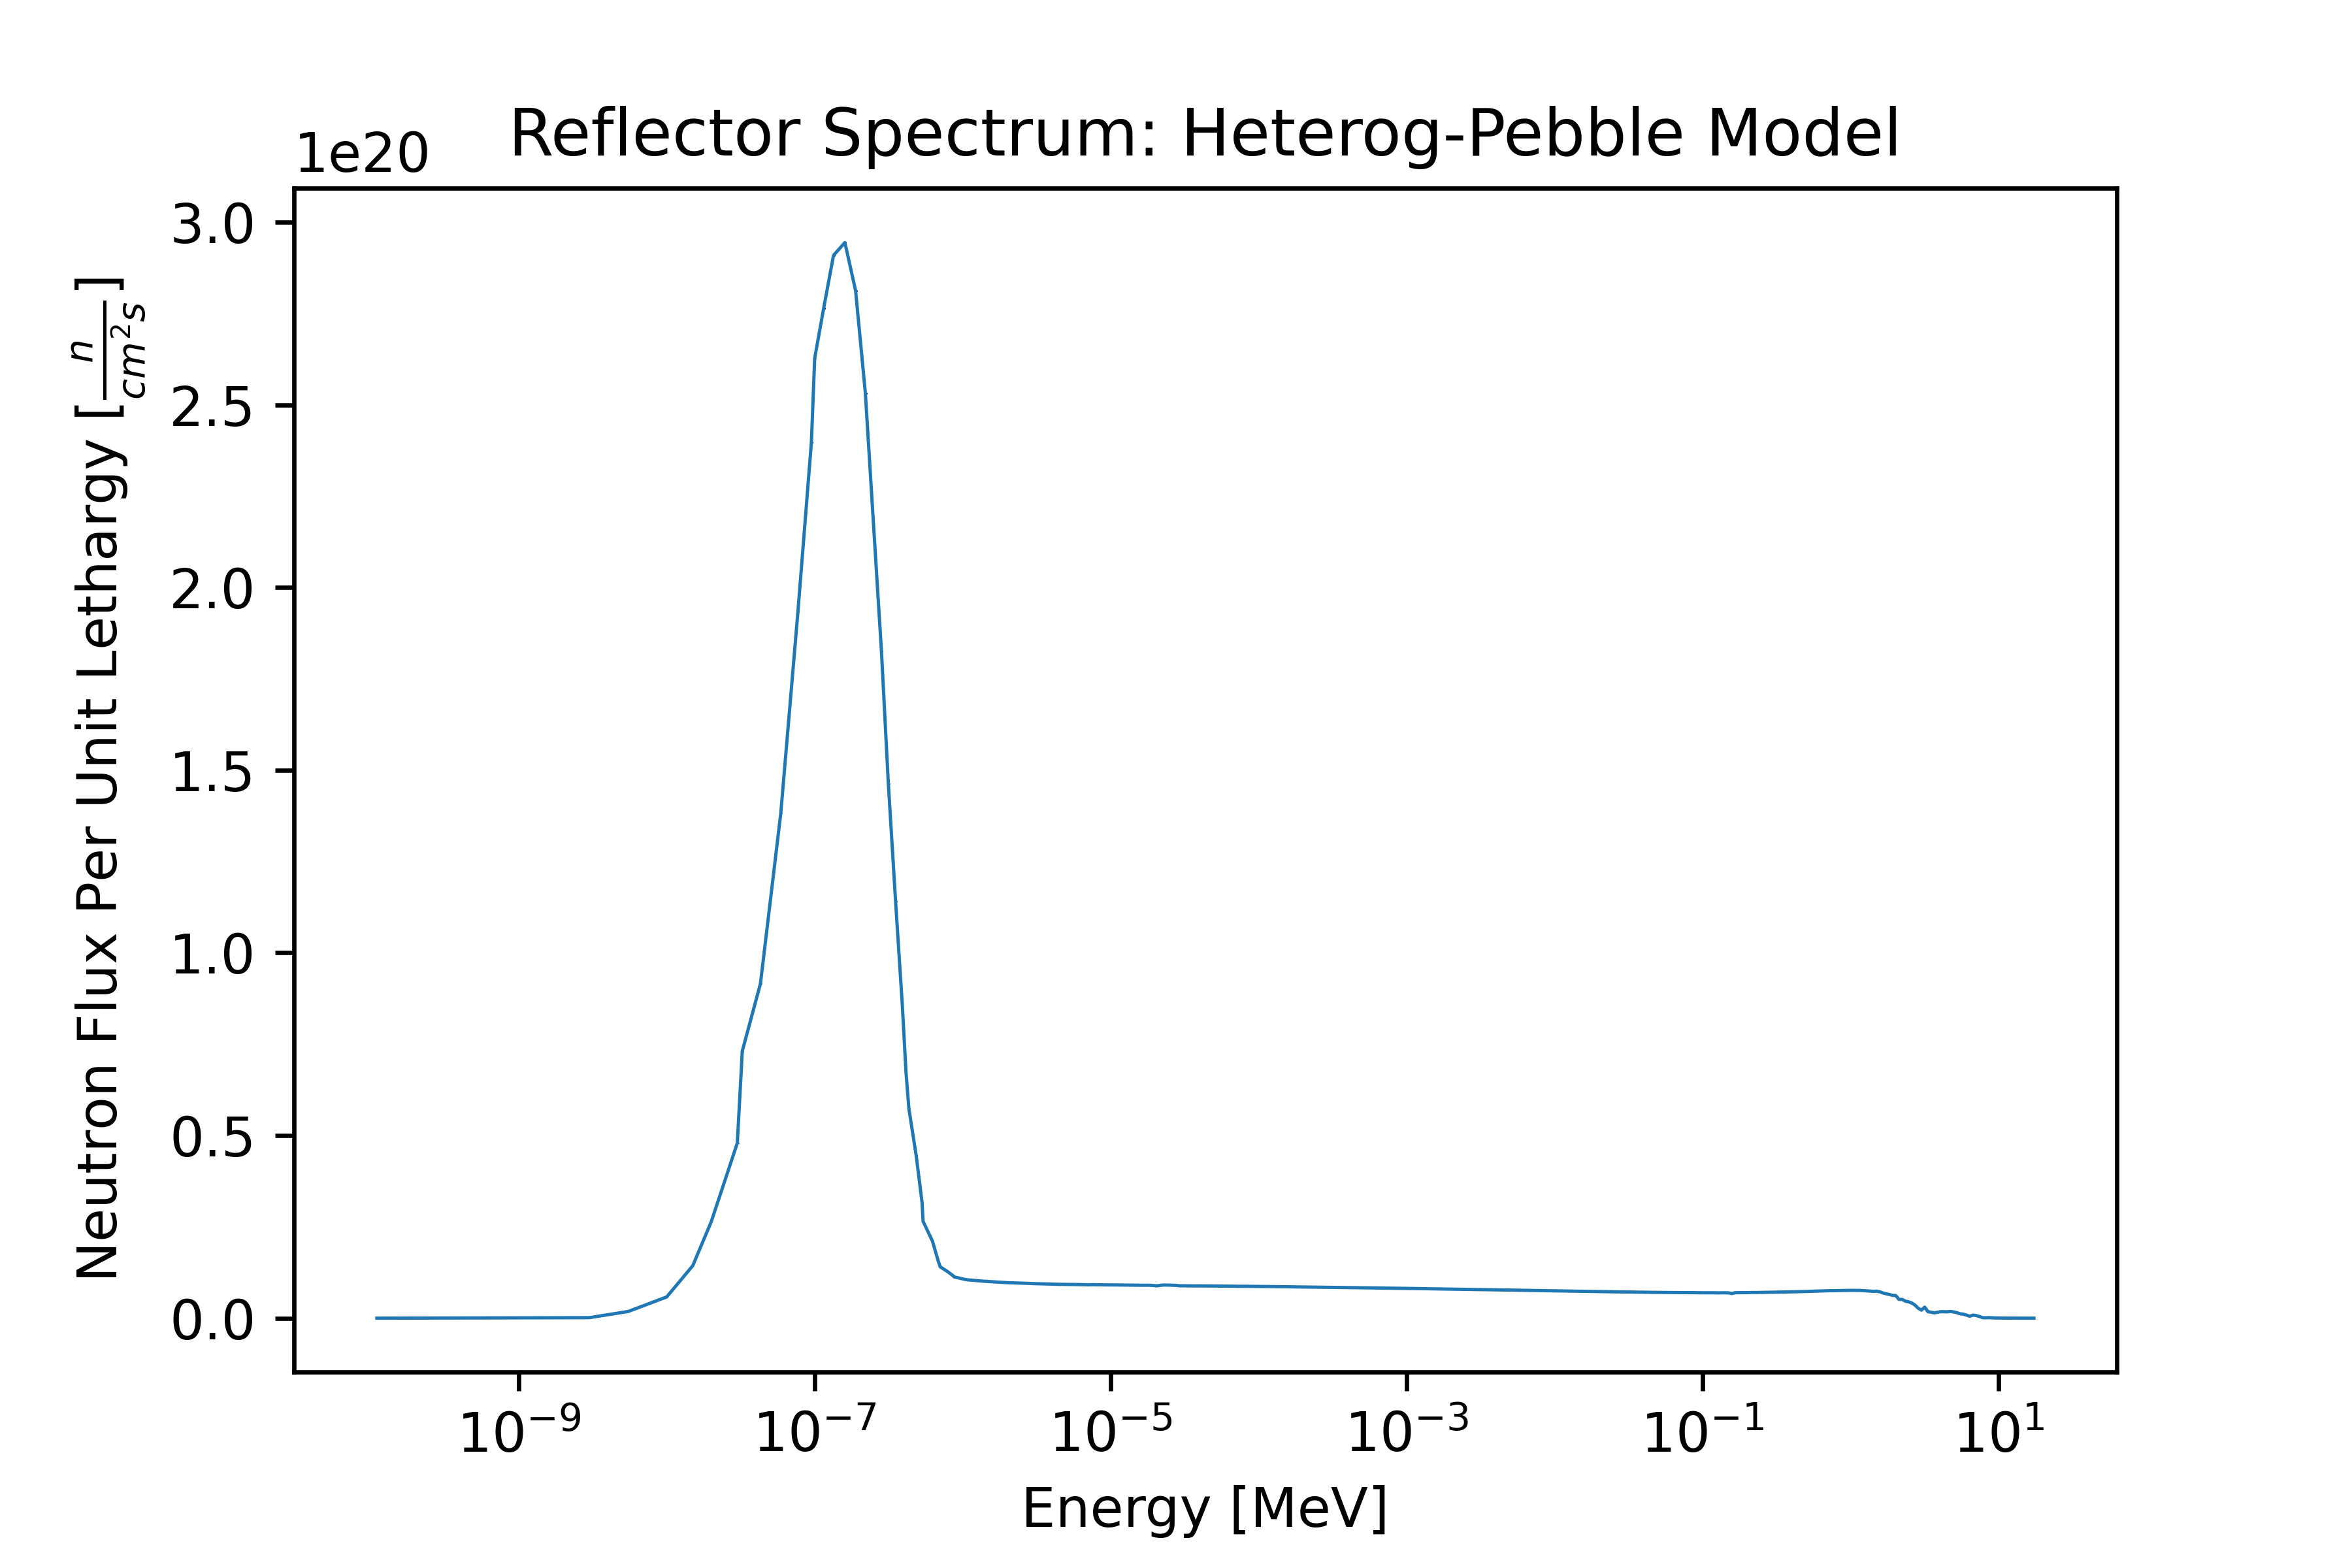
\includegraphics[width=0.95\linewidth]{figures/reflect_spec_het}
  \caption{Reflector Spectrum}
  \label{fig:het-reflec}
\end{subfigure}%


\caption{Lethargy Adjusted Neutron Flux Energy Spectra: Core Using Heterogenized Pebbles (cont.)}
\label{fig:hom-spec}
\end{figure}

The heterogenized spectra, much like the flux profiles, are of a very similar morphology.  In order to better examine the differences between the homogenized and heterogenized models, simple relative difference was calculated and plotted for all spectra, and the radial fast and thermal profiles.  The relative difference was calculated according to the following:

\begin{align}
\Delta i &= \frac{i_{hom} - i_{het}}{i_{het}}
\intertext{where}
\Delta i&= \mbox{ relative difference for parameter i between homogenized and heterogenized model }\nonumber\\
i_{hom}&= \mbox{ homogenized parameter i}\nonumber\\
i_{het}&= \mbox{ heterogenized parameter i}\nonumber\\
\end{align}

And error was calculated using simple error propagation rules.


\begin{figure}[H]
\centering

\begin{subfigure}{0.9\textwidth}
  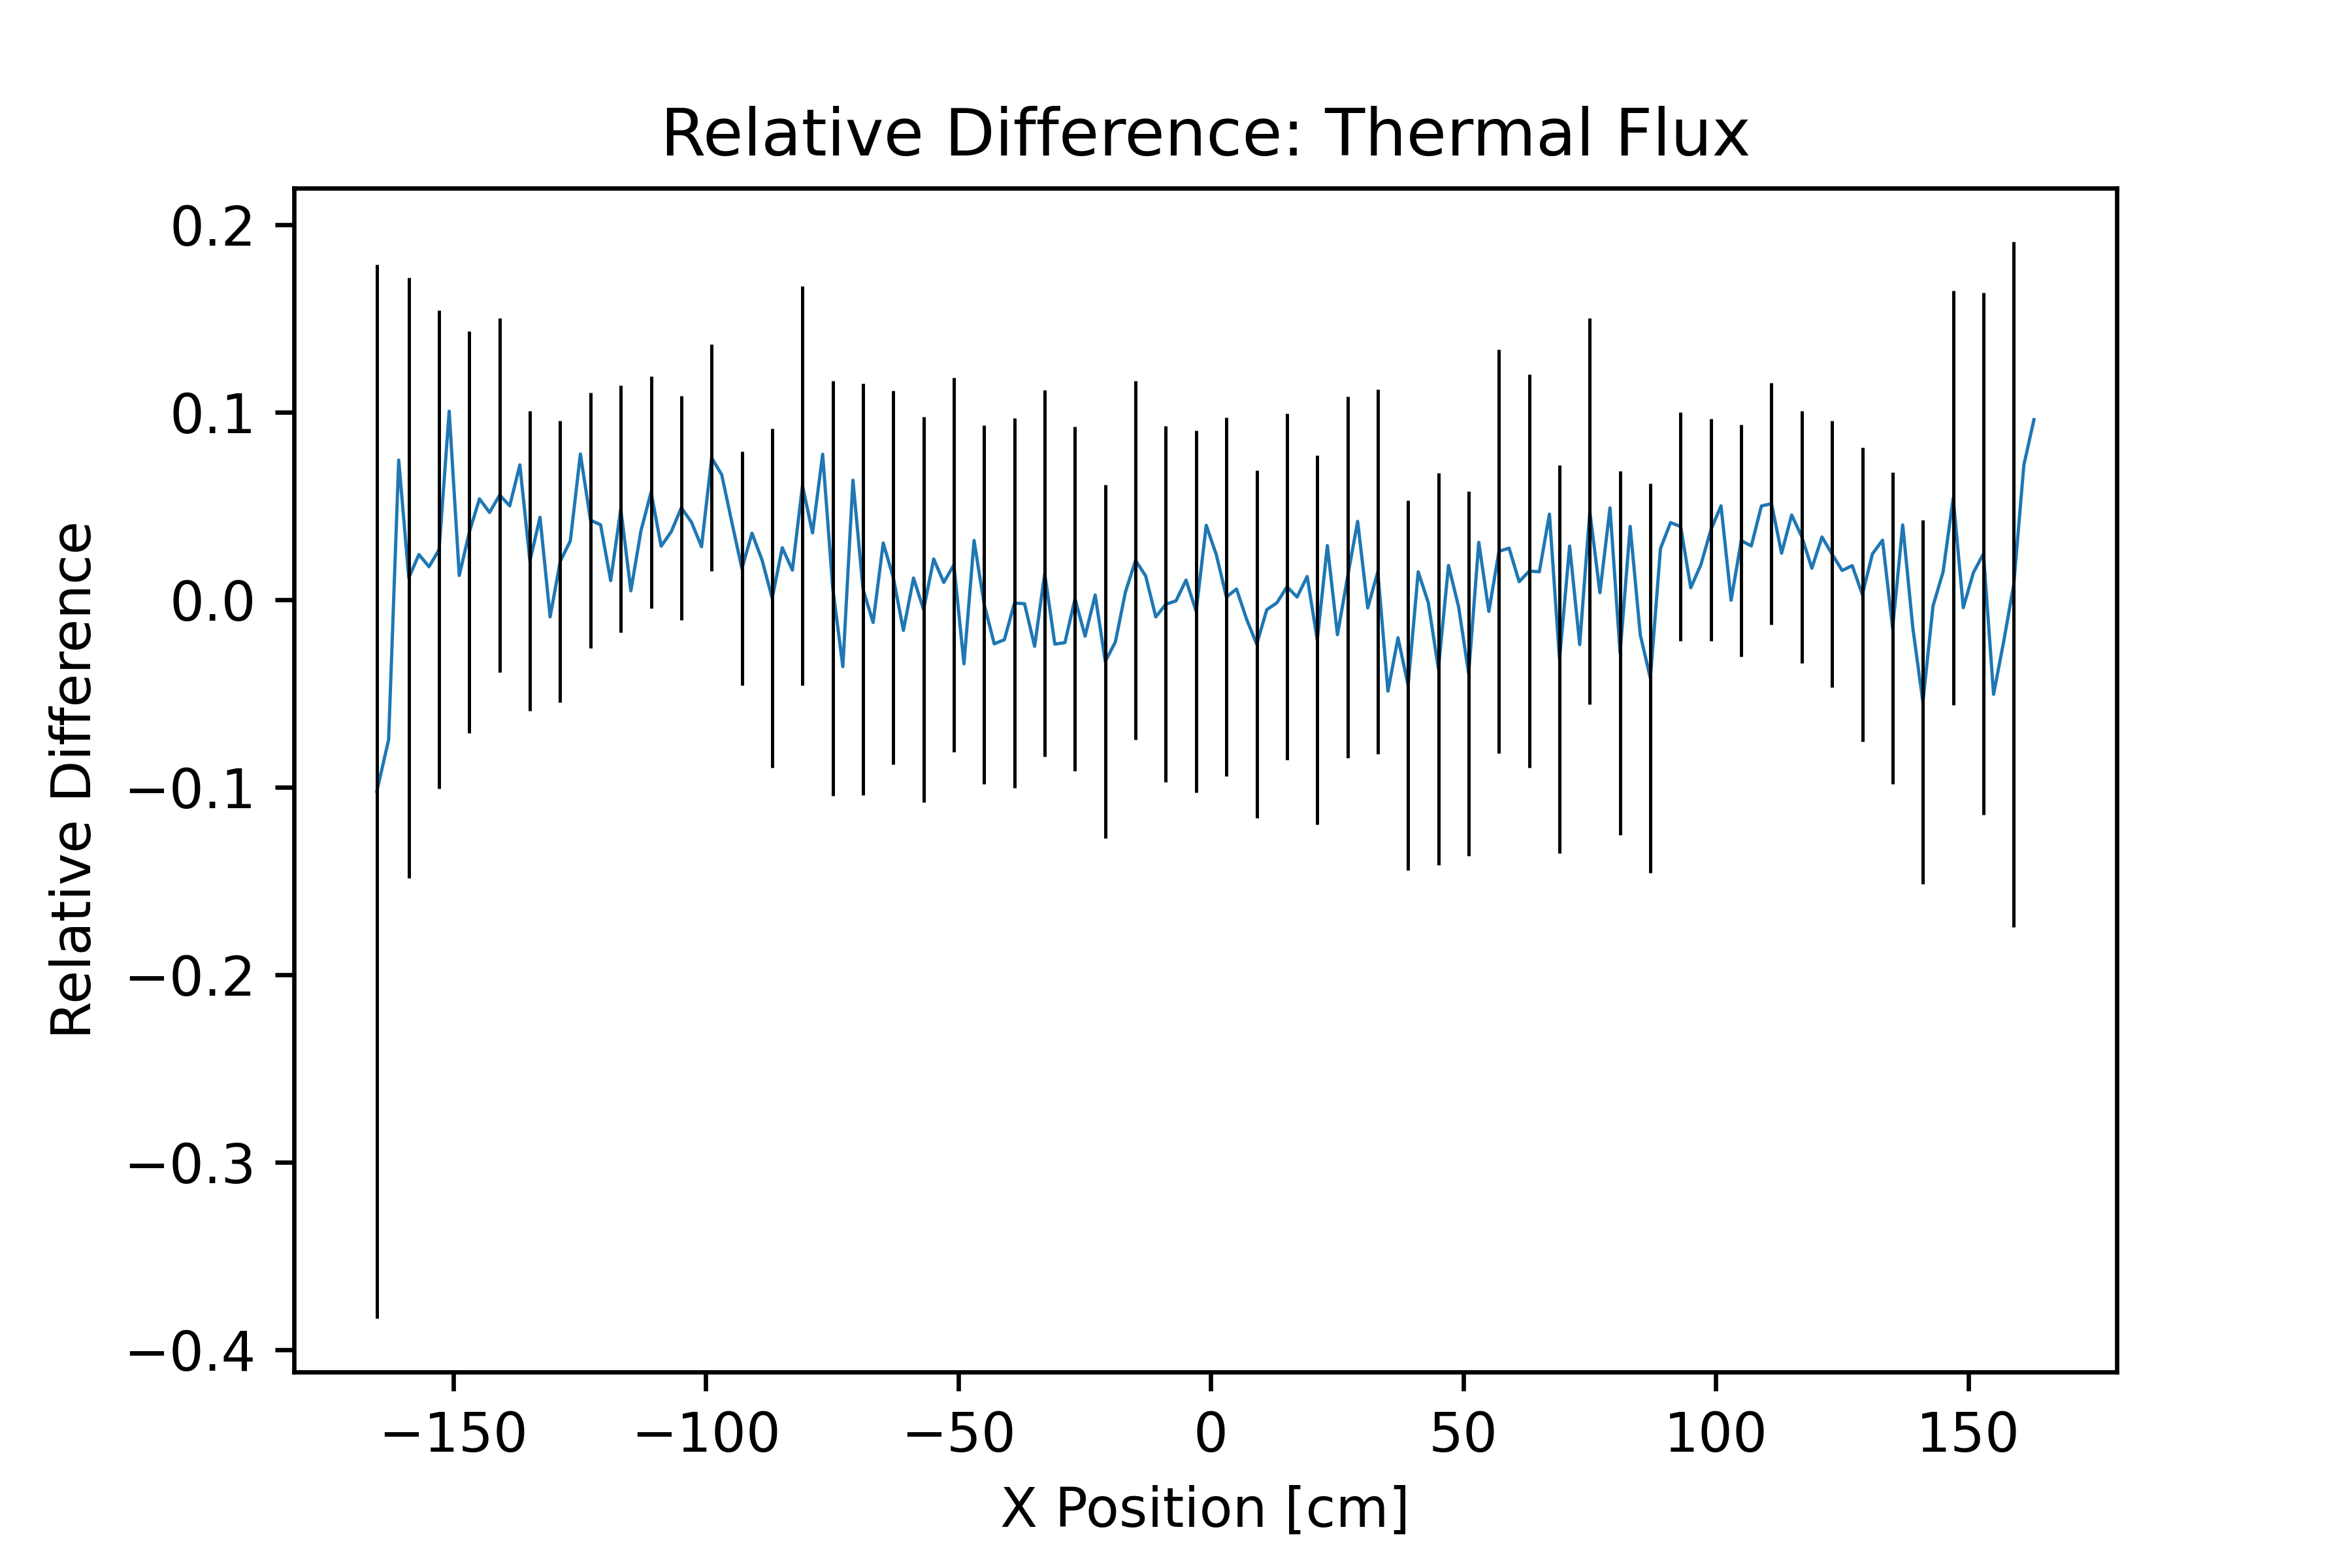
\includegraphics[width=0.9\linewidth]{figures/reldiff_therm_flux.png}
  \caption{Thermal Flux}
  \label{fig:diff-therm}
\end{subfigure}%

\caption{Relative Difference in Radial Thermal and Fast Flux Profiles Between Cores Using Homogenized and Heterogenized Pebbles}
\end{figure}

\begin{figure}[H]\ContinuedFloat
\centering

\begin{subfigure}{0.9\textwidth}
  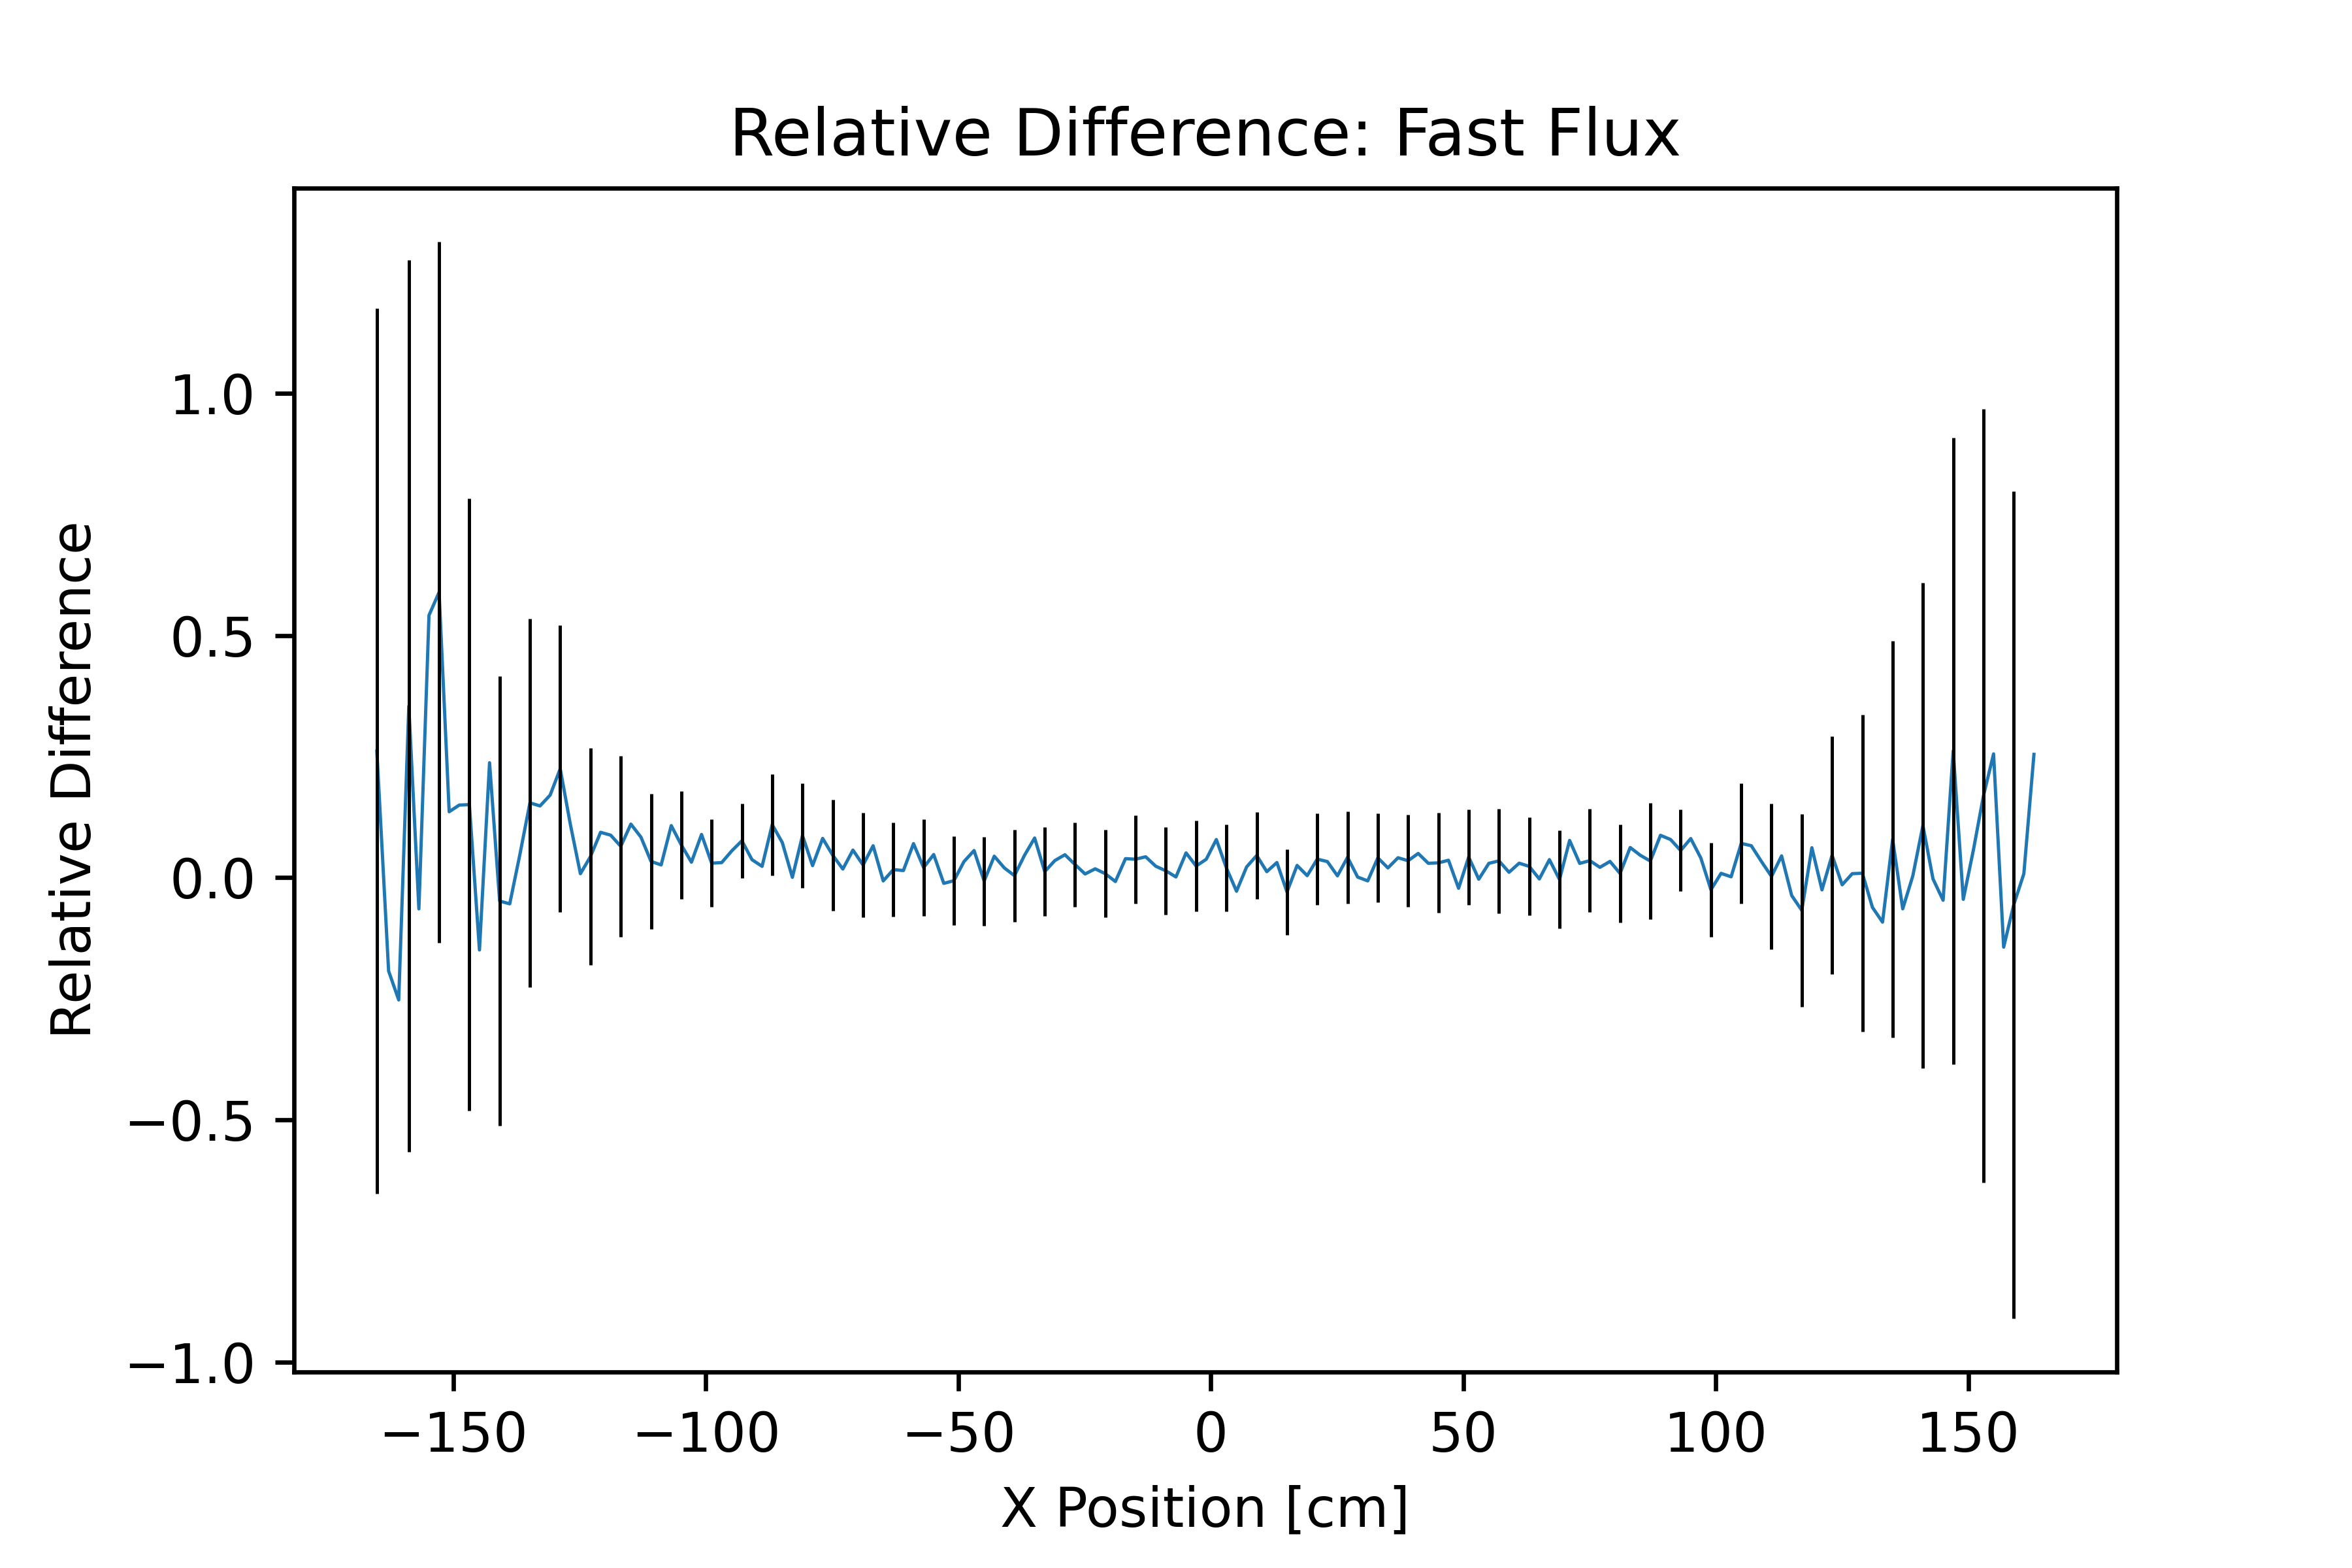
\includegraphics[width=0.9\linewidth]{figures/reldiff_fast_flux.png}
  \caption{Fast Flux}
  \label{fig:diff-fast}
\end{subfigure}

%
\caption[]{(cont.)}
\label{fig:diff-flux}
\end{figure}

For both the thermal and flux profiles, the higher error at the edges of the flux profile is exacerbated.  Overall, \ref{fig:diff-therm} and \ref{fig:diff-fast} suggest that the homogenized model is slightly over-predicting the magnitude of the flux, however, given the size of the error, these differences cannot be said to exist with certainty.


\begin{figure}[H]
\centering
%
\begin{subfigure}{0.95\textwidth}
  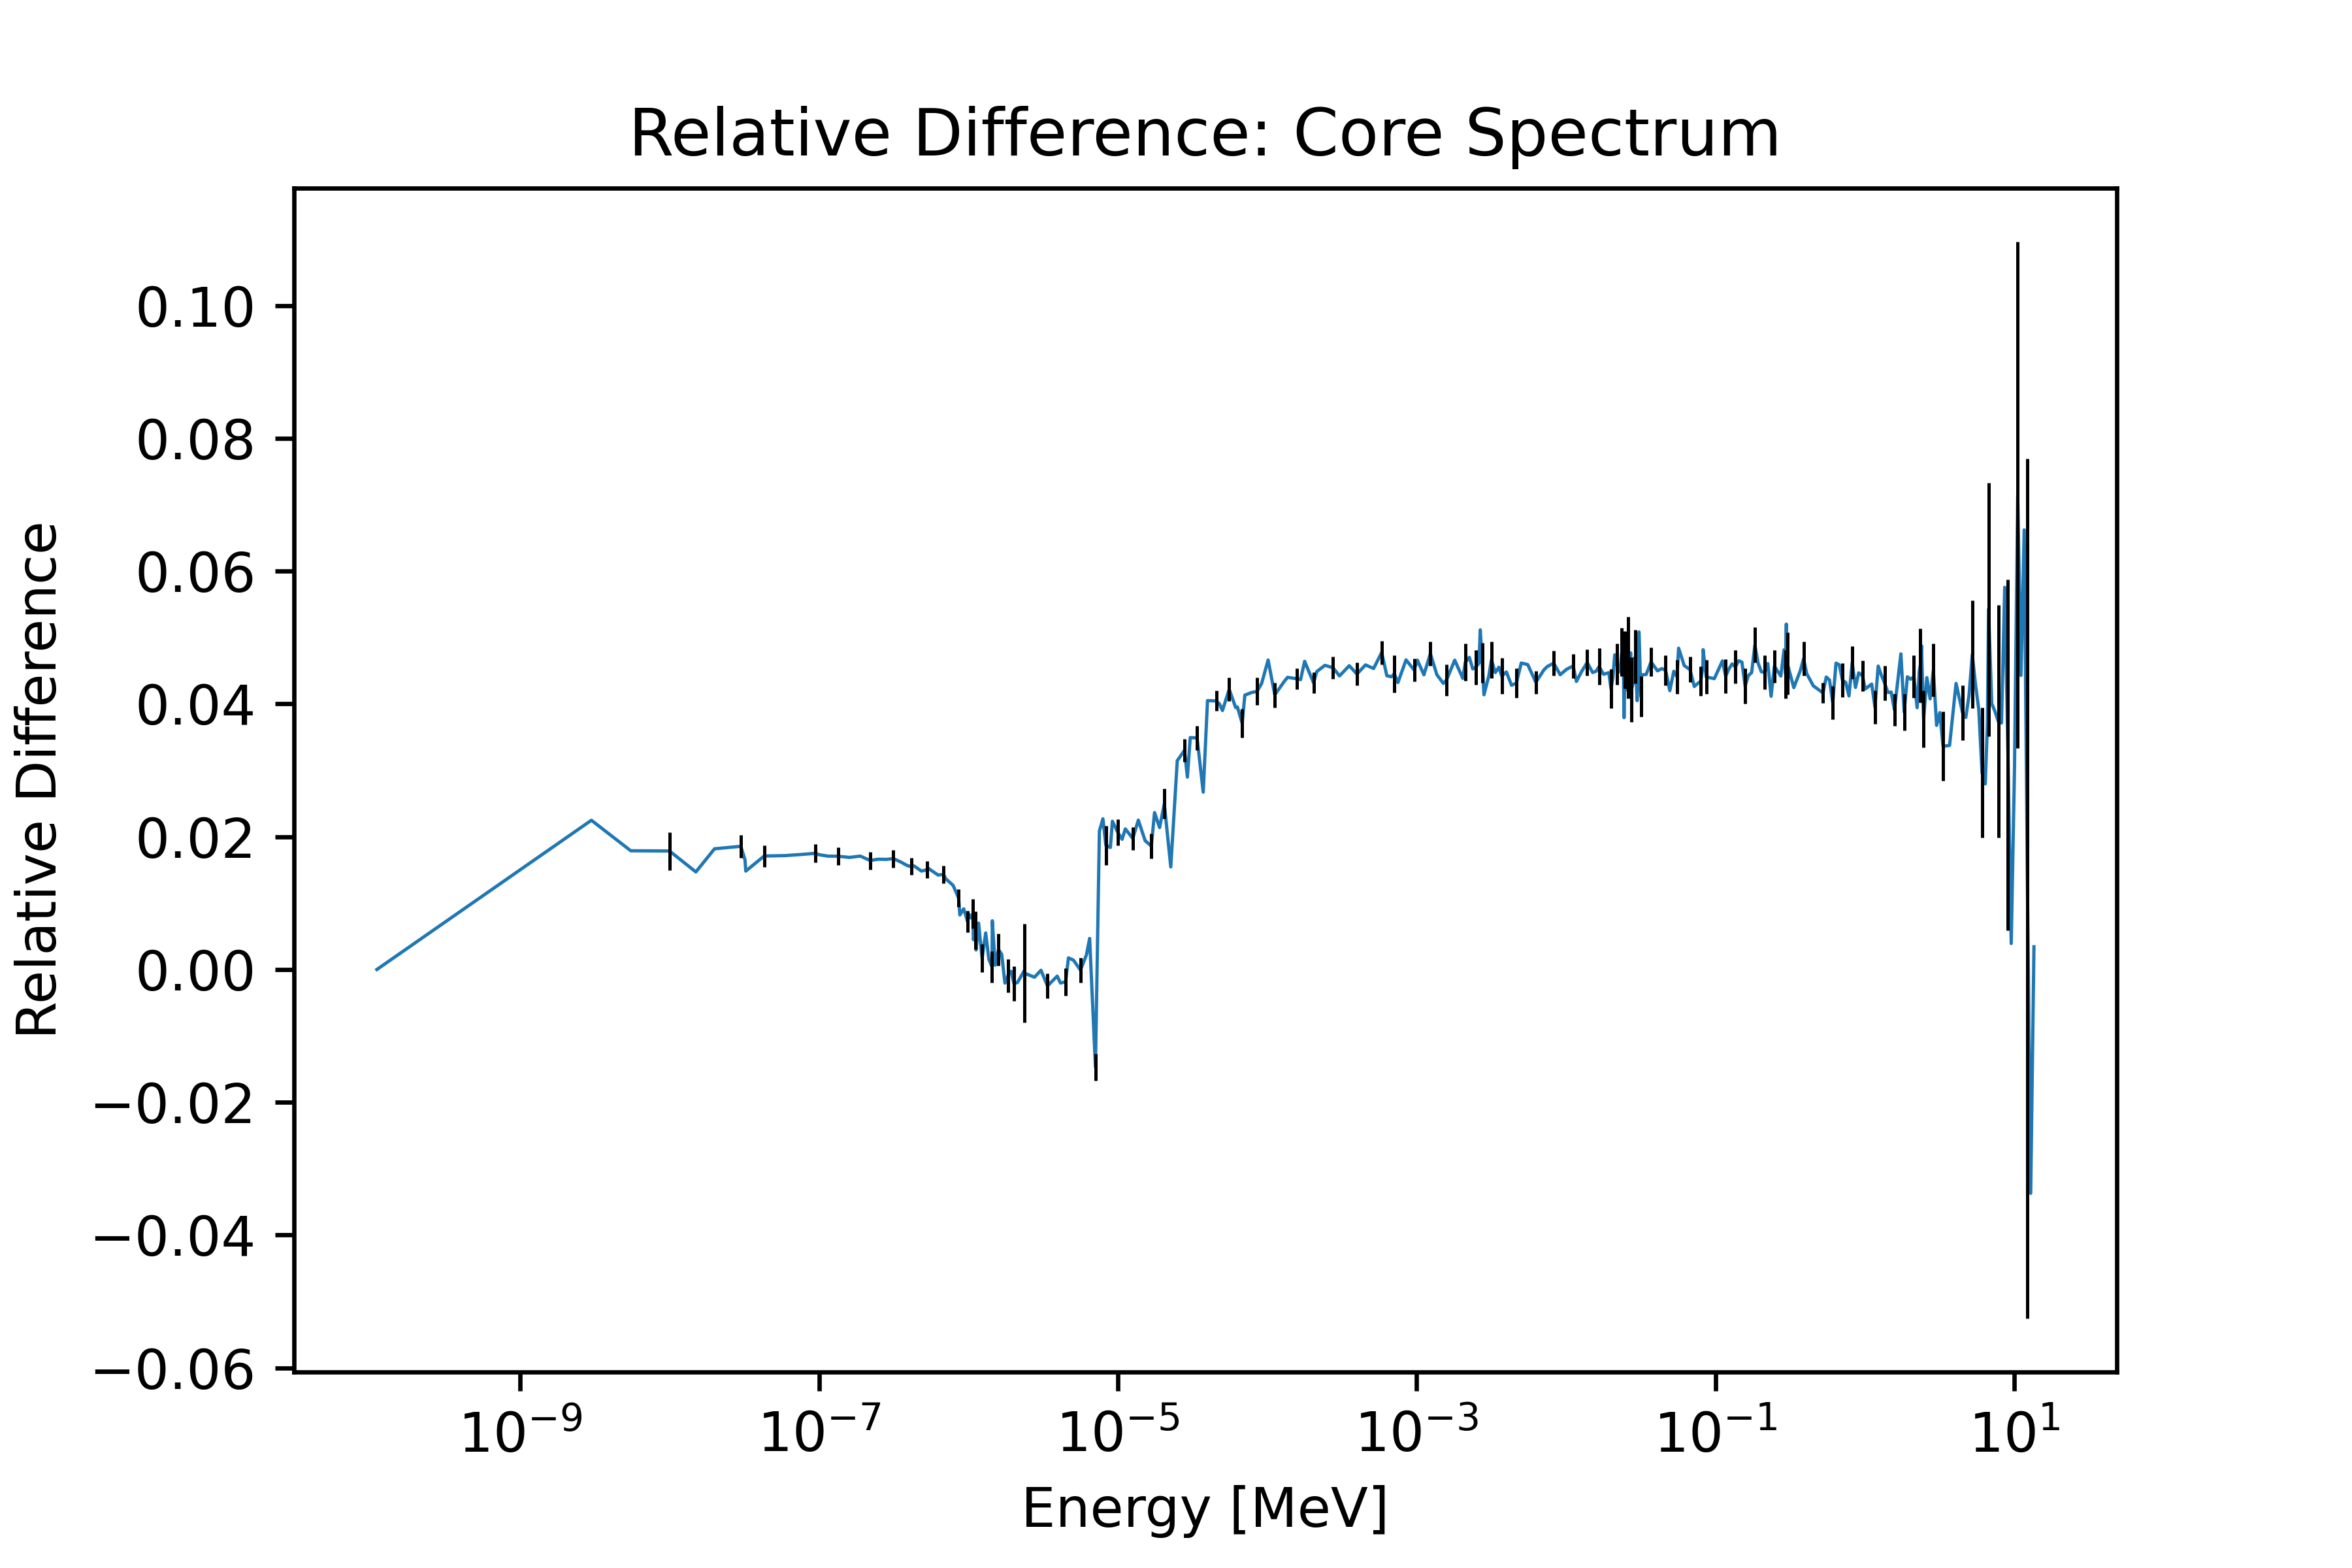
\includegraphics[width=0.95\linewidth]{figures/reldiff_core_spec_er}
  \caption{Core}
  \label{fig:diff-core}
\end{subfigure}%


\begin{subfigure}{0.95\textwidth}
  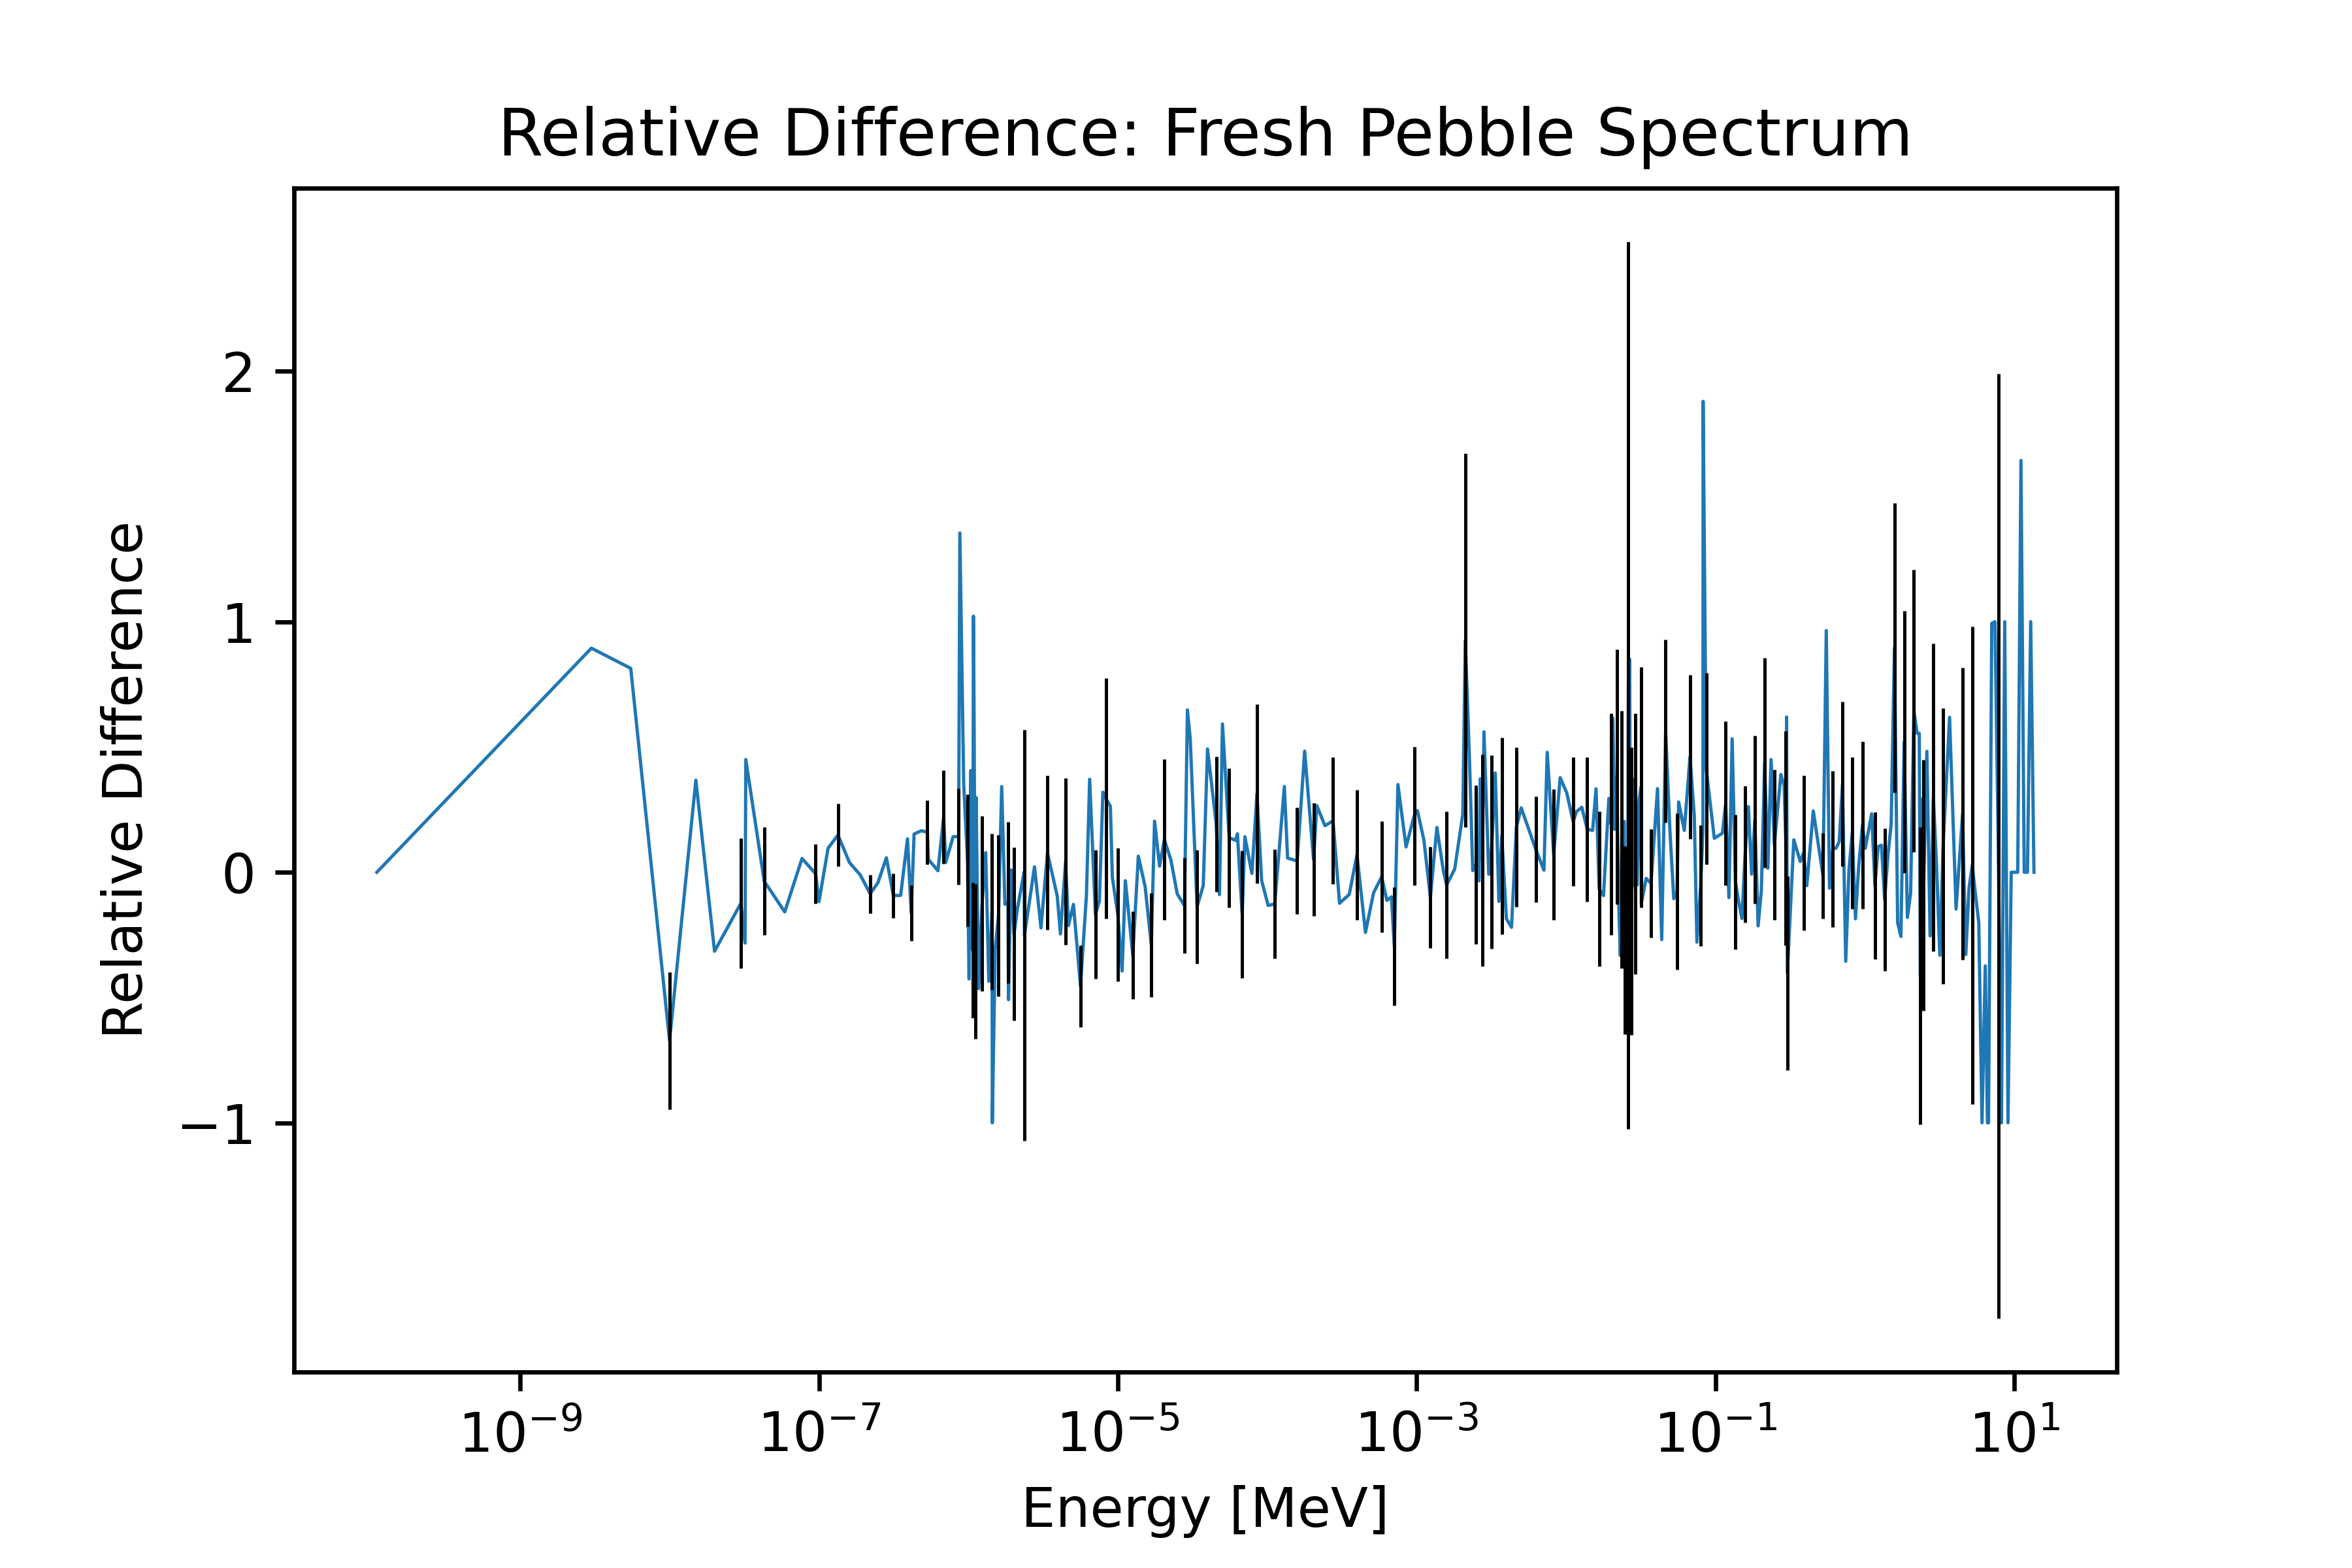
\includegraphics[width=0.95\linewidth]{figures/reldiff_fresh_spec_er}
  \caption{Fresh Pebble}
  \label{fig:diff-fresh}
\end{subfigure}%

\caption{Relative Difference in Lethargy Adjusted Neutron Flux Energy Spectra Between Cores using Homogenized and Heterogenized Pebbles}
\end{figure}

\begin{figure}[H]\ContinuedFloat
\centering

\begin{subfigure}{0.95\textwidth}
  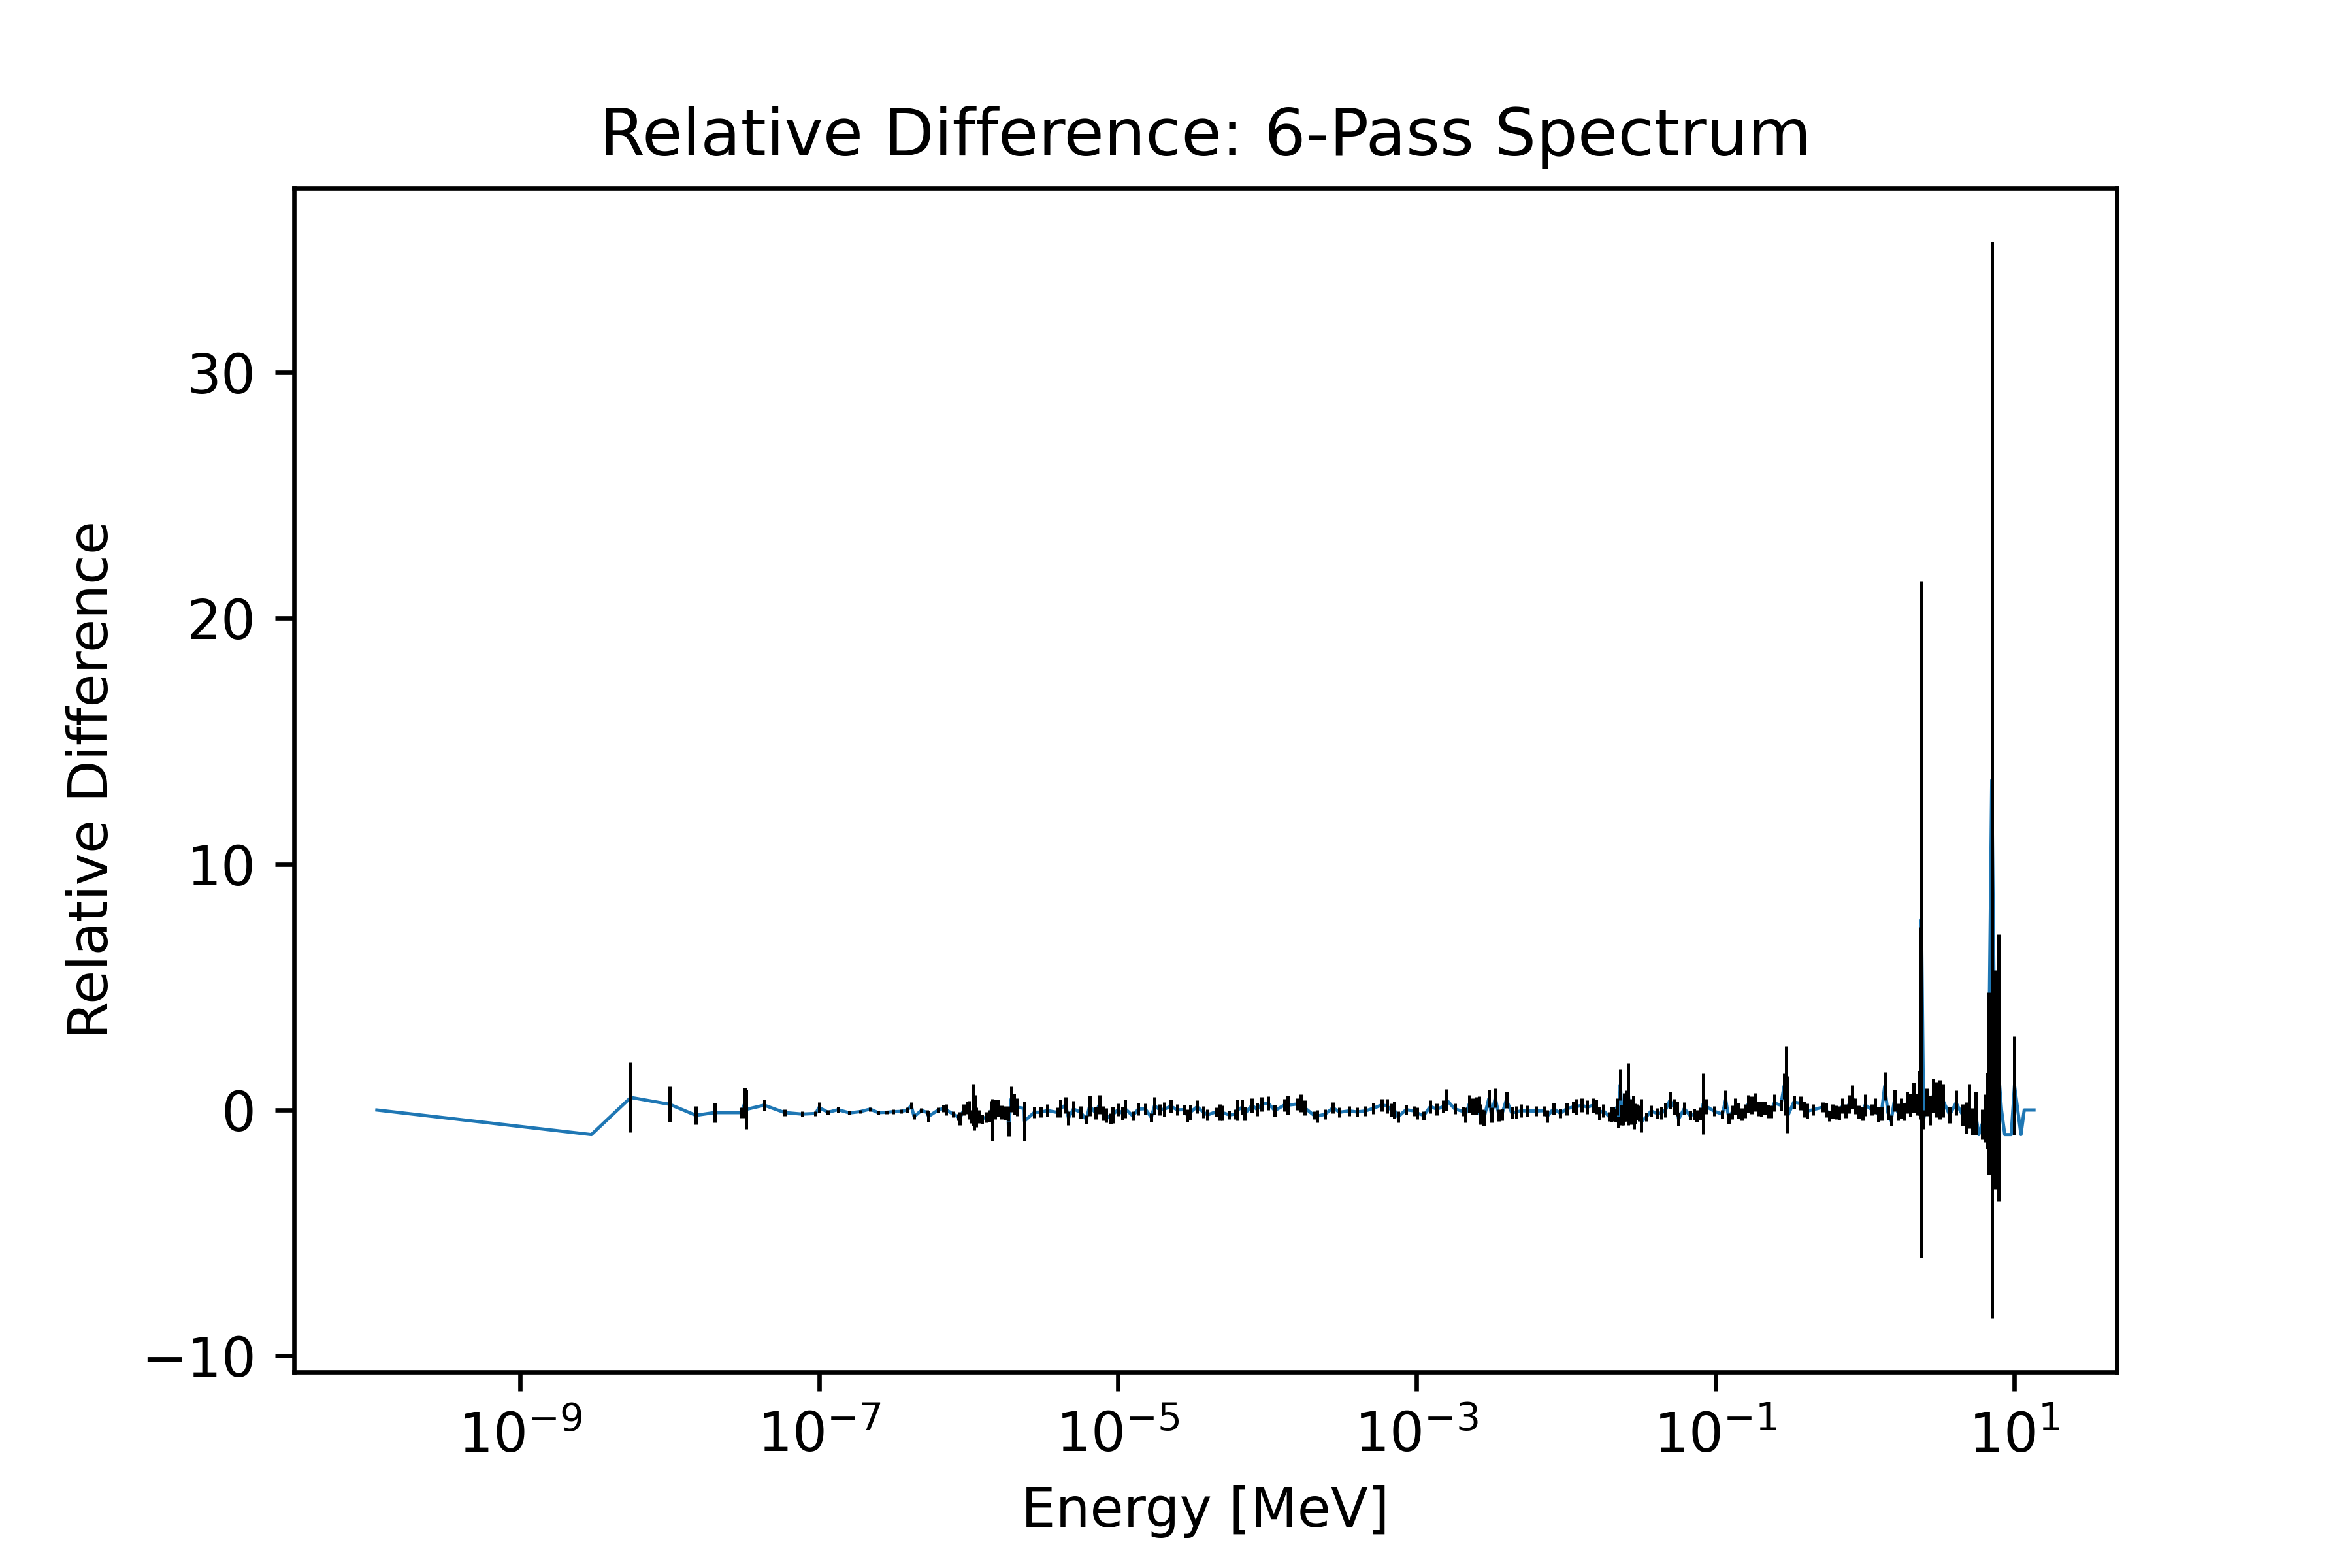
\includegraphics[width=0.95\linewidth]{figures/reldiff_six_spec_er}
  \caption{Six-Pass Pebble}
  \label{fig:diff-six}
\end{subfigure}%


\begin{subfigure}{0.95\textwidth}
  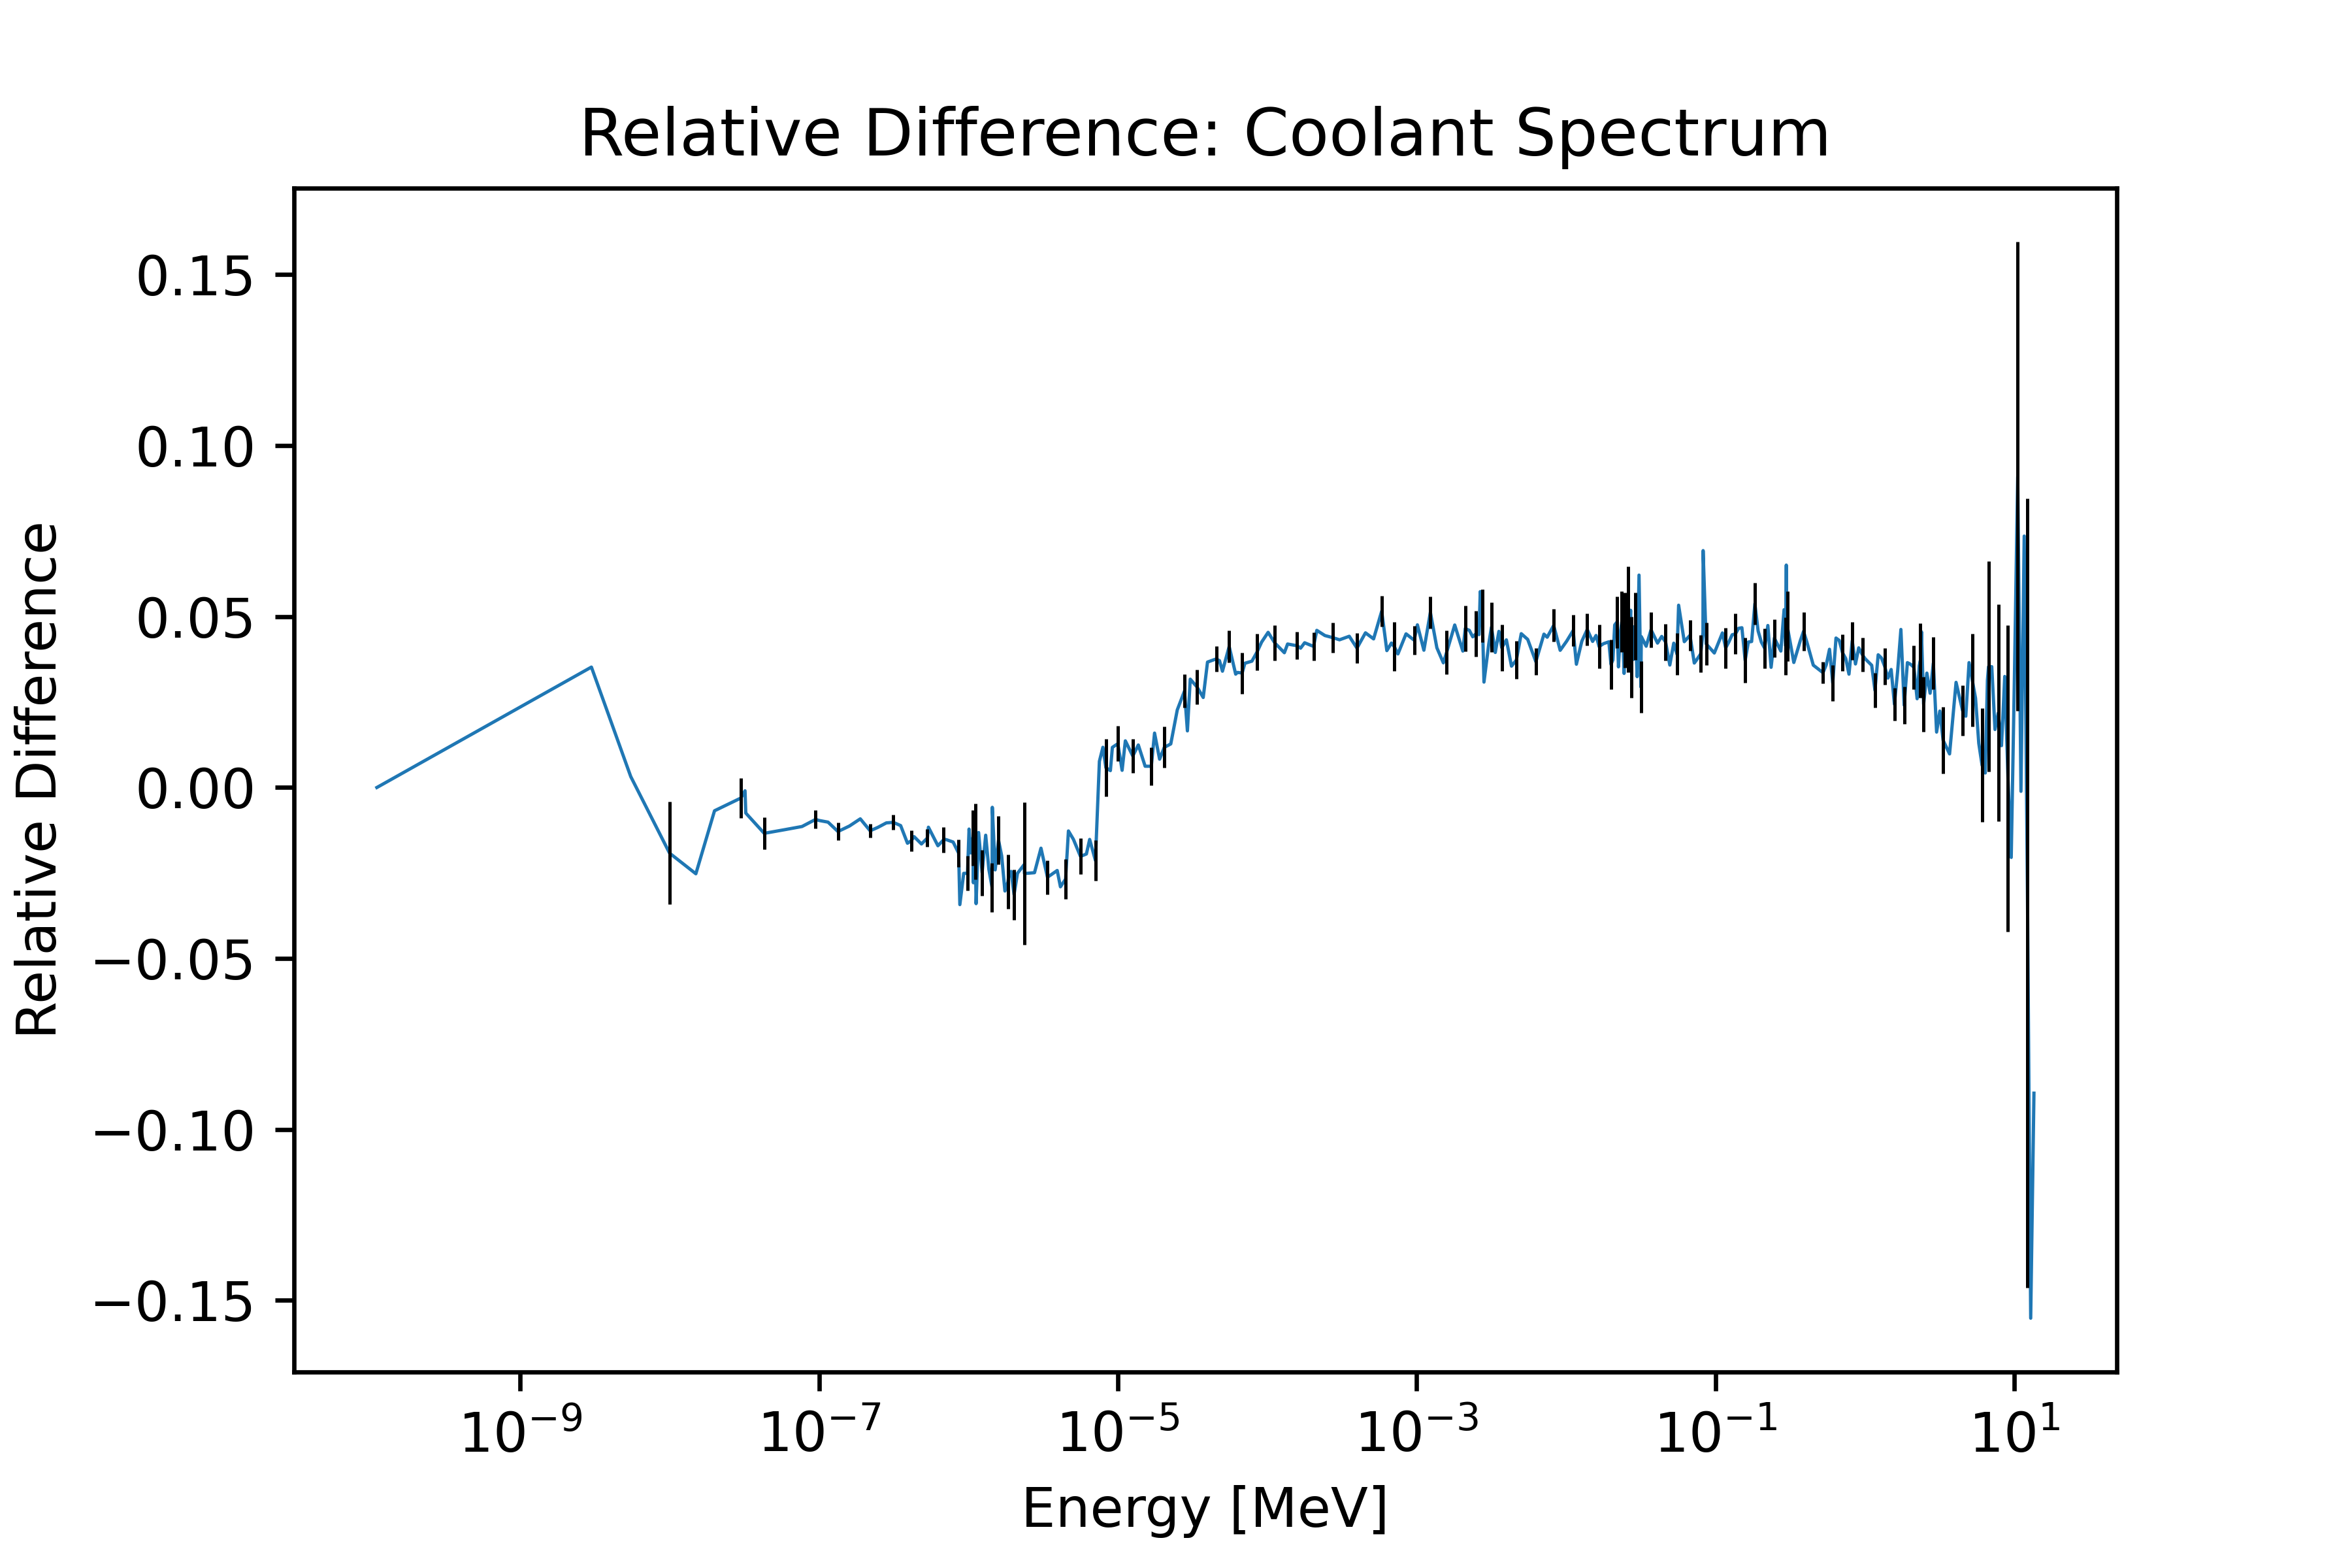
\includegraphics[width=0.95\linewidth]{figures/reldiff_cool_spec_er}
  \caption{Coolant}
  \label{fig:diff-cool}
\end{subfigure}%

\caption[]{(cont.)}
\end{figure}

\begin{figure}[H]\ContinuedFloat
\centering

\begin{subfigure}{0.95\textwidth}
  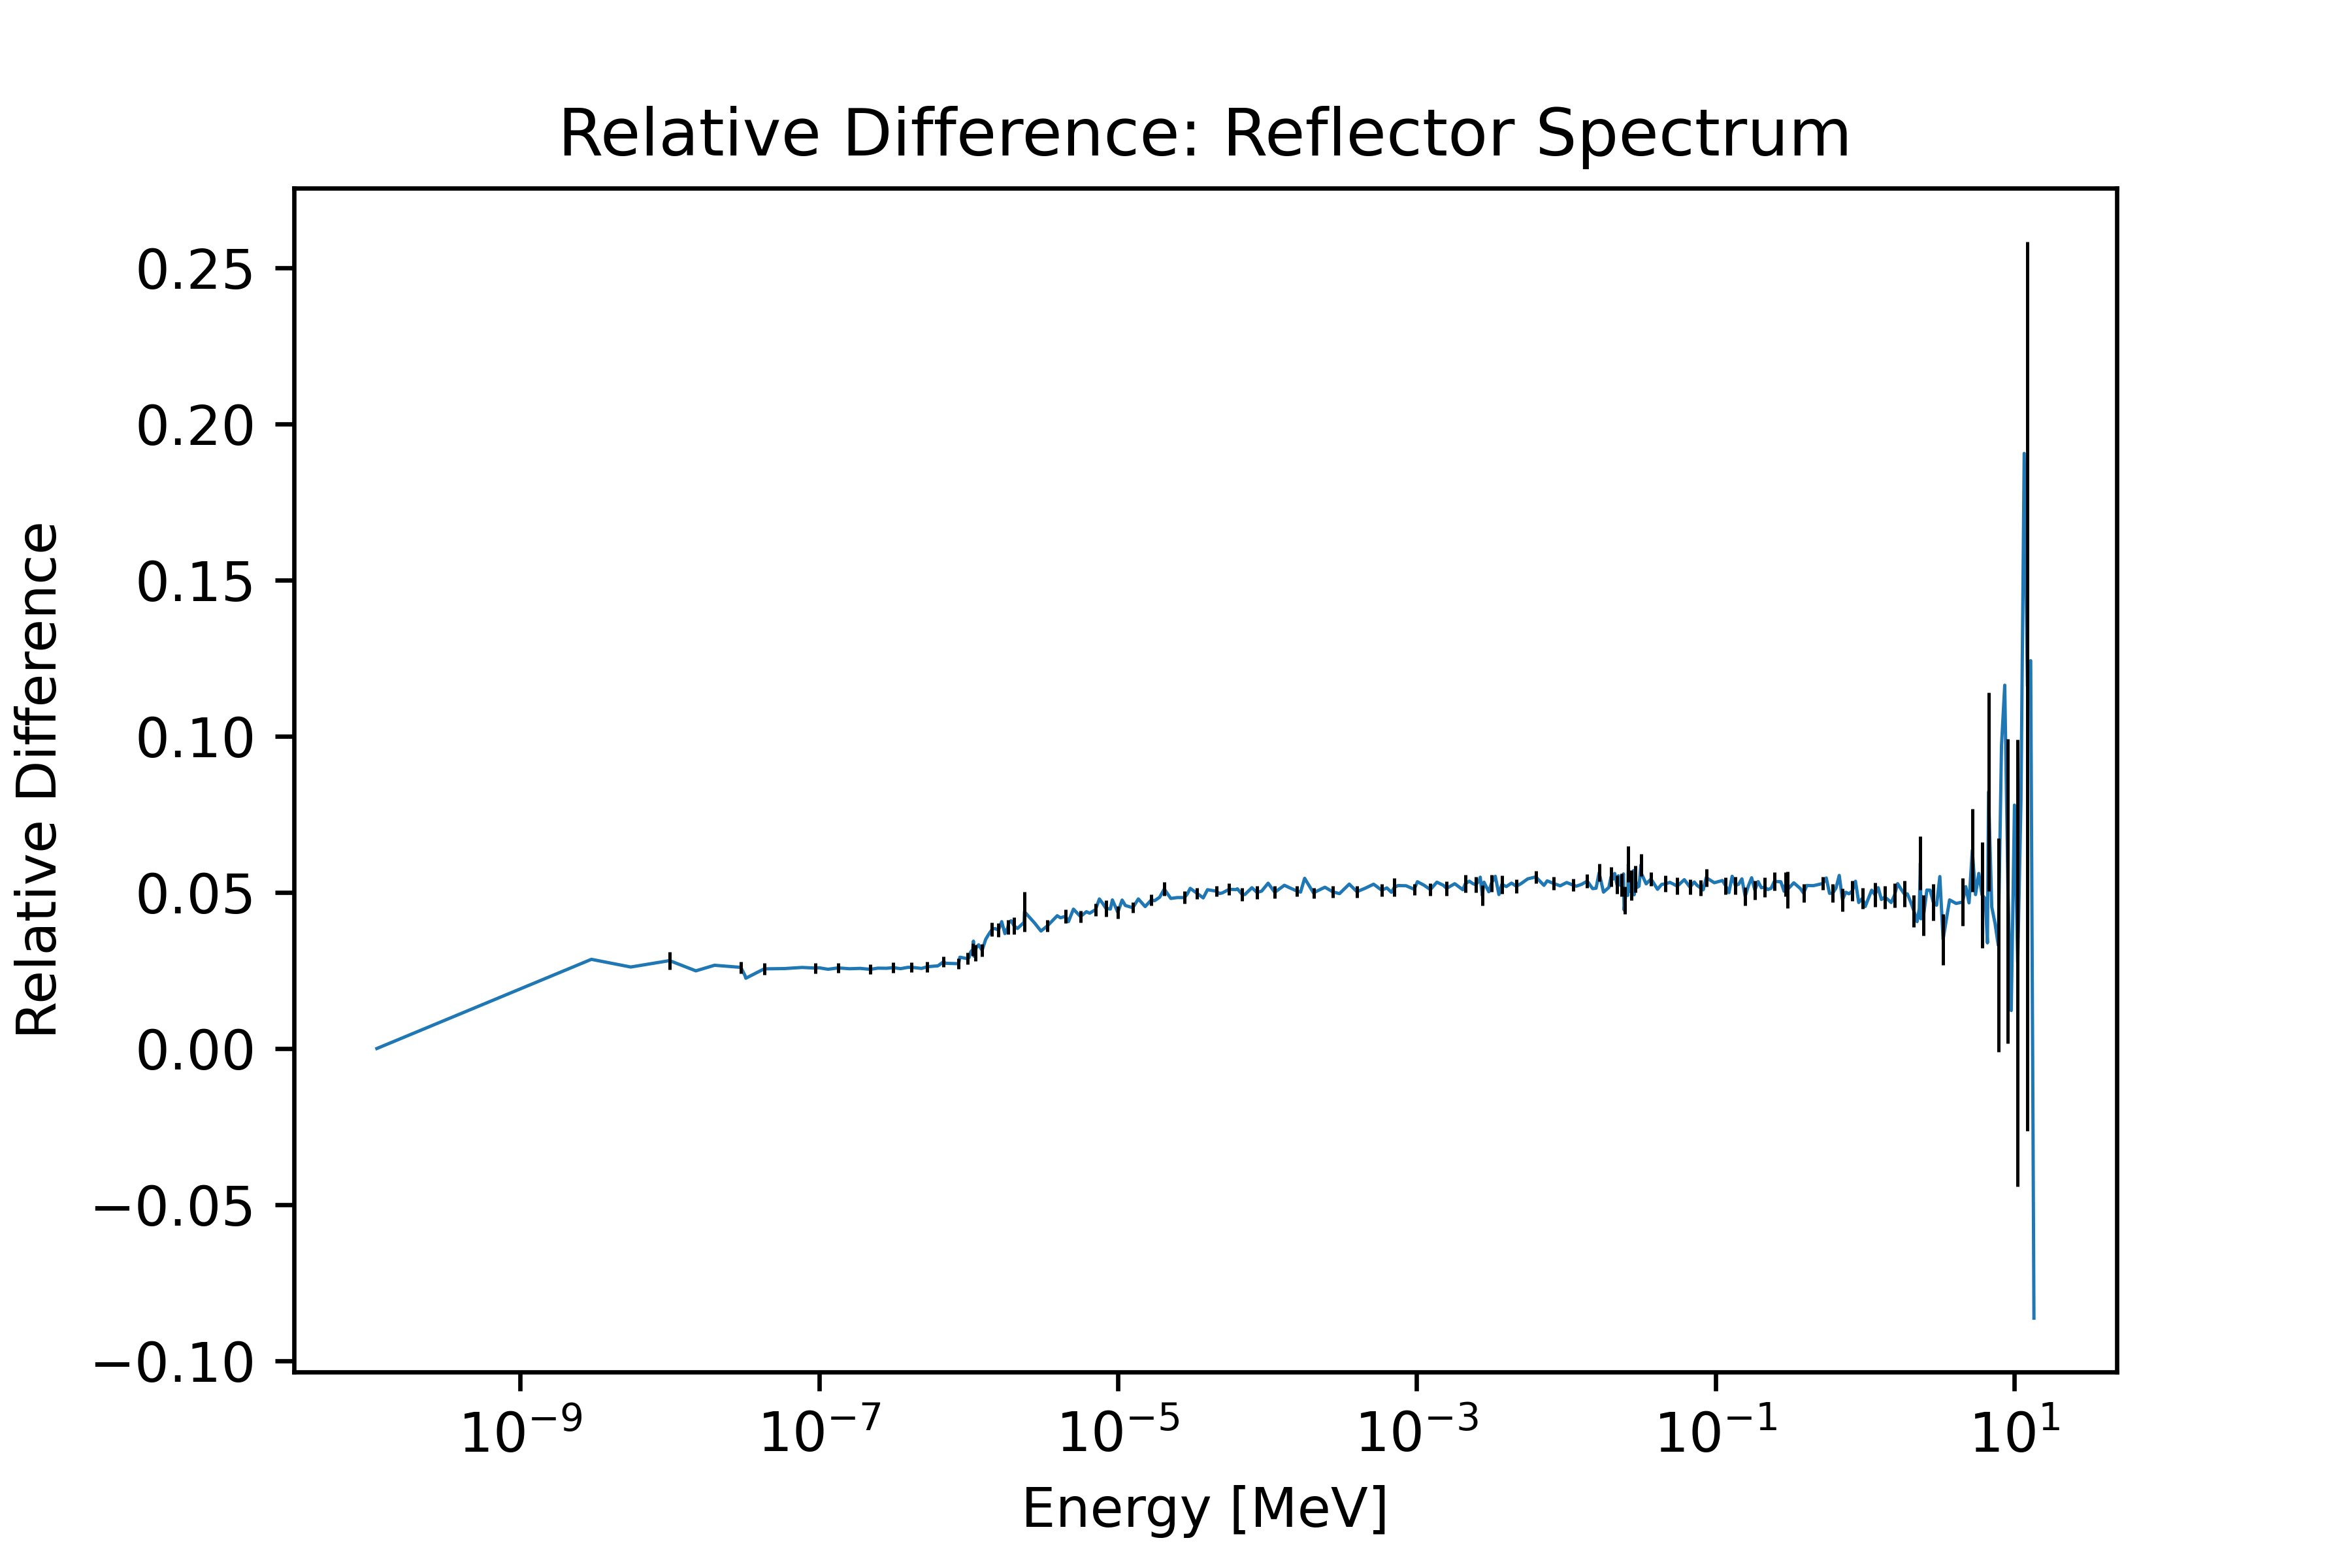
\includegraphics[width=0.95\linewidth]{figures/reldiff_reflec_spec_er}
  \caption{Reflector}
  \label{fig:diff-reflec}
\end{subfigure}%

\caption[]{(cont.)}
\label{fig:diff-spec}
\end{figure}

Overall, the homogenized model is over-predicting the thermal peak compared to the heterogenized model in the core spectra by approximately 5\%.  At approximately 10E-06 MeV, just after the thermal peak, the two spectra have a brief moment of agreement before diverging again, this time with a slightly larger disagreement.  Unlike \ref{fig:diff-flux}, the relative differences seen in in \ref{fig:diff-spec} are not accounted for by error alone, with the exception of the highest neutron energy ranges. ***should I leave these, and include an image that gives a close up of the areas of interest, so the huge error at the tail end doesn't keep the reader from seeing detail?***  

The coolant spectra differed from each other after the thermal peak in a magnitude and shape matching the differences in core spectra.  Unlike the core, however, the coolant has much closer agreement at lower energy levels, including at the thermal peak.  The reflector shows, if any, a very slight over estimation on the part of the homogeneous spectra, which is consistent for all but the highest energy levels.

It is in the pebble spectra that we see the most dramatic disagreement.  Around the thermal peak, in both \ref{fig:diff-fresh} and \ref{fig:diff-six}, there is a spike in the relative difference, though the error is still substantial in this region compared to the peaks in the relative difference.  Between the thermal peak and ~5E-02, the differences are minimal and can be accounted for by noise or error.  Between 10E-02 and 10E-01, however, there is a slight blip, which may be indicative of a fission product with a resonance around this region **I don't think I said that quite right*** being affected by having graphite surrounding it more directly.

The most dramatic peaks occur in the six-pass pebble at 0.2995 MeV, which indicates that the homogenized reactor is over-predicting the lethargy-adjusted neutron flux at this energy level.  To be precise, the homogenized pebble model is over-predicting in this region by a factor of 2.69.  In both the fresh and six-pass pebble spectra, there is a peak at *****.  One possibility is that the U-235 in the pebble is more likely to undergo fission in a homogenized pebble, which disperses the U-235 atoms in what is almost pure graphite, compared to the heterogenized pebbles, which, while some U-235 atoms may be directly next to graphite, are most like near other U-235 atoms.  That the peak in the fresh pebble is so much higher - a factor of 4 - compared to the six-pass pebble - a factor of 2 - also is another sign.



\section{Sensitivity Tests}
Beyond a comparison of homogenized versus heterogenized pebbles, the effects of two other model changes were investigated.  The first looks at the effects of assuming a $\frac{1}{6}$ core symmetry, the other is a simplified test of changing pebble locations - changing the fuel composition in each pebble, rather than entirely re-generating pebble locations using the dispersal routine.  All tests compare models using the homogenized pebble assumption as a base.

\subsection{Effects of Symmetry Assumption}

Overall, the effects of using a $\frac{1}{6}$ core symmetry were minimal.



\begin{table}[H]
\centering
\caption{Symmetry Run Results Summary}
 \begin{tabularx}{0.7\textwidth}{c  c  c  c  c}
 	\hline
 	Run & $k_{eff}$ & $k_{eff}$ $\% \Delta$ & $J^+$  $[\frac{n}{cm^2s}]$ & $J^+$ $\% \Delta$  \\
 	\hline
 	Run 1 & 1.03990 $\pm$ 0.00055 & 0.0836$\%$ & $5.921\times10^{11}$ $\pm$ $8.704\times10^{08}$ & 0.626$\%$ \\
 	Run 2 & 1.03979 $\pm$ 0.00050 & 0.0942$\%$ & $5.884\times10^{11}$ $\pm$ $8.296\times10^{08}$ & 0.010$\%$ \\
 	Run 3 & 1.04150 $\pm$ 0.00054 & 0.0701$\%$ & $5.908\times10^{11}$ $\pm$ $7.444\times10^{08}$ & 0.392$\%$ \\
 	Run 4 & 1.03927 $\pm$ 0.00057 & 0.144$\%$ & $5.910\times10^{11}$ $\pm$ $8.687\times10^{08}$ & 0.425$\%$ \\
 	Run 5 & 1.04154 $\pm$ 0.00054 & 0.0740$\%$ & $5.884\times10^{11}$ $\pm$ $8.885\times10^{08}$ & 0.010$\%$ \\
 	Run 6 & 1.04047 $\pm$ 0.00050 & 0.0288$\%$ & $5.888\times10^{11}$ $\pm$ $8.478\times10^{08}$ & 0.057$\%$ \\
 	\hline

 \end{tabularx}
\label{table:slicesens}
\end{table}

Below, \ref{fig:0-60} provides cross-sections of the geometry, and fission rate/thermal flux meshes for the one-sixth core symmetry test.  The fission rate mesh naturally exhibits a repeating pattern with six-points of symmetry, and still shows the banding patterns on the outer edges. 


\begin{figure}[h!]
\centering

\begin{subfigure}{0.45\textwidth}
  \includegraphics[width=0.95\linewidth]{figures/0-60/0-60-r}
  \caption{Radial Cross Section at y=0}
  \label{fig:0-60-r}
\end{subfigure}%
%
\begin{subfigure}{0.45\textwidth}
  \includegraphics[width=0.95\linewidth]{figures/0-60/0-60-rm}
  \caption{Radial Mesh}
  \label{fig:0-60-rm}
\end{subfigure}

\begin{subfigure}{0.45\textwidth}
  \includegraphics[width=0.95\linewidth]{figures/0-60/0-60-v}
  \caption{Axial Cross Section at z=0 }
  \label{fig:0-60-v}
\end{subfigure}
%
\begin{subfigure}{0.45\textwidth}
  \includegraphics[width=0.95\linewidth]{figures/0-60/0-60-vm}
  \caption{Axial Mesh}
  \label{fig:0-60-vm}
\end{subfigure}
%
\caption{Sensitivity Analysis: $0^{\circ}$ - $60^{\circ}$}
\label{fig:0-60}
\end{figure}
*** alright, I tried to convey my observation as best I could, but I have a suspicion it isn't nearly as clear on paper as it is in my head.  Any suggestions are welcome, and if it seems like it would be better to leave this section out, I can***
One point of interest, however, is the degree to which the region from 0 to 60 degrees matches the same region in the control model.  Figure \ref{fig:htgr-diff} was generated by subtracting the radial meshes for the control and first symmetry test.

\begin{figure}[h!]
\centering
\includegraphics[width=0.6\linewidth]{figures/htgr-diff}
\caption{An Image Generated by Subtracting \ref{fig:0-60-rm} from \ref{fig:htgr-diff}.}
\label{fig:htgr-diff}
\end{figure}

Unsurprisingly, in the areas outside the 0 to 60 degree slice, the two fission rate meshes disagree quite a bit.  However, within this region, the two meshes are almost identical, pixel for pixel.  While this might be expected towards the center of this region, the perfect match towards the edges of it are less so.  As a reminder, the symmetry tests all use a one-sixth symmetry, and a periodic boundary condition, i.e., when a neutron leaves the slice on one side, it re-enters the slice on the other.  In effect, the edges of the 0-60 slice in the symmetry test are seeing entirely different materials, compared to the control.  That there is not a gradient of difference at the edges in \ref{fig:htgr-diff}, but rather a hard line, may suggest that, with proper mixing, nearest-neighbor pebbles do not have a very strong effect.  However, it is important to note that Sangamon20 uses only fuel pebbles, and this observation may not hold true in a reactor design using, for example, adsorber pebbles. 

***I think I should put these in the appendix and directly reference them here - there just isn't enough "new" to say for each of the figures that warrants them all being in the main body, I think?***
\begin{figure}[h!]
\centering

\begin{subfigure}{0.45\textwidth}
  \includegraphics[width=0.95\linewidth]{figures/60-120/60-120-r}
  \caption{Radial Cross Section at y=0}
  \label{fig:bstep0}
\end{subfigure}%
%
\begin{subfigure}{0.45\textwidth}
  \includegraphics[width=0.95\linewidth]{figures/60-120/60-120-rm}
  \caption{Radial Mesh}
  \label{fig:bstep1}
\end{subfigure}

\begin{subfigure}{0.45\textwidth}
  \includegraphics[width=0.95\linewidth]{figures/60-120/60-120-v}
  \caption{Axial Cross Section at z=0 }
  \label{fig:bstep1}
\end{subfigure}
%
\begin{subfigure}{0.45\textwidth}
  \includegraphics[width=0.95\linewidth]{figures/60-120/60-120-vm}
  \caption{Axial Mesh}
  \label{fig:bstep1}
\end{subfigure}
%
\caption{Sensitivity Analysis: $60^{\circ}$ - $120^{\circ}$}
\label{fig:60-120}
\end{figure} 


\begin{figure}[H]
\centering

\begin{subfigure}{0.45\textwidth}
  \includegraphics[width=0.95\linewidth]{figures/120-180/120-180-r}
  \caption{Radial Cross Section at y=0}
  \label{fig:120-180-r}
\end{subfigure}%
%
\begin{subfigure}{0.45\textwidth}
  \includegraphics[width=0.95\linewidth]{figures/120-180/120-180-rm}
  \caption{Radial Mesh}
  \label{fig:120-180-rm}
\end{subfigure}

\begin{subfigure}{0.45\textwidth}
  \includegraphics[width=0.95\linewidth]{figures/120-180/120-180-v}
  \caption{Axial Cross Section at z=0 }
  \label{fig:120-180-v}
\end{subfigure}
%
\begin{subfigure}{0.45\textwidth}
  \includegraphics[width=0.95\linewidth]{figures/120-180/120-180-vm}
  \caption{Axial Mesh}
  \label{fig:120-180-vm}
\end{subfigure}
%
\caption{Sensitivity Analysis: $120^{\circ}$ - $180^{\circ}$}
\label{fig:120-180}
\end{figure}
\begin{itemize}
\item as above, but the 120-180 degree slice
\end{itemize}

\begin{figure}
\centering

\begin{subfigure}{0.45\textwidth}
  \includegraphics[width=0.95\linewidth]{figures/180-240/180-240-r}
  \caption{Radial Cross Section at y=0}
  \label{fig:bstep0}
\end{subfigure}%
%
\begin{subfigure}{0.45\textwidth}
  \includegraphics[width=0.95\linewidth]{figures/180-240/180-240-rm}
  \caption{Radial Mesh}
  \label{fig:bstep1}
\end{subfigure}

\begin{subfigure}{0.45\textwidth}
  \includegraphics[width=0.95\linewidth]{figures/180-240/180-240-v}
  \caption{Axial Cross Section at z=0 }
  \label{fig:bstep1}
\end{subfigure}
%
\begin{subfigure}{0.45\textwidth}
  \includegraphics[width=0.95\linewidth]{figures/180-240/180-240-vm}
  \caption{Axial Mesh}
  \label{fig:bstep1}
\end{subfigure}
%
\caption{Sensitivity Analysis: $180^{\circ}$ - $240^{\circ}$}
\label{fig:180-240}
\end{figure}
\begin{itemize}
\item as above, but the 180-140 degree slice
\end{itemize}

\begin{figure}
\centering

\begin{subfigure}{0.45\textwidth}
  \includegraphics[width=0.95\linewidth]{figures/240-300/240-300-r}
  \caption{Radial Cross Section at y=0}
  \label{fig:bstep0}
\end{subfigure}%
%
\begin{subfigure}{0.45\textwidth}
  \includegraphics[width=0.95\linewidth]{figures/240-300/240-300-rm}
  \caption{Radial Mesh}
  \label{fig:bstep1}
\end{subfigure}

\begin{subfigure}{0.45\textwidth}
  \includegraphics[width=0.95\linewidth]{figures/240-300/240-300-v}
  \caption{Axial Cross Section at z=0 }
  \label{fig:bstep1}
\end{subfigure}
%
\begin{subfigure}{0.45\textwidth}
  \includegraphics[width=0.95\linewidth]{figures/240-300/240-300-vm}
  \caption{Axial Mesh}
  \label{fig:bstep1}
\end{subfigure}
%
\caption{Sensitivity Analysis: $240^{\circ}$ - $300^{\circ}$}
\label{fig:240-300}
\end{figure}
\begin{itemize}
\item as above, but the 240-300 degree slice
\end{itemize}

\begin{figure}[H]
\centering

\begin{subfigure}{0.45\textwidth}
  \includegraphics[width=0.95\linewidth]{figures/300-360/300-360-r}
  \caption{Radial Cross Section at y=0}
  \label{fig:bstep0}
\end{subfigure}%
%
\begin{subfigure}{0.45\textwidth}
  \includegraphics[width=0.95\linewidth]{figures/300-360/300-360-rm}
  \caption{Radial Mesh}
  \label{fig:bstep1}
\end{subfigure}

\begin{subfigure}{0.45\textwidth}
  \includegraphics[width=0.95\linewidth]{figures/300-360/300-360-v}
  \caption{Axial Cross Section at z=0 }
  \label{fig:bstep1}
\end{subfigure}
%
\begin{subfigure}{0.45\textwidth}
  \includegraphics[width=0.95\linewidth]{figures/300-360/300-360-vm}
  \caption{Axial Mesh}
  \label{fig:bstep1}
\end{subfigure}
%
\caption{Sensitivity Analysis: $300^{\circ}$ - $360^{\circ}$}
\label{fig:300-360}
\end{figure}
\begin{itemize}
\item as above, but the 300-360 degree slice
\end{itemize}

\subsection{Effects of Pebble Shuffling}

The final test on the effects of changes to core modeling is another test of consistency between similar HTGR models with a different pebble configurations.  Rather than re-generate the pebble locations several times, the 'shuffling' test simply reassigns each pebble with a different fuel composition.  For example, the pebbles that were once fresh are now first-pass, the first pass pebbles are now second-pass, and so on.  This shuffling was done several times, and the results of this test are in \ref{table:shufsens}.



\begin{table}[H]
\centering
 \begin{tabularx}{0.7\textwidth}{c  c  c  c  c}
 	\hline
 	Run & $k_{eff}$ & $k_{eff}$ $\% \Delta$ & $J^+$  $[\frac{n}{cm^2s}]$ & $J^+$ $\% \Delta$ \\
 	\hline
 	Run 1 & 1.03994 $\pm$ 0.00054 & 0.0797$\%$ & $5.897\times10^{11}$ $\pm$ $8.668\times10^{08}$ & 0.211$\%$ \\
 	Run 2 & 1.03999 $\pm$ 0.00055 & 0.0749$\%$ & $5.902\times10^{11}$ $\pm$ $8.086\times10^{08}$  & 0.295$\%$ \\
 	Run 3 & 1.04002 $\pm$ 0.00053 & 0.0721$\%$ & $5.896\times10^{11}$ $\pm$ $8.490\times10^{08}$ & 0.192$\%$  \\
 	Run 4 & 1.04103 $\pm$ 0.00057 & 0.0249$\%$ & $5.884\times10^{11}$ $\pm$ $9.355\times10^{08}$ & 0.013$\%$ \\
 	Run 5 & 1.03960 $\pm$ 0.00053 & 0.112$\%$ & $5.904\times10^{11}$ $\pm$ $8.443\times10^{08}$ & 0.329$\%$  \\
 	Run 6 & 1.04014 $\pm$ 0.00057 & 0.0605$\%$ & $5.898\times10^{11}$ $\pm$ $7.726\times10^{08}$ & 0.227$\%$ \\
 	\hline

 \end{tabularx}
\caption{Shuffling Run Summary}
\label{table:shufsens}
\end{table}

Overall, much like the symmetry test, re-mixing the pebbles had little effect on overall results.  Likely, provided the pebbles are sufficiently mixed, and there are not 'pockets' of like pebbles, models that are otherwise identical should provide similar results. 